\documentclass[conference,compsoc]{IEEEtran}

% \usepackage{usenix-2020-09}

% \hypersetup{                    
%   colorlinks,
%   linkcolor={green!60!black},   % darker green than usenix default
%   citecolor={red!70!black},
%   urlcolor={blue!70!black}
% }

\ifCLASSOPTIONcompsoc
  % IEEE Computer Society needs nocompress option
  % requires cite.sty v4.0 or later (November 2003)
  \usepackage[nocompress]{cite}
\else
  % normal IEEE
  \usepackage{cite}
\fi

\ifCLASSINFOpdf
  % \usepackage[pdftex]{graphicx}
  % declare the path(s) where your graphic files are
  % \graphicspath{{../pdf/}{../jpeg/}}
  % and their extensions so you won't have to specify these with
  % every instance of \includegraphics
  % \DeclareGraphicsExtensions{.pdf,.jpeg,.png}
\else
  % or other class option (dvipsone, dvipdf, if not using dvips). graphicx
  % will default to the driver specified in the system graphics.cfg if no
  % driver is specified.
  % \usepackage[dvips]{graphicx}
  % declare the path(s) where your graphic files are
  % \graphicspath{{../eps/}}
  % and their extensions so you won't have to specify these with
  % every instance of \includegraphics
  % \DeclareGraphicsExtensions{.eps}
\fi

% to be able to draw some self-contained figs
\usepackage{tikz}
\usepackage{amsmath}
\usepackage{booktabs}
\usepackage{caption}
\usepackage{graphicx}
\usepackage{subfigure} % or subfigure
% inlined bib file
\usepackage{makecell}
\usepackage{filecontents}
\usepackage{adjustbox}
\usepackage{multirow}
\usepackage{xspace}
\usepackage{siunitx}
\usepackage{listings}
%% need:  sudo apt -y install texlive-science 
\usepackage{hyperref}
\usepackage{listings}
\usepackage{xcolor}
\usepackage{courier} % Use Courier for a more compact font

\definecolor{keywordcolor}{rgb}{0.5,0,0.5}
\definecolor{stringcolor}{rgb}{0.2,0.6,0.2}
\definecolor{commentcolor}{rgb}{0.5,0.5,0.5}
\definecolor{backgroundcolor}{rgb}{0.95,0.95,0.92}

% \lstset{
%     backgroundcolor=\color{backgroundcolor},
%     basicstyle=\ttfamily\footnotesize,
%     keywordstyle=\color{keywordcolor}\bfseries,
%     stringstyle=\color{stringcolor},
%     commentstyle=\color{commentcolor}\itshape,
%     numbers=left,
%     numberstyle=\tiny\color{gray},
%     stepnumber=1,
%     numbersep=10pt,
%     tabsize=4,
%     showspaces=false,
%     showstringspaces=false,
%     breaklines=true,
%     frame=single,
%     language=Java
% }


\usepackage{color}
\definecolor{lightgray}{rgb}{.9,.9,.9}
\definecolor{darkgray}{rgb}{.4,.4,.4}
\definecolor{purple}{rgb}{0.65, 0.12, 0.82}

\lstdefinelanguage{JavaScript}{
  keywords={typeof, new, true, false, catch, function, return, 
            null, catch, switch, var, if, in, while, 
            do, else, case, break,
            contract, uint256, require, address, external, 
            memory, uint, for, emit, virtual, private, event,
            uint64},
  keywordstyle=\color{keywordcolor}\bfseries,
  ndkeywords={class, export, boolean, throw, implements, import, this},
  ndkeywordstyle=\color{darkgray}\bfseries,
  identifierstyle=\color{black},
  sensitive=false,
  comment=[l]{//},
  morecomment=[s]{/*}{*/},
  commentstyle=\color{commentcolor}\ttfamily,
  stringstyle=\color{stringcolor}\ttfamily,
  morestring=[b]',
  morestring=[b]"
}

\lstset{
    % backgroundcolor=\color{backgroundcolor},
    basicstyle=\ttfamily\footnotesize,
    keywordstyle=\color{keywordcolor}\bfseries,
    stringstyle=\color{stringcolor},
    commentstyle=\color{commentcolor}\itshape,
    % numbers=left,
    % numberstyle=\tiny\color{gray},
    stepnumber=1,
    numbersep=10pt,
    tabsize=4,
    showspaces=false,
    showstringspaces=false,
    breaklines=true,
    frame=none,
    % frame=single,
    % xleftmargin=8pt,
    % numbersep=8pt,
    % framexleftmargin=8pt,
    language=JavaScript
}

% \lstset{
%    language=JavaScript,
%    backgroundcolor=\color{lightgray},
%    extendedchars=true,
%    basicstyle=\footnotesize\ttfamily,
%    showstringspaces=false,
%    showspaces=false,
%    numbers=left,
%    numberstyle=\footnotesize,
%    numbersep=9pt,
%    tabsize=2,
%    breaklines=true,
%    showtabs=false,
%    captionpos=b
% }


\newenvironment{CompactItemize}%
  {\begin{list}{$\triangleright$}%
    {\leftmargin=\parindent \itemsep=2pt \topsep=2pt
     \parsep=0pt \partopsep=0pt}}%
  {\end{list}}
\renewcommand{\labelitemi}{$\triangleright$}



\newcommand{\offlinetool}{CrossChecked\xspace} % xspace is double-edged...
\newcommand{\onlinetool}{Big Bro\xspace}
\newcommand{\newarch}{your definition here~}


\newcommand{\bil}{\textsc{b}\xspace}
\newcommand{\mil}{\textsc{m}\xspace}
\newcommand{\thou}{\textsc{k}\xspace}

\begin{document}
\title{Count of Monte Crypto: Accounting-based Defenses for Cross-Chain Bridges} % TODO: replace with your title



% \author{
% {\rm Enze Liu, Elisa Luo, Jian Chen Yan, Katherine Izhikevich, Stewart Grant,\\ Deian Stefan, Geoffrey M Voelker, Stefan Savage}\\
% UC San Diego
% }


\iffalse
\newcommand{\alex}[1]{\textcolor{red}{\noindent[AL: #1]}}
\newcommand{\elisa}[1]{\textcolor{blue}{\noindent[EL: #1]}}
\newcommand{\geoff}[1]{\textcolor{teal}{[GV: #1]}}
\newcommand{\deian}[1]{\textcolor{green}{[ds: #1]}}
\else
\newcommand{\alex}[1]{}
\newcommand{\elisa}[1]{}
\newcommand{\geoff}[1]{}
\newcommand{\deian}[1]{}
\fi

\maketitle

\begin{abstract}
Between 2021 and 2023, crypto assets valued at over \$US2.6 billion
were stolen via attacks on ``bridges'' --- decentralized services
designed to allow inter-blockchain exchange.  While the individual
exploits in each attack vary, a single design flaw underlies them all:
the lack of end-to-end value accounting in cross-chain transactions.
In this paper, we empirically analyze over 10\mil million transactions used
by key bridges during this period.  We show that a simple invariant
that balances cross-chain inflows and outflows is compatible with
legitimate use, yet precisely identifies every known attack (and
several likely attacks) in this data.  Further, we show that this
approach is not only sufficient for post-hoc audits, but can be
implemented in-line in existing bridge designs to provide generic
protection against a broad array of bridge vulnerabilities.
\end{abstract}


\begin{dissertationintroduction}
% Start by giving a brief description of 
% what the hack is service composition. 
Service composition is a common practice in modern software systems, where multiple independently developed services interact with each other using predefined protocols. This practice is common in modern software development and offers many benefits. For example, it allows individual services to be developed and maintained independently, which can lead to faster development cycles and easier updates. Further, individual services can be reused within an application or 
across different applications, promoting modularity and reducing redundancy in code.

While beneficial, the security community has also recognized that this practice creates a new set of security concerns. Namely, services can make inconsistent assumptions about how they interact with each other. Indeed, prior work such as has highlighted that these assumptions exist at low levels. For example, one service may assume that another service will provide input data in a specific format, while the second service may not 
be aware of or enforce this assumption. As a result, an attacker can exploit these inconsistencies and craft adversarial inputs that bypass certain security controls.
Chen et al.~\cite{chen2020composition} highlighted the security risks associated with these inconsistencies
using email as a case study. Similarly, other work (e.g., ~\cite{other2020study}) has also explored these issues in different contexts.\todo{todo find some citations}

% Now, transition into the point that prior work ignored high-level assumptions because they are less well-specified.

However, prior work has primarily focused on assumptions made at low levels, such as input data formats. This concentration is likely because these low-level assumptions are more concrete and easier to analyze, as they are expressed in code. Indeed, the community has developed a variety of techniques, such as fuzzing, static analysis and machine learning, to reason about these low-level assumptions. 

% Now, meniton high-level assumptions also exist. because they are less well-specified.
What has been largely ignored, however, are high-level assumptions, such as how services will be used. These aspects are less well-specified and often abstract. 
To make matters worse, reasoning about the security implications of these assumptions is more challenging because they often require a holistic understanding of the system. As a result, traditional security techniques that focus on low-level code and individual components are often ineffective for studying these high-level assumptions.

As a concrete example, consider the case of email forwarding. When a user sets up email forwarding, they typically assume that the forwarding service will handle the email in a specific way, such as preserving the original sender's information. However, if the forwarding service does not enforce this assumption, an attacker could exploit this inconsistency to send emails that appear to come from a trusted source, thereby bypassing email security measures.

My work aims to address this gap by systematically identifying and analyzing high-level assumptions in service composition and their security implications. I propose a holistic, end-to-end approach. Using this approach, I systematically identify the assumptions made by services in three systems: email, Android, and cross-chain bridges.

In the first case study, I analyze the assumptions made by email services and demonstrate how these assumptions do not always hold in practice, leading to security vulnerabilities. I show how these vulnerabilities can be exploited to bypass email authentication mechanisms, allowing attackers to impersonate legitimate senders and forge emails.

In the second case study, I focus on the Android operating system and its API services. I identify assumptions made by Android apps regarding the behavior of the underlying system and demonstrate how these assumptions can lead to vulnerabilities that allow malicious apps to perform persistent surveillance on target devices.

In the third case study, I examine cross-chain bridges in the context of blockchain technology. I identify assumptions made by these bridges regarding the behavior of different blockchains and demonstrate how these assumptions can lead to vulnerabilities that allow attackers to exploit inconsistencies between chains, resulting in significant financial losses.



% I propose an end-to-end methodology for identifying and mitigating security risks in service composition. This methodology combines formal verification techniques with empirical testing to provide a comprehensive understanding of the security landscape in service-oriented architectures.


% 


% Instead, a more holistic perspective is needed to understand and mitigate the security risks associated with service composition.



% for reasoning about security vulnerabilities often focus on low-level code, such as buffer overflows or memory corruption, but these techniques are not well-suited for reasoning about the higher-level abstractions and protocols that govern service interactions.


% Component-based software design is a primary engineering
% approach for building modern software systems. This pro-
% gramming paradigm, however, creates security concerns due
% to the potential for inconsistent interpretations of messages be-
% tween different components. In this paper, we leverage such
% inconsistencies to identify vulnerabilities in email systems.
% We identify a range of techniques to induce inconsistencies
% among different components across email servers and clients.
% We show that these inconsistencies can enable attackers to
% bypass email authentication to impersonate arbitrary senders,
% and forge DKIM-signed emails with a legitimate site’s signa-
% ture. Using a combination of manual analysis and black-box
% testing, we discovered 18 types of evasion exploits and tested
% them against 10 popular email providers and 19 email clients—
% all of which proved vulnerable to various attacks. Absent
% knowledge of our attacks, for many of them even a consci-
% entious security professional using a state-of-the-art email
% provider service like Gmail cannot with confidence readily
% determine, when receiving an email, whether it is forged.

% Component-based software design [1] has been widely
% adopted as a way to manage complexity and improve reusabil-
% ity. The approach divides complex systems into smaller mod-
% ules that can be independently created and reused in different
% systems. One then combines these components together to
% achieve desired functionality. Modern software systems are
% commonly built using components made by different devel-
% opers who work independently.
% While having wide-ranging benefits, the security research
% community has recognized that this practice also introduces
% security concerns. In particular, when faced with crafted ad-
% versarial inputs, different components can have inconsistent
% interpretations when operating on the input in sequence. At-
% tackers can exploit such inconsistencies to bypass security
% policies and subvert the system’s operation

% Systems today are complex than ever. This complexity not only makes it challenging to protect existing systems against known vulnerabilities, but also introduces unintended security vulnerabilities that do not fall within the purview of current threat models. In this thesis, I highlight how unintended security vulnerabilities can arise from both the complexity within a system and the complexity introduced by the interaction between already complex systems. Using Android API system as an example, I demonstrate how the complexity within this one system produces vulnerabilities that ultimately enable malicious apps to perform persistent and stealthy surveillance on a target device. I then show, through the case study of email forwarding, how the composition of email systems leads to vulnerabilities that allow an adversary to reliably evade email security protections. I conclude by discussing my ongoing work on cryptocurrency scams and hacks, which further illustrates how the complexity of various systems can enable both large-scale and targeted attacks that result in significant financial losses.

% Nowadays, software systems are extremely complicated that are not just a simple program running on a machine. Oftentimes, it involves dozens of different pieces of software that all are talking to each other. Each piece of software will make different assumptions about how users and other pieces of software are going to use the things they expose. In practice this creates problems because an adversary does not have to play by rules and follow the assumption. I study assumptions that made these individuals pieces of software and their security implications.

% My research interests are in empirically understanding and securing real-world systems, with
% a particular emphasis on complex, large-scale systems whose vulnerabilities impact a broad range of users.
% At the core of this work is identifying the range of unvalidated assumptions systems make and how those
% assumptions may be exposed to, and thus exploitable by, attackers. While fragility in low-level code is
% well-trodden ground (e.g., how invalid assumptions about array bounds can produce control flow integrity
% vulnerabilities), my work focuses on how ambiguities and assumptions in higher-level services and service
% protocols create their own unique set of challenges – particularly in the presence of composition. As I
% show, these issues emerge in diverse contexts ranging from operating system APIs, to standard e-mail
% delivery protocols, to the systems used to manage inter-blockchain financial transactions.
% A simple example of such an issue is cloud-based e-mail filtering (e.g., as provided by third-party
% companies such as Proofpoint or Barracuda). To deploy such a capability, one must compose an existing
% email delivery service (i.e., provided by the Simple Message Transport Protocol) with a separate mail
% filtering service. Thus, inbound mail must be first diverted to the filtering service which then, after
% filtering must forward the e-mail to the destination email server. However, implicit in this arrangement
% is that this composition is somehow enforced. If not, a malicious sender might bypass this filtering service
% by simply sending messages directly to the destination server.
% Thus far, it remains a challenging task to reason about service-level assumptions like this. For one,
% studying these assumptions requires reasoning about aspects that are less well-specified (e.g., the sender
% of an email follows the intended flow). Further complicating the issue is the composition of services
% — when services are combined to create new functionality, it exposes the fragility of their underlying
% assumptions, as interactions with other services can occur in unexpected ways.
% My goal is to make systems more secure, transparent, and usable at the service level, especially those
% that are user-facing and widely-deployed. Achieving this goal requires understanding how these systems
% work in practice, which in turn requires data. To this end, I have developed a variety of tools to collect
% data, such as through large-scale measurements, reverse-engineering, and user studies. I then analyze
% the collected data, understand the system and various assumptions made, identify gaps between the
% assumptions and reality (how systems are intended to work versus how they actually work), and reason
% about the security implications of these gaps. 

\end{dissertationintroduction} % TODO: replace with your brilliant paper!

% % Bridge Actually Received <= Bridge Logged Received
% Bridge Logged Withdraw >= Bridge Actually Withdraw
\begin{figure*}[h]
\centering
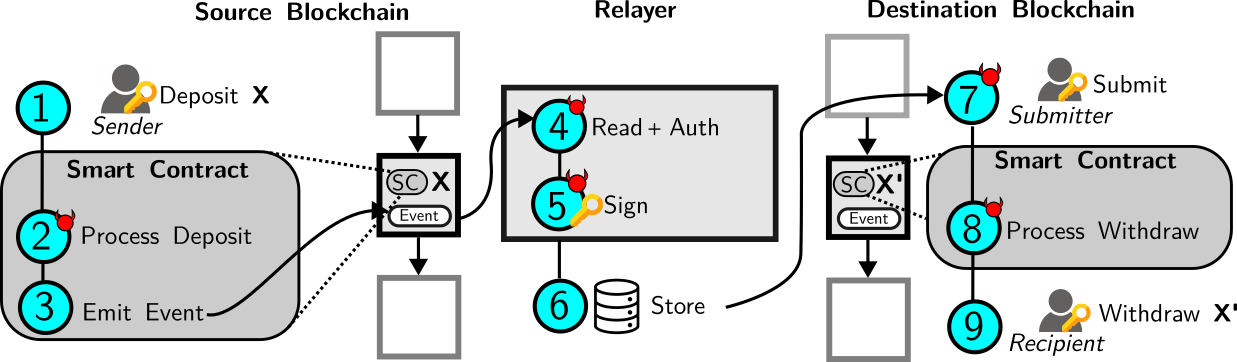
\includegraphics[width=0.8\textwidth]{fig/bridge_arch.pdf}
%%command for cropping pdf
%%gs -sDevice=pdfwrite -o bridge_arch_crop.pdf bridge_arch.pdf
\caption{Cross-chain token bridging and the different steps attackers can exploit to withdraw unbacked deposits.}
\label{fig:cross-chain}
\end{figure*}

\section{Background}
\label{sec:background}
% In this section, we start by providing an overview of blockchain technology. We then describe how cross-chain bridges work followed by the threat model we consider in this paper.
% In this section
We first give a brief introduction to smart contract blockchains
and cross-chain bridges. We then describe how bridges, under attack, collapse in
practice.

\subsection{Smart-contract Blockchains} Modern DeFi protocols (e.g.,
decentralized exchanges and lending protocols) are built on top
of ``smart-contract'' blockchains, like Ethereum. At their core, these chains, like
the original Bitcoin blockchain, are distributed ledgers that manage accounts
(public keys) and their balances (in native tokens like Ethereum's ETH). Users
interact with these chains by signing and broadcasting (to the distributed nodes
that make up the chain network) transactions that, for example, transfer
funds from their account (using the corresponding account private key) to
another user's account.

Ethereum, and the smart-contract chains it inspired since its release in 2015,
differ from Bitcoin by extending the ``simple'' distributed ledger with a smart
contract execution layer. A smart contract on Ethereum is an \emph{internal}
account---and, like a normal, \emph{externally owned} account (EOA), it has a
balance---that has associated \emph{code} (EVM bytecode), which implements the
smart contract's program logic, and \emph{storage}, which persists the program's
state across executions. Users interact with (i.e., execute) smart contracts
much like they do when transferring funds from their account: they sign a
transaction that encodes the smart contract to call (i.e., the contract address),
the particular function to execute, and the arguments to call the function with.
Instead of simply transferring funds from the user's account, then, executing
such a \emph{smart-contract call} transaction amounts to executing the smart
contract bytecode---and any smart contracts the contract itself calls.
    
% \begin{lstlisting}
% contract USDC{
%   mapping(account => amount) _balances;
%   event Transfer(from, to, value);
%   function transfer(to, amount) {
%     address from = msg.sender; // user
%     // ... validate user has enough balance
%     _balances[from] -= amount;
%     _balances[to] += amount;
%     emit Transfer(from, to, amount);
%   }

%   function mint(to, amount) {
%     _balances[to] += value;
%     emit Transfer(address(0), to, amount);
%   }

%   function burn(from, amount) {
%     // ... validate user has enough balance
%     _balances[from] -= amount;
%     emit Transfer(from, address(0), amount);
%   }

%   function safeTransferFrom(from, to, amount){ 
%     // ... transfer tokens; revert if failed
%   }
% }
% \end{lstlisting}


\begin{figure}[t]
    \centering
    \includegraphics[width=\columnwidth]{fig/usdc-contract-2sp.pdf}
    \caption{Simplified USDC ERC-20 Token Contract.}
    \label{fig:erc20}
\end{figure}


    

% \lstdefinestyle{myStyle}{
%     belowcaptionskip=1\baselineskip,
%     breaklines=true,
%     % frame=none,
%     % numbers=none, 
%     basicstyle=\footnotesize\ttfamily,
%     % keywordstyle=\bfseries\color{green!40!black},
%     % commentstyle=\itshape\color{purple!40!black},
%     % identifierstyle=\color{blue},
%     backgroundcolor=\color{gray!10!white},
%     language=Python,
% }

% \lstdefinestyle{customc}{
%   belowcaptionskip=1\baselineskip,
%   breaklines=true,
%   frame=L,
%   xleftmargin=\parindent,
%   language=Python,
%   showstringspaces=false,
%   basicstyle=\footnotesize\ttfamily,
%   keywordstyle=\bfseries\color{green!40!black},
%   commentstyle=\itshape\color{purple!40!black},
%   identifierstyle=\color{blue},
%   stringstyle=\color{orange},
% }


\subsection{ERC-20 Tokens}
One of the immediate applications of smart contracts---and to date still one of
most popular---is to create custom tokens (or coins).  To launch a new token, an
organization no longer needs to launch a new blockchain; they can instead deploy
a new contract that implements the ERC-20 token standard interface on a chain
like Ethereum and take advantage of existing on-chain infrastructure like
decentralized exchanges that make it easy to, for example, trade one kind of
token for another---both native tokens (e.g., ETH) and other tokens.\footnote{
    Most EVM chains, i.e., chains that use Ethereum's execution layer,
    follow Ethereum standards like ERC-20. Most non-EVM chains like Solana
    (which have different execution models) have similar standards (e.g., SPL
    tokens in Solana's case).
}

Figure~\ref{fig:erc20} shows a simplified variant of one such token
contract---the USDC \emph{stablecoin} contract.  This contract tracks
how many USDC tokens an account has and governs the spending of these
tokens (much like a bank governs bank notes).  For example, the
contract's \texttt{mint} function lets Circle (the company that owns
the USDC contract) mint new tokens into a user's account---e.g., after
receiving the corresponding payment from the user off-chain (in US
dollars, as USDC tokens are pegged to the US dollar).  The contract
exposes the ERC-20 interface that lets users (and smart contracts)
transfer tokens from their account by simply calling functions like
\texttt{safeTransferFrom}, and, in turn, use the tokens in any DeFi
protocol (e.g., lending the USDC to different markets, exchanging USDC
for ETH,
% buying NFTs using the USDC,
etc.). Finally, the contract's
\texttt{burn} function ``burns'' a token out of circulation---and
emits an event (Figure~\ref{fig:erc20-event}) that Circle's off-chain code looks for before allowing
a user to withdraw the corresponding USD fiat off-chain.

% \subsection{Blockchain Basics}
% In this section, we cover the basic concepts of blockchain technology, including blockchains, smart contracts, transactions, accounts, and tokens.

% \textbf{Blockchains.} A blockchain is a distributed ledger that stores data (e.g., account balance) in a transparent and tamper-proof manner. It consists of a chain of blocks, where each block contains a certain amount of data, a reference to the previous block (thus forming a chain), and other information such as timestamp. Blockchains are maintained by a network of nodes that validate data in the blocks and reach consensus on the state of the ledger.\alex{somehow have to mention Solana and Ethereum and others?}
% % It consists of a series of blocks that are linked together via cryptography (thus forming a chain) [65]. These blocks are immutable and can be used to store data (e.g., transactions). They are also maintained by a distributed network of nodes, removing the need of a central server. 

% \textbf{Smart Contracts.} Smart contracts are programs that can be executed. Typically, smart contracts are first written in high-level programming languages such as Solidity or Rust. Then, they are compiled into bytecode and deployed to the blockchain. Upon deployment, each smart contract is assigned a unique address and becomes immutable. After deployment, they can be executed based on the input provided and the logic programmed into the contract.

% % , compiled into bytecode, and deployed to the blockchain. The input and execution of smart contracts are all recorded on the blockchain. They 

% % are stored and executed on blockchains. They are used to encode business logic, enforce rules, and automate processes. Smart contracts are written in high-level programming languages, compiled into bytecode, and deployed to the blockchain. Once deployed, smart contracts are immutable and can be interacted with by sending transactions.

% % self-executing programs that run on blockchains. They are used to encode business logic, enforce rules, and automate processes. Smart contracts are written in high-level programming languages, compiled into bytecode, and deployed to the blockchain. Once deployed, smart contracts are immutable and can be interacted with by sending transactions.

% \textbf{External Owned Accounts.}  Externally owned accounts (EOAs) represent users and are controlled by private keys. Users can interact with other users or deployed smart contracts by initiating a transaction from their EOAs. To initiate a transaction, a user specifies the recipient (the address of an EOA or a smart contract), the amount of assets to transfer, and any additional input parameters required by the smart contract. 

% % are entities that can send and receive transactions on the blockchain. There are two types of accounts: externally owned accounts (EOAs) and contract accounts. EOAs are controlled by private keys and represent human users, while contract accounts are controlled by smart contracts and represent autonomous entities.

% % Accounts are entities that can send and receive transactions on the blockchain. There are two types of accounts: externally owned accounts (EOAs) and contract accounts. EOAs are controlled by private keys and represent human users, while contract accounts are controlled by smart contracts and represent autonomous entities.


% \textbf{Transactions.} A transaction is a instruction set constructed and signed by a user using their EOA. It typically includes several fields, such as the sender (the EOA that signs the transaction), the recipient (which can be an EOA or a smart contract), the amount of assets to transfer, and the input parameters required by a smart contract. Once signed, the transaction is broadcasted to the network and executed. After successful execution, the resulting state changes are recorded on the blockchain along with the transaction itself.


% \textbf{Tokens.} Every blockchain system has its own native token. For example, Ethereum has Ether (ETH), while Solana has Sol (SOL). In addition to native tokens, blockchains can also host other types of tokens. An example is ERC-20 tokens on Ethereum, which are smart contracts that follow a set of rules and standards. Of particular note, when a user transfers ERC-20 tokens, the ERC-20 token contract emits an event (a type of debug information recorded on the blockchain) that logs certain information. Figure 1 shows an example. The name of the event is Transfer, and the token contract that emits the Transfer event is tagged as USDC. The sender and recipient are represented by their addresses (0x68... and 0xF5..., respectively). The amount of tokens transferred is 212295874.

% \alex{maybe liquidity pool}


\subsection{Cross-Chain Token Bridges}
While smart contracts make it easy to launch new tokens without spinning up new
chains, there is no real shortage of new blockchains being deployed (almost weekly).  Indeed,
the modern blockchain ecosystem is a many-chain ecosystem.  Blockchains like
Avalanche, Base, and Solana have different design points---from cheaper ``gas''
execution costs, to higher throughput, lower latency, and different permission
models---that make them better suited for different classes of application.
This situation has resulted in applications that span many chains and cross-chain
infrastructure that ultimately (try to) allow users to, for example, buy
Dogwifhat NFTs on Solana using USDC tokens on Ethereum.

Core to these applications and infrastructure---and the focus of our work---is
the \emph{cross-chain token bridge}.  At a high level, a cross-chain token
bridge makes it possible for a user to ``transfer'' their tokens from one chain
(e.g., their USDC on Ethereum) to another chain (e.g., Solana) and then use the
transferred tokens on the destination chain (e.g., on a Solana exchange trading
USDC and Dogwifhat).\footnote{While some cross-chain bridges \emph{do} let users
transfer one kind of token (e.g., USDC on Ethereum) for a completely different
kind of token on the destination chain (e.g., Dogwifhat on Solana), these bridges
essentially fuse the cross-chain token bridge with an exchange (or swap). We
focus on token bridges not only because they are fundamental to other kinds of
bridges, but also because they have higher volume, more liquidity, and more
attacks.} Since smart contracts cannot make network requests or otherwise
access sate outside their own storage, a cross-chain token bridge consists of
smart contracts on both the source and destination chains, and off-chain
infrastructure that serves to relay the ``transfer'' call across the two
contracts.

\begin{figure}[t]
\centering
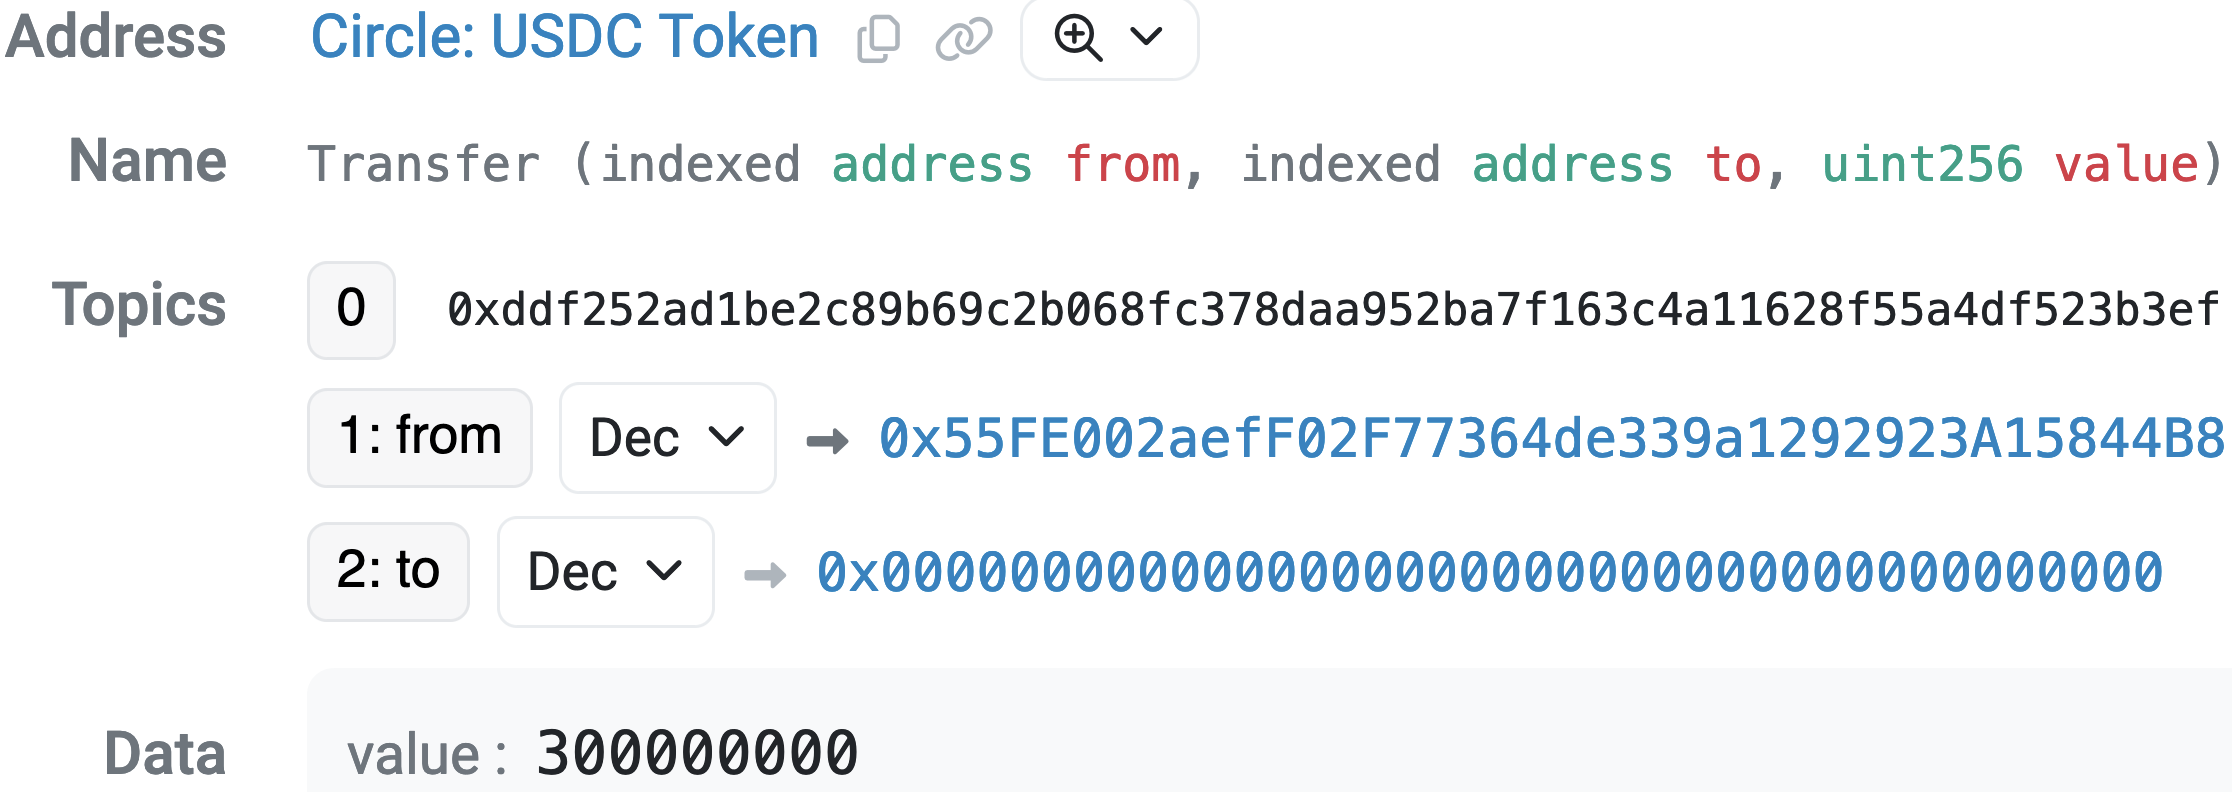
\includegraphics[width=\columnwidth]{fig/token.png}
\caption{Event Emitted by an ERC-20 Token (USDC).}
\label{fig:erc20-event}
\end{figure}

As Figure~\ref{fig:cross-chain} shows, a typical cross-chain token transfer,
i.e., a bridge transaction, consists three phases:

\textbf{1. Deposit (on source chain).}
To initiate a cross-chain token transfer, the user first calls the bridge's
contract on the source chain:
\begin{lstlisting}
deposit(address token, uint256 val, address to) {
  address from = msg.sender;  // user
  address to = address(this); // bridge contract
  // ... validate the ERC-20 token contract
  token.safeTransferFrom(from, to, val);
  emit Deposited(id++, token, from, to, val);
}
\end{lstlisting}
This contract function---a simplified version of the Qubit bridge deposit
function---processes the user's deposit (step 2) by validating the transfer request,
e.g., against a list supported tokens, and then transferring the user's ERC-20
tokens to the bridge contract---recall contracts are accounts with balances.
Then, the function emits an event (step 3) recording the user's deposit details
(including the deposit ID, the ERC-20 token contract address, the recipient on
the destination chain, and value).

\textbf{2. Off-chain relay.}
The emitted event is observed by an off-chain relayer in (step 4),
which constantly monitors the source blockchain.  The relayer first
verifies the authenticity of the deposit event.  If the event is
authentic, the relayer then produces a signed \emph{receipt}
endorsing the deposit (step 5) and, typically, stores the receipt off-chain (step
6).  Finally, this signed receipt is sent to the bridge's withdrawal contract
on the destination blockchain (step 7). Who submits the receipt varies across
bridges---some bridges submit the receipt on the user's behalf (in these cases, the
signed receipt is simply a signed contract-call transaction), while others give
users (and anyone willing to pay gas) the signed receipt and they, in turn,
submit the receipt to the withdrawal contract to complete the transfer. 

\textbf{3. Withdraw (on destination chain).}
The withdrawal contract on the destination chain first processes the withdraw
request by verifying the receipt and transferring the tokens to the recipient
(step 8). In (the simplified) Chainswap's withdraw case, for example, users call:
\begin{lstlisting}
withdraw(uint256 id, address token, address to, uint256 val, Signature[] sigs) {
  _chargeFee();
  // verify receipt
  require(received[id][to] == 0, 'withdrawn');
  for(uint i=0; i < sigs.length; i++) {
    verify_receipt(sigs[i], id, token, to, val);
  }
  received[id][to] = val; // mark as withdrawn
  token.safeTransferFrom(address(this), to, val);
  emit Withdraw(id, token, to, val);
}
\end{lstlisting}
This contract function first charges the caller a fee, then verifies the
deposit details against receipt---both that the deposit was not already
withdrawn and that the receipt signatures are valid---and finally transfers the
tokens to the intended recipient.  We consider a cross-chain transaction
complete when the asset is released to the recipient (step~9).

We expect every cross-chain bridge transaction to uphold the balance invariant:
the value (and kind) of the tokens withdrawn---the outflow---should equal the
value (and kind) of the tokens deposited---the inflow---minus the charged fees.
In practice, they do not.



% \subsection{Cross-Chain Bridges}
% In this section, we begin by providing an example of how a typical cross-chain transaction works. We then discuss the different variants of cross-chain bridges. 
% \subsubsection{A Typical Cross-Chain Transaction}
% Figure~\ref{fig:cross-chain} depicts a typical cross-chain transaction. Starting with the source blockchain, the sender (represented by their EOA) initiates a transaction to transfer assets to the bridge's deposit contract (step 1). The bridge contract then verifies that it has received the assets (step 2). Upon verification, the bridge contract emits an event to record the transfer (step 3). This event is observed by the relaying component (step 4), which typically resides outside and constantly monitors the source blockchain. The relaying component then verifies the authenticity of the event (step 5). If the event is authentic, the relaying component signs the message and stores the signature in a queryable database (step 6). A submitter on the destination blockchain then fetches the signed message from the database (step 7) and sends it to the bridge's withdrawal contract on the destination blockchain (step 8). The bridge contract then verifies the signature (step 9) and transfers the assets to the recipient (step 10). A cross-chain transaction is considered complete when the asset is released to the recipient (step 11).

% % Important things we need in this figure:
%     % source and dst amount
%     % how different vulnerabilities manifest
%         % source
%             % transfer in
%             % verify * emit
%         % relaying component
%             % observe
%             % signs
%         % dst
%             % retrieve & send
%             % verify
%             % transfer out
%     % Players
%         % Sender (in source)
%         % Relayer (in dst)
%         % Receiver (in dst)
    
    



% \subsubsection{Variants of Bridge Implementation}
% Beyond the typical cross-chain transaction described above, there are different ways to implement a cross-chain bridge. We discuss the following variants:

% \textbf{Asset Management.} There are two common ways funds can be released in step 10. The first model is the liquidity pool, which is commonly used when an asset already exists on both blockchains (e.g., USDC already exists on Ethereum and Polygon). Bridges start by creating liquidity pools, to which users can deposit assets and earn fees. When a withdrawal request is made, the bridge releases the funds from the liquidity pool as long as there is sufficient capital in the pool. The second model is mint-and-burn, which can be used regardless of whether the asset exists on the destination blockchain. In this model, the bridge contract mints new tokens on the destination blockchain, which act as representations of the assets on the source blockchain. When a withdrawal request is made, the bridge simply mints new tokens and sends them to the recipient. The recipient can then burn the tokens to receive the original assets on the source blockchain.



% \textbf{Submitter Privilege.} In the flow depicted in Figure~\ref{fig:cross-chain}, once the relaying component has signed the transaction, anyone can fetch the signed message and submit it to the destination blockchain. However, in practice, there is a variant where only privileged EOAs can act as submitters. In this variant, the authenticity of the message is verified by the presence of a privileged key. If bridges choose to operate in this way, they 
% typically simplify step 6 by directly storing the message without signing it.

% \textbf{Transaction Relay.} In the flow depicted in Figure~\ref{fig:cross-chain}, each transaction is relayed individually. In practice, transactions can also be relayed in batches or grouped into a Merkle tree. This approach can improve efficiency. However, while using a Merkle tree is more efficient, it also introduces additional complexity in step 9, where the bridge contract has to verify that a transaction is included in a Merkle tree.

% \textbf{Message Verification Mechanisms.} There are four different mechanisms to verify the authenticity of a message. Namely, external verification, optimistic verification, native verification, and local verification. The details of these mechanisms are not critical for this paper. We provide a brief overview of each model and refer the reader to \alex{cite} for more details. At a high level, external verification indicates that the relaying component resides outside both the source and destination blockchains. The legitimacy of a cross-chain transaction is attested by a third party (or a set of third parties). Native verification, on the other hand, indicates that the relaying component resides within the destination blockchain. In this model, the relaying component typically operates as a light client of the source blockchain and maintains enough information to verify the authenticity of a message from the source blockchain. Optimistic verification improves the efficiency of external verification by assuming that the majority of relayed transactions on the destination blockchain are valid. Instead of attesting to the validity of every transaction, optimistic verification only intervenes when a fraudulent transaction is detected. Finally, local verification means that the two parties involved in a cross-chain transaction (e.g., the sender and the submitter) must cooperate and collaborate for the transaction to succeed.

% \textbf{Token Swap Bridges.} In the above example, tokens released on the destination blockchain are backed by an equivalent amount of assets (less fee) on the source blockchain. However, in practice, bridges can also support token swap. In this case, an asset on the source blockchain is swapped for a different asset on the destination blockchain. For example, a user can swap 1 ETH for 100 USDC. The conversion rate is typically determined by the relaying component and may not be publicly disclosed. 

% \subsubsection{Variants of Verification Mechanism.}
% \textbf{External Verification.} In the most common case, the verification components resides outside both the source and destination blockchains. This is known as an externally verified bridge. The legitimacy and correctness of a cross-chain transaction is determined by a third-party (or a set of third-parties). Common ways to implement external verification include Multi-party Computation and Threshold Signature Scheme.\alex{cite}

% \textbf{Optimistic Verification.} Optimistic Verification improves on the efficiency of external verification by assuming that the majority of transactions are valid. Instead of attesting to the validity of every transaction, optimistic verification only intervenes when a dispute arises. This is known as an optimistic bridge. Concretely, every message that is passed to the destination blockchain is considered "pending" until the dispute window expires. The system relies on one or more honest watchers to dispute the message if it is incorrect. If no dispute arises, the message is considered valid.

% \textbf{Native Verification}
% Contrary to external verification, where the verification component resides outside the source and destination blockchains, the verification component in a natively verified bridge resides within the destination blockchain. Commonly, this is achieved by implementing a light client of the source blockchain within the destination blockchain, which maintains enough information for verifying the authenticity of a message. The security is guaranteed by the validators of the source chain. 


% \textbf{Local Verification}
% \alex{add citation. this is the most confusing one.}
% The basic idea is that the sender and the submitter
% have to cooperate and collaborate for a cross-chain transaction to succeed. 

\subsection{How Bridges Collapse}
In practice, attackers exploited bugs in all three components---the deposit
contract, the relayer, and the withdraw contract---and stole signing keys
to siphon hundreds of thousands of dollars.
%
Figure~\ref{fig:cross-chain} highlights the precise steps in the cross-chain
token transfer that attackers have historically exploited, including:
\begin{CompactItemize}
\item \textbf{Bugs in the deposit contract.} In step 2, the bridge contract
verifies that it has received the correct amount of assets before emitting an
event. Bugs in this verification logic could allow an attacker to deposit a
smaller amount of assets than what is recorded by the bridge in the event (step
3). For example, Qubit's \texttt{deposit} function  (see above) did not properly validate the token address. This bug allowed an attacker to pass \texttt{0} for the token address, so the contract function did not actually transfer any funds from the attacker's account but still emitted a \texttt{Deposit} event which allowed the attacker to withdraw actual tokens on the destination chain~\cite{qubit:rekt}.

\item \textbf{Bugs in the off-chain deposit verification.} In step 5, the
relayer verifies the authenticity of the deposit event emitted by the
bridge contract, including whether the event is emitted by the bridge's
designated contract.  Bridges that do not correctly verify
deposits would allow attackers to withdraw assets that are never deposited.
% ---and this 

\item \textbf{Stolen relayer (or submitter) keys.} In step 5, the relayer signs the deposit receipts which are then submitted to the withdrawal
contract as evidence of a valid deposit. If the relayer key is compromised
(e.g., as with the Ronin bridge~\cite{roninattack}) the attacker can forge a
valid receipt and then withdraw assets that were never deposited by calling
\texttt{withdraw} with the forged receipt.

The same is true for bridges that submit receipts on behalf of users---and
essentially restrict the \texttt{withdraw} callers to privileged submitter
accounts. The bridge submitter keys (step 8) have similarly been compromised
(e.g., as with AnySwap~\cite{anyswapattack}) and used to withdraw
unbacked deposits.

\item \textbf{Bugs in the withdraw verification.} In step 8, the bridge contract
verifies that the messages are signed by the relayer and have not
been replayed. Bugs in this verification logic (e.g., as we saw with
Wormhole~\cite{wormholeattack}) have allowed attackers to supply ``valid''
payloads that were not signed by the relayer and replay withdrawal
requests with valid deposit receipts that have already been withdrawn.
\end{CompactItemize}


% Liquidity Pool vs Mint-and-Burn. Example USDC on ETH and Polygon
% Verification Modes
% \subsection{Threat Model}
% In this section, we describe the attack surfaces that are in scope for this paper. Importantly, we assume that deposits and withdrawals are made through designated functions and that funds cannot be withdrawn through functions other than the designated withdrawal function(s). Given this setup, we consider the following attack surfaces:

% \textbf{Buggy Deposit Verification.} In step 2, the bridge contract verifies that it has received the correct amount of assets before emitting an event. Bugs in this verification logic could allow an attacker to deposit a smaller amount of assets than what is recorded by the bridge in the event (step 3).

% \textbf{Buggy Event Verification.} In step 5, the relaying component verifies the authenticity of the event emitted by the bridge contract, including whether the event is emitted by the bridge's designated contract. Failure to do so could allow an attacker to withdraw assets that were never deposited.

% \textbf{Compromised Relaying Key.} In step 6, the relaying component signs the message and stores the signature in a queryable database. If the relaying key is compromised, an attacker could forge a message and withdraw assets that were never deposited.

% \textbf{Compromised Submitter Key.} In step 8, some bridges operate in a privileged submitter mode, where the presence of the privileged submitter key is the only requirement to attest to the authenticity of a message. In this case, if the submitter key is compromised, an attacker could submit a forged message and withdraw assets that were never deposited.

%\textbf{Buggy Withdraw Verification.} In step 9, the bridge contract verifies that the messages are signed by the relaying component and have not been replayed. Bugs in this verification logic could allow an attacker to verify payloads that are not signed by the relaying component or to replay a message that has already been processed.

In this paper, we assume an attacker can exploit any of the aforementioned
components or otherwise control the relayer (or submitter) keys.
In the next section, we show that this attacker model and our simple
\emph{balance invariant checking} captures the largest attacks on cross-chain
bridges that have happened in the past.  In Sections~\ref{sec:live-audit} we show
that monitoring withdrawals and deposits on the source and destination chains
can be used to detect similar attacks in the future.  Finally, in
Section~\ref{sec:active-protect} we describe an \emph{announce-then-execute} bridge
design that enforces this invariant to prevent attacks before they happen.

We note that while our threat model captures a wide variety of vulnerabilities,
it is not exhaustive.  As with any detection system, an attack that violates one
of our assumptions (e.g., avoids violating the balance invariant by transferring
funds off-bridge or not having a withdrawal, subverts the transaction data used to validate the invariant,
etc.) might succeed.  
We similarly consider other smart contract bugs (beyond bugs in deposit and withdrawal functions) and account key compromises out of scope---and instead focus
on the cross-chain bridging aspects which are relatively less well understood.
As we show later, our model captures the largest attacks on
cross-chain bridges that have happened in the past and systems can use
it to prevent similar attacks in the future.


%% While our approach captures a variety of vulnerabilities, it is by no
%% means exhaustive. For example, a key assumption we make is that
%% withdrawal are done through designated withdraw functions. However, if
%% an adversary is able to compromise the key to account that holds the
%% funds for the bridge, they could simply transfer the funds to another
%% account and then withdraw them without going through the designated
%% withdraw function(s). Similarly, if an adversary is able to withdraw
%% funds by repurposing other functions (e.g., the deposit function), our
%% approach would not detect it. Moreover, if an attack transaction does
%% not involve a withdrawal, our approach would not detect it. Last but
%% not least, if an attack is somehow able to profit without breaking the
%% balance invariant, our approach would not detect it.  However, we
%% believe that our approach is a important first step in using
%% accounting principles to protect bridges from theft and that it can be
%% extended to address these and other vulnerabilities in the future.


% Bridge Actually Received <= Bridge Logged Received
% Bridge Logged Withdraw >= Bridge Actually Withdraw
\begin{figure*}[h]
\centering
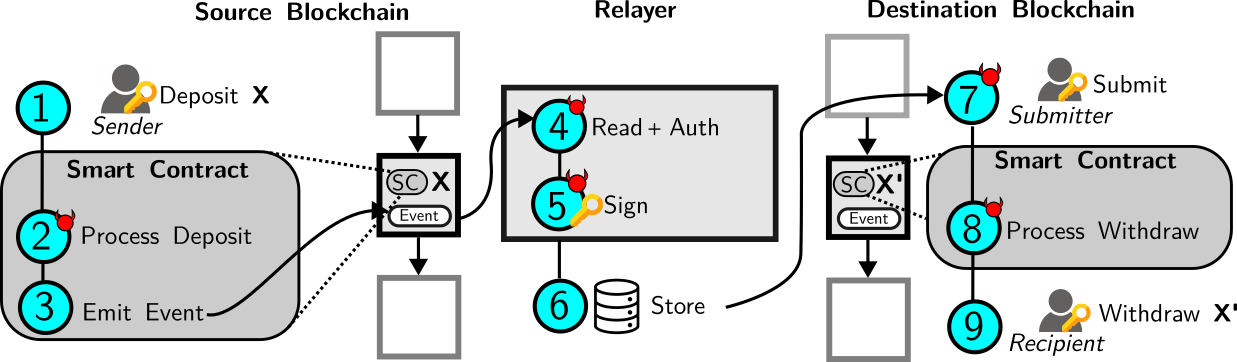
\includegraphics[width=0.8\textwidth]{fig/bridge_arch.pdf}
%%command for cropping pdf
%%gs -sDevice=pdfwrite -o bridge_arch_crop.pdf bridge_arch.pdf
\caption{Cross-chain token bridging and the different steps attackers can exploit to withdraw unbacked deposits.}
\label{fig:cross-chain}
\end{figure*}

\section{Background}
\label{sec:background}
% In this section, we start by providing an overview of blockchain technology. We then describe how cross-chain bridges work followed by the threat model we consider in this paper.
% In this section
We first give a brief introduction to smart contract blockchains
and cross-chain bridges. We then describe how bridges, under attack, collapse in
practice.

\subsection{Smart-contract Blockchains} Modern DeFi protocols (e.g.,
decentralized exchanges and lending protocols) are built on top
of ``smart-contract'' blockchains, like Ethereum. At their core, these chains, like
the original Bitcoin blockchain, are distributed ledgers that manage accounts
(public keys) and their balances (in native tokens like Ethereum's ETH). Users
interact with these chains by signing and broadcasting (to the distributed nodes
that make up the chain network) transactions that, for example, transfer
funds from their account (using the corresponding account private key) to
another user's account.

Ethereum, and the smart-contract chains it inspired since its release in 2015,
differ from Bitcoin by extending the ``simple'' distributed ledger with a smart
contract execution layer. A smart contract on Ethereum is an \emph{internal}
account---and, like a normal, \emph{externally owned} account (EOA), it has a
balance---that has associated \emph{code} (EVM bytecode), which implements the
smart contract's program logic, and \emph{storage}, which persists the program's
state across executions. Users interact with (i.e., execute) smart contracts
much like they do when transferring funds from their account: they sign a
transaction that encodes the smart contract to call (i.e., the contract address),
the particular function to execute, and the arguments to call the function with.
Instead of simply transferring funds from the user's account, then, executing
such a \emph{smart-contract call} transaction amounts to executing the smart
contract bytecode---and any smart contracts the contract itself calls.
    
% \begin{lstlisting}
% contract USDC{
%   mapping(account => amount) _balances;
%   event Transfer(from, to, value);
%   function transfer(to, amount) {
%     address from = msg.sender; // user
%     // ... validate user has enough balance
%     _balances[from] -= amount;
%     _balances[to] += amount;
%     emit Transfer(from, to, amount);
%   }

%   function mint(to, amount) {
%     _balances[to] += value;
%     emit Transfer(address(0), to, amount);
%   }

%   function burn(from, amount) {
%     // ... validate user has enough balance
%     _balances[from] -= amount;
%     emit Transfer(from, address(0), amount);
%   }

%   function safeTransferFrom(from, to, amount){ 
%     // ... transfer tokens; revert if failed
%   }
% }
% \end{lstlisting}


\begin{figure}[t]
    \centering
    \includegraphics[width=\columnwidth]{fig/usdc-contract-2sp.pdf}
    \caption{Simplified USDC ERC-20 Token Contract.}
    \label{fig:erc20}
\end{figure}


    

% \lstdefinestyle{myStyle}{
%     belowcaptionskip=1\baselineskip,
%     breaklines=true,
%     % frame=none,
%     % numbers=none, 
%     basicstyle=\footnotesize\ttfamily,
%     % keywordstyle=\bfseries\color{green!40!black},
%     % commentstyle=\itshape\color{purple!40!black},
%     % identifierstyle=\color{blue},
%     backgroundcolor=\color{gray!10!white},
%     language=Python,
% }

% \lstdefinestyle{customc}{
%   belowcaptionskip=1\baselineskip,
%   breaklines=true,
%   frame=L,
%   xleftmargin=\parindent,
%   language=Python,
%   showstringspaces=false,
%   basicstyle=\footnotesize\ttfamily,
%   keywordstyle=\bfseries\color{green!40!black},
%   commentstyle=\itshape\color{purple!40!black},
%   identifierstyle=\color{blue},
%   stringstyle=\color{orange},
% }


\subsection{ERC-20 Tokens}
One of the immediate applications of smart contracts---and to date still one of
most popular---is to create custom tokens (or coins).  To launch a new token, an
organization no longer needs to launch a new blockchain; they can instead deploy
a new contract that implements the ERC-20 token standard interface on a chain
like Ethereum and take advantage of existing on-chain infrastructure like
decentralized exchanges that make it easy to, for example, trade one kind of
token for another---both native tokens (e.g., ETH) and other tokens.\footnote{
    Most EVM chains, i.e., chains that use Ethereum's execution layer,
    follow Ethereum standards like ERC-20. Most non-EVM chains like Solana
    (which have different execution models) have similar standards (e.g., SPL
    tokens in Solana's case).
}

Figure~\ref{fig:erc20} shows a simplified variant of one such token
contract---the USDC \emph{stablecoin} contract.  This contract tracks
how many USDC tokens an account has and governs the spending of these
tokens (much like a bank governs bank notes).  For example, the
contract's \texttt{mint} function lets Circle (the company that owns
the USDC contract) mint new tokens into a user's account---e.g., after
receiving the corresponding payment from the user off-chain (in US
dollars, as USDC tokens are pegged to the US dollar).  The contract
exposes the ERC-20 interface that lets users (and smart contracts)
transfer tokens from their account by simply calling functions like
\texttt{safeTransferFrom}, and, in turn, use the tokens in any DeFi
protocol (e.g., lending the USDC to different markets, exchanging USDC
for ETH,
% buying NFTs using the USDC,
etc.). Finally, the contract's
\texttt{burn} function ``burns'' a token out of circulation---and
emits an event (Figure~\ref{fig:erc20-event}) that Circle's off-chain code looks for before allowing
a user to withdraw the corresponding USD fiat off-chain.

% \subsection{Blockchain Basics}
% In this section, we cover the basic concepts of blockchain technology, including blockchains, smart contracts, transactions, accounts, and tokens.

% \textbf{Blockchains.} A blockchain is a distributed ledger that stores data (e.g., account balance) in a transparent and tamper-proof manner. It consists of a chain of blocks, where each block contains a certain amount of data, a reference to the previous block (thus forming a chain), and other information such as timestamp. Blockchains are maintained by a network of nodes that validate data in the blocks and reach consensus on the state of the ledger.\alex{somehow have to mention Solana and Ethereum and others?}
% % It consists of a series of blocks that are linked together via cryptography (thus forming a chain) [65]. These blocks are immutable and can be used to store data (e.g., transactions). They are also maintained by a distributed network of nodes, removing the need of a central server. 

% \textbf{Smart Contracts.} Smart contracts are programs that can be executed. Typically, smart contracts are first written in high-level programming languages such as Solidity or Rust. Then, they are compiled into bytecode and deployed to the blockchain. Upon deployment, each smart contract is assigned a unique address and becomes immutable. After deployment, they can be executed based on the input provided and the logic programmed into the contract.

% % , compiled into bytecode, and deployed to the blockchain. The input and execution of smart contracts are all recorded on the blockchain. They 

% % are stored and executed on blockchains. They are used to encode business logic, enforce rules, and automate processes. Smart contracts are written in high-level programming languages, compiled into bytecode, and deployed to the blockchain. Once deployed, smart contracts are immutable and can be interacted with by sending transactions.

% % self-executing programs that run on blockchains. They are used to encode business logic, enforce rules, and automate processes. Smart contracts are written in high-level programming languages, compiled into bytecode, and deployed to the blockchain. Once deployed, smart contracts are immutable and can be interacted with by sending transactions.

% \textbf{External Owned Accounts.}  Externally owned accounts (EOAs) represent users and are controlled by private keys. Users can interact with other users or deployed smart contracts by initiating a transaction from their EOAs. To initiate a transaction, a user specifies the recipient (the address of an EOA or a smart contract), the amount of assets to transfer, and any additional input parameters required by the smart contract. 

% % are entities that can send and receive transactions on the blockchain. There are two types of accounts: externally owned accounts (EOAs) and contract accounts. EOAs are controlled by private keys and represent human users, while contract accounts are controlled by smart contracts and represent autonomous entities.

% % Accounts are entities that can send and receive transactions on the blockchain. There are two types of accounts: externally owned accounts (EOAs) and contract accounts. EOAs are controlled by private keys and represent human users, while contract accounts are controlled by smart contracts and represent autonomous entities.


% \textbf{Transactions.} A transaction is a instruction set constructed and signed by a user using their EOA. It typically includes several fields, such as the sender (the EOA that signs the transaction), the recipient (which can be an EOA or a smart contract), the amount of assets to transfer, and the input parameters required by a smart contract. Once signed, the transaction is broadcasted to the network and executed. After successful execution, the resulting state changes are recorded on the blockchain along with the transaction itself.


% \textbf{Tokens.} Every blockchain system has its own native token. For example, Ethereum has Ether (ETH), while Solana has Sol (SOL). In addition to native tokens, blockchains can also host other types of tokens. An example is ERC-20 tokens on Ethereum, which are smart contracts that follow a set of rules and standards. Of particular note, when a user transfers ERC-20 tokens, the ERC-20 token contract emits an event (a type of debug information recorded on the blockchain) that logs certain information. Figure 1 shows an example. The name of the event is Transfer, and the token contract that emits the Transfer event is tagged as USDC. The sender and recipient are represented by their addresses (0x68... and 0xF5..., respectively). The amount of tokens transferred is 212295874.

% \alex{maybe liquidity pool}


\subsection{Cross-Chain Token Bridges}
While smart contracts make it easy to launch new tokens without spinning up new
chains, there is no real shortage of new blockchains being deployed (almost weekly).  Indeed,
the modern blockchain ecosystem is a many-chain ecosystem.  Blockchains like
Avalanche, Base, and Solana have different design points---from cheaper ``gas''
execution costs, to higher throughput, lower latency, and different permission
models---that make them better suited for different classes of application.
This situation has resulted in applications that span many chains and cross-chain
infrastructure that ultimately (try to) allow users to, for example, buy
Dogwifhat NFTs on Solana using USDC tokens on Ethereum.

Core to these applications and infrastructure---and the focus of our work---is
the \emph{cross-chain token bridge}.  At a high level, a cross-chain token
bridge makes it possible for a user to ``transfer'' their tokens from one chain
(e.g., their USDC on Ethereum) to another chain (e.g., Solana) and then use the
transferred tokens on the destination chain (e.g., on a Solana exchange trading
USDC and Dogwifhat).\footnote{While some cross-chain bridges \emph{do} let users
transfer one kind of token (e.g., USDC on Ethereum) for a completely different
kind of token on the destination chain (e.g., Dogwifhat on Solana), these bridges
essentially fuse the cross-chain token bridge with an exchange (or swap). We
focus on token bridges not only because they are fundamental to other kinds of
bridges, but also because they have higher volume, more liquidity, and more
attacks.} Since smart contracts cannot make network requests or otherwise
access sate outside their own storage, a cross-chain token bridge consists of
smart contracts on both the source and destination chains, and off-chain
infrastructure that serves to relay the ``transfer'' call across the two
contracts.

\begin{figure}[t]
\centering
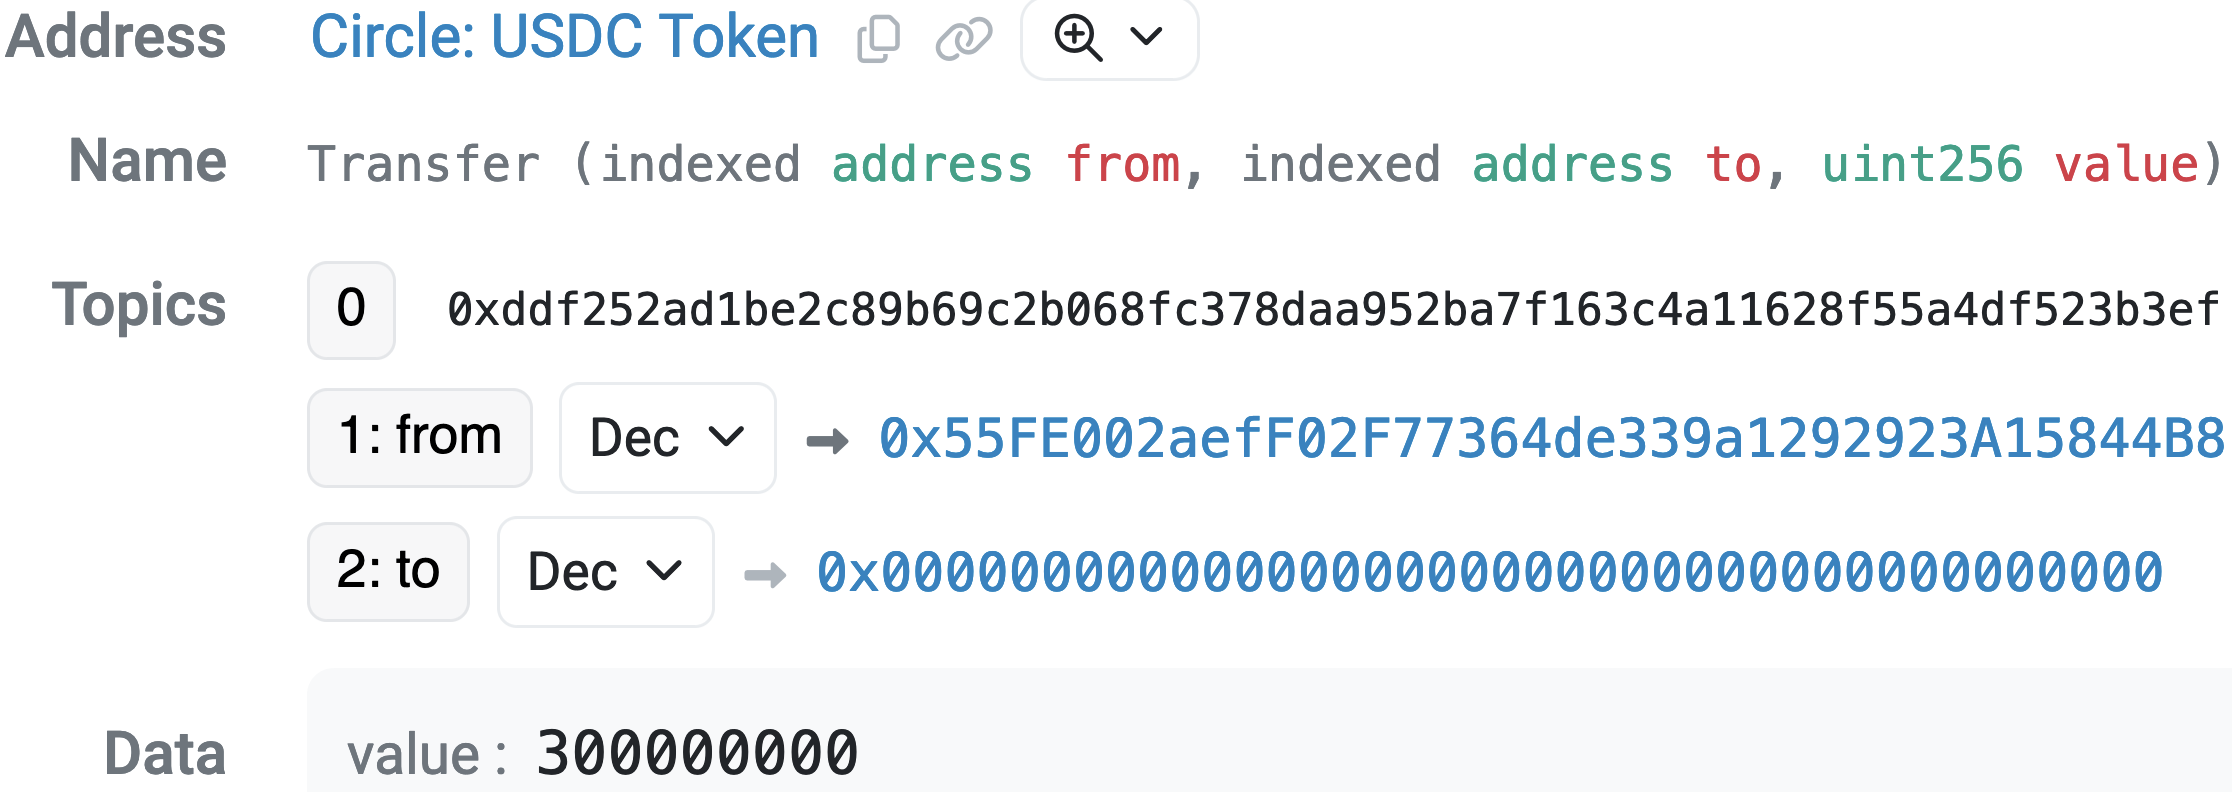
\includegraphics[width=\columnwidth]{fig/token.png}
\caption{Event Emitted by an ERC-20 Token (USDC).}
\label{fig:erc20-event}
\end{figure}

As Figure~\ref{fig:cross-chain} shows, a typical cross-chain token transfer,
i.e., a bridge transaction, consists three phases:

\textbf{1. Deposit (on source chain).}
To initiate a cross-chain token transfer, the user first calls the bridge's
contract on the source chain:
\begin{lstlisting}
deposit(address token, uint256 val, address to) {
  address from = msg.sender;  // user
  address to = address(this); // bridge contract
  // ... validate the ERC-20 token contract
  token.safeTransferFrom(from, to, val);
  emit Deposited(id++, token, from, to, val);
}
\end{lstlisting}
This contract function---a simplified version of the Qubit bridge deposit
function---processes the user's deposit (step 2) by validating the transfer request,
e.g., against a list supported tokens, and then transferring the user's ERC-20
tokens to the bridge contract---recall contracts are accounts with balances.
Then, the function emits an event (step 3) recording the user's deposit details
(including the deposit ID, the ERC-20 token contract address, the recipient on
the destination chain, and value).

\textbf{2. Off-chain relay.}
The emitted event is observed by an off-chain relayer in (step 4),
which constantly monitors the source blockchain.  The relayer first
verifies the authenticity of the deposit event.  If the event is
authentic, the relayer then produces a signed \emph{receipt}
endorsing the deposit (step 5) and, typically, stores the receipt off-chain (step
6).  Finally, this signed receipt is sent to the bridge's withdrawal contract
on the destination blockchain (step 7). Who submits the receipt varies across
bridges---some bridges submit the receipt on the user's behalf (in these cases, the
signed receipt is simply a signed contract-call transaction), while others give
users (and anyone willing to pay gas) the signed receipt and they, in turn,
submit the receipt to the withdrawal contract to complete the transfer. 

\textbf{3. Withdraw (on destination chain).}
The withdrawal contract on the destination chain first processes the withdraw
request by verifying the receipt and transferring the tokens to the recipient
(step 8). In (the simplified) Chainswap's withdraw case, for example, users call:
\begin{lstlisting}
withdraw(uint256 id, address token, address to, uint256 val, Signature[] sigs) {
  _chargeFee();
  // verify receipt
  require(received[id][to] == 0, 'withdrawn');
  for(uint i=0; i < sigs.length; i++) {
    verify_receipt(sigs[i], id, token, to, val);
  }
  received[id][to] = val; // mark as withdrawn
  token.safeTransferFrom(address(this), to, val);
  emit Withdraw(id, token, to, val);
}
\end{lstlisting}
This contract function first charges the caller a fee, then verifies the
deposit details against receipt---both that the deposit was not already
withdrawn and that the receipt signatures are valid---and finally transfers the
tokens to the intended recipient.  We consider a cross-chain transaction
complete when the asset is released to the recipient (step~9).

We expect every cross-chain bridge transaction to uphold the balance invariant:
the value (and kind) of the tokens withdrawn---the outflow---should equal the
value (and kind) of the tokens deposited---the inflow---minus the charged fees.
In practice, they do not.



% \subsection{Cross-Chain Bridges}
% In this section, we begin by providing an example of how a typical cross-chain transaction works. We then discuss the different variants of cross-chain bridges. 
% \subsubsection{A Typical Cross-Chain Transaction}
% Figure~\ref{fig:cross-chain} depicts a typical cross-chain transaction. Starting with the source blockchain, the sender (represented by their EOA) initiates a transaction to transfer assets to the bridge's deposit contract (step 1). The bridge contract then verifies that it has received the assets (step 2). Upon verification, the bridge contract emits an event to record the transfer (step 3). This event is observed by the relaying component (step 4), which typically resides outside and constantly monitors the source blockchain. The relaying component then verifies the authenticity of the event (step 5). If the event is authentic, the relaying component signs the message and stores the signature in a queryable database (step 6). A submitter on the destination blockchain then fetches the signed message from the database (step 7) and sends it to the bridge's withdrawal contract on the destination blockchain (step 8). The bridge contract then verifies the signature (step 9) and transfers the assets to the recipient (step 10). A cross-chain transaction is considered complete when the asset is released to the recipient (step 11).

% % Important things we need in this figure:
%     % source and dst amount
%     % how different vulnerabilities manifest
%         % source
%             % transfer in
%             % verify * emit
%         % relaying component
%             % observe
%             % signs
%         % dst
%             % retrieve & send
%             % verify
%             % transfer out
%     % Players
%         % Sender (in source)
%         % Relayer (in dst)
%         % Receiver (in dst)
    
    



% \subsubsection{Variants of Bridge Implementation}
% Beyond the typical cross-chain transaction described above, there are different ways to implement a cross-chain bridge. We discuss the following variants:

% \textbf{Asset Management.} There are two common ways funds can be released in step 10. The first model is the liquidity pool, which is commonly used when an asset already exists on both blockchains (e.g., USDC already exists on Ethereum and Polygon). Bridges start by creating liquidity pools, to which users can deposit assets and earn fees. When a withdrawal request is made, the bridge releases the funds from the liquidity pool as long as there is sufficient capital in the pool. The second model is mint-and-burn, which can be used regardless of whether the asset exists on the destination blockchain. In this model, the bridge contract mints new tokens on the destination blockchain, which act as representations of the assets on the source blockchain. When a withdrawal request is made, the bridge simply mints new tokens and sends them to the recipient. The recipient can then burn the tokens to receive the original assets on the source blockchain.



% \textbf{Submitter Privilege.} In the flow depicted in Figure~\ref{fig:cross-chain}, once the relaying component has signed the transaction, anyone can fetch the signed message and submit it to the destination blockchain. However, in practice, there is a variant where only privileged EOAs can act as submitters. In this variant, the authenticity of the message is verified by the presence of a privileged key. If bridges choose to operate in this way, they 
% typically simplify step 6 by directly storing the message without signing it.

% \textbf{Transaction Relay.} In the flow depicted in Figure~\ref{fig:cross-chain}, each transaction is relayed individually. In practice, transactions can also be relayed in batches or grouped into a Merkle tree. This approach can improve efficiency. However, while using a Merkle tree is more efficient, it also introduces additional complexity in step 9, where the bridge contract has to verify that a transaction is included in a Merkle tree.

% \textbf{Message Verification Mechanisms.} There are four different mechanisms to verify the authenticity of a message. Namely, external verification, optimistic verification, native verification, and local verification. The details of these mechanisms are not critical for this paper. We provide a brief overview of each model and refer the reader to \alex{cite} for more details. At a high level, external verification indicates that the relaying component resides outside both the source and destination blockchains. The legitimacy of a cross-chain transaction is attested by a third party (or a set of third parties). Native verification, on the other hand, indicates that the relaying component resides within the destination blockchain. In this model, the relaying component typically operates as a light client of the source blockchain and maintains enough information to verify the authenticity of a message from the source blockchain. Optimistic verification improves the efficiency of external verification by assuming that the majority of relayed transactions on the destination blockchain are valid. Instead of attesting to the validity of every transaction, optimistic verification only intervenes when a fraudulent transaction is detected. Finally, local verification means that the two parties involved in a cross-chain transaction (e.g., the sender and the submitter) must cooperate and collaborate for the transaction to succeed.

% \textbf{Token Swap Bridges.} In the above example, tokens released on the destination blockchain are backed by an equivalent amount of assets (less fee) on the source blockchain. However, in practice, bridges can also support token swap. In this case, an asset on the source blockchain is swapped for a different asset on the destination blockchain. For example, a user can swap 1 ETH for 100 USDC. The conversion rate is typically determined by the relaying component and may not be publicly disclosed. 

% \subsubsection{Variants of Verification Mechanism.}
% \textbf{External Verification.} In the most common case, the verification components resides outside both the source and destination blockchains. This is known as an externally verified bridge. The legitimacy and correctness of a cross-chain transaction is determined by a third-party (or a set of third-parties). Common ways to implement external verification include Multi-party Computation and Threshold Signature Scheme.\alex{cite}

% \textbf{Optimistic Verification.} Optimistic Verification improves on the efficiency of external verification by assuming that the majority of transactions are valid. Instead of attesting to the validity of every transaction, optimistic verification only intervenes when a dispute arises. This is known as an optimistic bridge. Concretely, every message that is passed to the destination blockchain is considered "pending" until the dispute window expires. The system relies on one or more honest watchers to dispute the message if it is incorrect. If no dispute arises, the message is considered valid.

% \textbf{Native Verification}
% Contrary to external verification, where the verification component resides outside the source and destination blockchains, the verification component in a natively verified bridge resides within the destination blockchain. Commonly, this is achieved by implementing a light client of the source blockchain within the destination blockchain, which maintains enough information for verifying the authenticity of a message. The security is guaranteed by the validators of the source chain. 


% \textbf{Local Verification}
% \alex{add citation. this is the most confusing one.}
% The basic idea is that the sender and the submitter
% have to cooperate and collaborate for a cross-chain transaction to succeed. 

\subsection{How Bridges Collapse}
In practice, attackers exploited bugs in all three components---the deposit
contract, the relayer, and the withdraw contract---and stole signing keys
to siphon hundreds of thousands of dollars.
%
Figure~\ref{fig:cross-chain} highlights the precise steps in the cross-chain
token transfer that attackers have historically exploited, including:
\begin{CompactItemize}
\item \textbf{Bugs in the deposit contract.} In step 2, the bridge contract
verifies that it has received the correct amount of assets before emitting an
event. Bugs in this verification logic could allow an attacker to deposit a
smaller amount of assets than what is recorded by the bridge in the event (step
3). For example, Qubit's \texttt{deposit} function  (see above) did not properly validate the token address. This bug allowed an attacker to pass \texttt{0} for the token address, so the contract function did not actually transfer any funds from the attacker's account but still emitted a \texttt{Deposit} event which allowed the attacker to withdraw actual tokens on the destination chain~\cite{qubit:rekt}.

\item \textbf{Bugs in the off-chain deposit verification.} In step 5, the
relayer verifies the authenticity of the deposit event emitted by the
bridge contract, including whether the event is emitted by the bridge's
designated contract.  Bridges that do not correctly verify
deposits would allow attackers to withdraw assets that are never deposited.
% ---and this 

\item \textbf{Stolen relayer (or submitter) keys.} In step 5, the relayer signs the deposit receipts which are then submitted to the withdrawal
contract as evidence of a valid deposit. If the relayer key is compromised
(e.g., as with the Ronin bridge~\cite{roninattack}) the attacker can forge a
valid receipt and then withdraw assets that were never deposited by calling
\texttt{withdraw} with the forged receipt.

The same is true for bridges that submit receipts on behalf of users---and
essentially restrict the \texttt{withdraw} callers to privileged submitter
accounts. The bridge submitter keys (step 8) have similarly been compromised
(e.g., as with AnySwap~\cite{anyswapattack}) and used to withdraw
unbacked deposits.

\item \textbf{Bugs in the withdraw verification.} In step 8, the bridge contract
verifies that the messages are signed by the relayer and have not
been replayed. Bugs in this verification logic (e.g., as we saw with
Wormhole~\cite{wormholeattack}) have allowed attackers to supply ``valid''
payloads that were not signed by the relayer and replay withdrawal
requests with valid deposit receipts that have already been withdrawn.
\end{CompactItemize}


% Liquidity Pool vs Mint-and-Burn. Example USDC on ETH and Polygon
% Verification Modes
% \subsection{Threat Model}
% In this section, we describe the attack surfaces that are in scope for this paper. Importantly, we assume that deposits and withdrawals are made through designated functions and that funds cannot be withdrawn through functions other than the designated withdrawal function(s). Given this setup, we consider the following attack surfaces:

% \textbf{Buggy Deposit Verification.} In step 2, the bridge contract verifies that it has received the correct amount of assets before emitting an event. Bugs in this verification logic could allow an attacker to deposit a smaller amount of assets than what is recorded by the bridge in the event (step 3).

% \textbf{Buggy Event Verification.} In step 5, the relaying component verifies the authenticity of the event emitted by the bridge contract, including whether the event is emitted by the bridge's designated contract. Failure to do so could allow an attacker to withdraw assets that were never deposited.

% \textbf{Compromised Relaying Key.} In step 6, the relaying component signs the message and stores the signature in a queryable database. If the relaying key is compromised, an attacker could forge a message and withdraw assets that were never deposited.

% \textbf{Compromised Submitter Key.} In step 8, some bridges operate in a privileged submitter mode, where the presence of the privileged submitter key is the only requirement to attest to the authenticity of a message. In this case, if the submitter key is compromised, an attacker could submit a forged message and withdraw assets that were never deposited.

%\textbf{Buggy Withdraw Verification.} In step 9, the bridge contract verifies that the messages are signed by the relaying component and have not been replayed. Bugs in this verification logic could allow an attacker to verify payloads that are not signed by the relaying component or to replay a message that has already been processed.

In this paper, we assume an attacker can exploit any of the aforementioned
components or otherwise control the relayer (or submitter) keys.
In the next section, we show that this attacker model and our simple
\emph{balance invariant checking} captures the largest attacks on cross-chain
bridges that have happened in the past.  In Sections~\ref{sec:live-audit} we show
that monitoring withdrawals and deposits on the source and destination chains
can be used to detect similar attacks in the future.  Finally, in
Section~\ref{sec:active-protect} we describe an \emph{announce-then-execute} bridge
design that enforces this invariant to prevent attacks before they happen.

We note that while our threat model captures a wide variety of vulnerabilities,
it is not exhaustive.  As with any detection system, an attack that violates one
of our assumptions (e.g., avoids violating the balance invariant by transferring
funds off-bridge or not having a withdrawal, subverts the transaction data used to validate the invariant,
etc.) might succeed.  
We similarly consider other smart contract bugs (beyond bugs in deposit and withdrawal functions) and account key compromises out of scope---and instead focus
on the cross-chain bridging aspects which are relatively less well understood.
As we show later, our model captures the largest attacks on
cross-chain bridges that have happened in the past and systems can use
it to prevent similar attacks in the future.


%% While our approach captures a variety of vulnerabilities, it is by no
%% means exhaustive. For example, a key assumption we make is that
%% withdrawal are done through designated withdraw functions. However, if
%% an adversary is able to compromise the key to account that holds the
%% funds for the bridge, they could simply transfer the funds to another
%% account and then withdraw them without going through the designated
%% withdraw function(s). Similarly, if an adversary is able to withdraw
%% funds by repurposing other functions (e.g., the deposit function), our
%% approach would not detect it. Moreover, if an attack transaction does
%% not involve a withdrawal, our approach would not detect it. Last but
%% not least, if an attack is somehow able to profit without breaking the
%% balance invariant, our approach would not detect it.  However, we
%% believe that our approach is a important first step in using
%% accounting principles to protect bridges from theft and that it can be
%% extended to address these and other vulnerabilities in the future.


%\section{The Invariant}
\alex{Describe the invariant here (using source and dst).}
We observe that for token transfer bridges—those that facilitate the transfer of tokens between blockchains without performing token swaps—the inflow and outflow of tokens should be equivalent after factoring in fees. In other words, the outflow should be strictly less than or equal to the inflow due to the presence of fees. I refer to this principle as the invariant.


Below, I describe how the various attacks violate the invariant. For buggy deposit verification, an attacker deposits less than the amount withdrawn, resulting in a scenario where outflow exceeds inflow. For buggy event verification, compromised relaying key and compromised submitter key, the attacker withdraws assets that were never deposited, resulting in a scenario where inflow is zero and outflow is non-zero. For buggy withdraw verification, if the attacker can verify arbitrary payload, then the inflow is zero and outflow is non-zero. If the attacker can replay a message, then the inflow is non-zero and outflow is greater than inflow. In summary, in all cases, the invariant is in that the outflow is strictly greater than the inflow, rather than equal to or less than the inflow.

\alex{has been done at a grand scale}

\alex{add a figure to illustrate the invariant.}


\section{Approach}
\label{sec:meth}

The core hypothesis of our work is that value should be conserved
within cross-chain transactions.  That is, that the value of the asset
inflow in such a transaction (i.e., the deposit) should equal the
value of the asset outflow (i.e., the withdrawal).  In token transfer
bridges, this invariant corresponds to a balancing of the inflow
tokens and the outflow tokens (less any fees or transaction costs
incurred by the bridge itself).  When this balance invariant does not
hold it allows a range of opportunities for fraud, all of which
involve greater outflows (withdrawals) than inflow
(deposits). Figure~\ref{fig:invariant} illustrates such an outcome by 
graphing the \emph{aggregate} difference between bridge inflow (on
Ethereum) and outflow (on Solana) leading up to and during the
February 2022 attack on the Wormhole bridge.  The net difference is
consistently near zero, with only short positive deviations
(representing delayed withdrawals) until the attack in January, at
which point there are significant withdrawals without matching
deposits---producing a large negative difference.

Testing this invariant on a \emph{per transaction basis} is
straightforward in principle. However, since bridge transaction formats are
not standardized, it requires a range of per-bridge and per-chain
parsing in practice.  Our methodology for normalizing this information
focuses on two key pieces of information: a) identifying each bridge
transaction---a composite of a deposit (inflow) transaction on a
source blockchain and a withdrawal (outflow) transaction on
another---and b) identifying the value transferred in each such bridge
transaction.

\begin{figure}[t]
  \centering
  \includegraphics[width=0.7\columnwidth]{fig/sec25_plot_wormhole.pdf}
  \caption{Total Inflow (on Ethereum) - Total Outflow (on Solana) Over Time: Wormhole Attack in Feb 2022.}
  \label{fig:invariant}

\end{figure}


\subsection{Identifying Bridge Transactions}
For almost all bridges, identifying their component (per-chain) inflow
and outflow transactions is straightforward --- bridges typically use
explicit events on each chain to signal if a given transaction is a
deposit or withdrawal.\footnote{One key exception to this rule is the
  Wormhole bridge which, until late 2023, did not emit specific
  events when executing a withdrawal transaction.  In this case, we infer that a withdrawal took
  place by looking for transactions that invoke functions designated for performing withdrawal operations (e.g., \textit{completeTransfer}).
  %have synthesized such an event ourselves by parsing the function
  % names called by the transaction to .  
  It also appears to be widely understood today that emitting
  explicit events is a best practice.}

Pairing these component transactions (i.e., matching deposits on one
chain to withdrawals on other) can be performed in several different
ways.  The easiest, and most common, is via a unique transaction
identifier. Such IDs are typically generated by the bridge on the
\emph{source chain} during a deposit transaction and then copied into
the withdrawal transaction on the destination chain.\footnote{These
  unique IDs are commonly simple global variables incremented with
  each new transaction.}  However, instead of an explicit ID, some
bridges use a hash of the deposit transaction for the same purpose
(e.g., for Anyswap, each withdraw transaction will include the hash of
its corresponding deposit transaction).\footnote{We note that to prevent potential replay attacks, bridge implementers should also include an ID that uniquely identifies individual deposit events within a transactions. Sadly, this is often not the case.}  Finally, in a handful of cases there are
no ``inband'' identifiers that can be used to associate transactions.
We believe this is a poor design choice that is fundamentally in
conflict with auditability.  However, even in these cases, for the
purpose of our analysis we have been able to pair transactions using
explicit query APIs provided by the affected bridges
services.\footnote{For example, when a bridge transaction on the Poly
  Network bridge includes a withdrawal from Curve (a kind of liquidity
  pool) or when a bridge transaction on the Binance Token Hub includes
  a Binance Smart Chain (BSC) withdrawal, it is not possible to
  identify the partner deposit from blockchain data alone and we must
  make use of ``out of band'' data available through their respective
  bridge query APIs.}

  At the end of this process, we identify a comprehensive collection
  of ``bridge transactions'' (a pair of transactions from two
  different blockchains that were used by the bridge to transfer
  value across them). While the vast majority of bridge transactions
  are pairs of deposit and withdrawal transactions, a handful of
  bridge transactions are either withdrawal-only (e.g., in the case of
  attacks) or deposit-only (e.g., if the user chooses to delay their
  withdrawal).

% And for 
% a handful of bridge transaction, they are either withdrawal-only or deposit-only, and we treat them as singleton transactions.
%  and a handful of singleton
% transactions (i.e., which involve the bridge, based on their
% addresses, but are withdrawal-only or deposit-only).


%For example, with the Binance bridge, the matching transaction for a BSC transaction can only be identified by querying the API. 
%%% here.
%Similarly, for Poly Network bridge, when users withdraw from Curve (a kind of liquidity pool), the matching deposit amount is not recorded on the blockchain, as its a special type of withdrawal where the matching deposit is computed off-chain and only available through the API. In this case, we also rely on Poly Network's API to pair the deposit and withdraw transactions, if the deposit transaction is from Curve. \elisa{It might be nice to give a reason why the pairing info is not available for these cases if we know.} 




%\textbf{Using Unique ID.} Most of the bridges\alex{how many?} will create a unique id for each deposit transaction (incrementing by 1).
%A withdraw transaction will contain this unique id. We can then use this unique id to pair the deposit and withdraw transactions.



%\textbf{Using the transaction hash of the deposit transaction.}
%Another way to pair deposit and withdraw transactions is to use the transaction hash of the deposit transaction. A withdraw transaction will include the transaction hash of the corresponding deposit transaction hash. We can then use this information to pair the deposit and withdraw transactions.

%\textbf{Using the official API.}
%Some bridges provide APIs to query matching deposit and withdraw transactions. While this feature mostly exist for user convenience, sometimes we have to rely on this API to pair deposit and withdraw transactions, as the pairing information is not directly available as part of the withdraw transaction.\alex{maybe we should hedge here and say its not trivial to get the information.} 
%For example, with the Binance bridge, the matching transaction for a BSC transaction can only be identified by querying the API. 
%%% here.
%Similarly, for Poly Network bridge, when users withdraw from Curve (a kind of liquidity pool), the matching deposit amount is not recorded on the blockchain, as its a special type of withdrawal where the matching deposit is computed off-chain and only available through the API. In this case, we also rely on Poly Network's API to pair the deposit and withdraw transactions, if the deposit transaction is from Curve. \elisa{It might be nice to give a reason why the pairing info is not available for these cases if we know.} 

\subsection{Identifying the Value Transferred}
Many bridge transaction event formats explicitly identify the amount
and kind of tokens transferred. However, some bridges do not emit this
information and others can be unreliable.\footnote{For example, as
  mentioned earlier, pre-2024 Wormhole does not emit an event for
  withdrawal transactions. Other examples include the Meter bridge and
  Qubit bridge, which attempted to verify the number of tokens
  received but had exploitable bugs.}  In such cases, we can
frequently make use of the ERC-20 ``Transfer'' event (see
Figure~\ref{fig:erc20-event} for an example) that is emitted when the
contract transfers the tokens from the user's account to the bridge's
account.  This event contains the number of tokens transferred as well
as the sender and recipient addresses, which we use to identify the
number of tokens transferred to or from the bridge.  Because the
Transfer event is adjacent to its associated bridge-generated event,
it is easy to identify and thus establish the number of tokens
transferred.\footnote{As a sanity check, we also require that the
  sender and recipient addresses in the Transfer event are consistent
  with the bridge's defined behavior: for withdrawal transactions, we
  require that the sender is either a mint address (i.e., all-zero
  address) or a bridge-controlled address, while for deposit
  transactions, we require that the recipient is either a burn address
  (i.e., all-zero address) or a bridge-controlled address.}  In a few
implementations, multiple related Transfer events can be emitted at
once, and in these cases we have manually inspected their contracts
and constructed implementation-specific logic to account for this
behavior.  Another special case is caused by so-called ``reflection
tokens'' in which the number of tokens logged in the event (the value
field in Figure~\ref{fig:erc20-event}) is dynamically adjusted based
on a combination of the intended number and the total token supply.
For such cases, we either rely on bridge events which capture the
intended number of tokens transferred or implement token-specific
logic to recompute the value accordingly.  Finally, native tokens have
no Transfer event (since they are not ERC-20 tokens), but thus far we
have either been able to recover the number of tokens transferred from
bridge events or so-called ``internal transactions''.

To summarize, while it is certainly possible to create a bridge
transaction protocol that records insufficient data to match deposits
and withdrawals, or for which the number of tokens transferred might
be ambiguous, our empirical experience analyzing 11 bridges and 21
blockchains is that such reconstruction has always been possible.


%When the amount of tokens transferred logged by the bridge is unavailable or unreliable, we can use the Transfer event emitted by an ERC20 token contract to identify the amount of tokens transferred. The Transfer event, part of the ERC20 standard, has been used by prior research in other scenarios.\alex{cite} This event contains the amount of tokens transferred as well as the sender and recipient addresses, which we use to identify the amount of tokens transferred to or from the bridge. Concretely, we observe that for any successful bridge transaction, depending on the order of execution, the transfer event either happens right before or after the bridge-generated event. As a result, we can first locate the bridge event and then look for the Transfer event that happens right before or after the bridge event, which contains the amount of tokens transferred. As additional sanity checks, we also require that the sender and recipient addresses in the Transfer event are consistent with the bridge's behavior. Namely, for withdraw transactions, we require that the sender is either a mint address (e.g., all-zero address) or a bridge controlled address. On the other hand, for deposit transactions, we require that the recipient is either a burn address (e.g., all-zero address) or a bridge controlled address.\alex{do we have to explain the intuition?}


%There are two ways to identify the amount of tokens transferred by the bridge: using the amount logged in a 
%bridge-generated event or using the Transfer event emitted by ERC20 tokens. Specifically, some bridges include the amount of tokens sent or received in their events. However, this information is not always reliable, as bridges can have bugs (typically when they don't verify the amount of tokens they actually received), which is the case for [AL: which]. Additionally, some bridges do not emit this information. In such cases, we can use the token transfer event to identify the amount of tokens transferred, which also serves as the ground truth.

%\textbf{Identifying Token Transferred from Transfer Event.} 
%When the amount of tokens transferred logged by the bridge is unavailable or unreliable, we can use the Transfer event emitted by an ERC20 token contract to identify the amount of tokens transferred. The Transfer event, part of the ERC20 standard, has been used by prior research in other scenarios.\alex{cite} This event contains the amount of tokens transferred as well as the sender and recipient addresses, which we use to identify the amount of tokens transferred to or from the bridge. Concretely, we observe that for any successful bridge transaction, depending on the order of execution, the transfer event either happens right before or after the bridge-generated event. As a result, we can first locate the bridge event and then look for the Transfer event that happens right before or after the bridge event, which contains the amount of tokens transferred. As additional sanity checks, we also require that the sender and recipient addresses in the Transfer event are consistent with the bridge's behavior. Namely, for withdraw transactions, we require that the sender is either a mint address (e.g., all-zero address) or a bridge controlled address. On the other hand, for deposit transactions, we require that the recipient is either a burn address (e.g., all-zero address) or a bridge controlled address.\alex{do we have to explain the intuition?}

%\textbf{Additional Considerations.}
%We note a few additional considerations. First, while the transfer action usually results in a single event, there are cases where multiple Transfer events are emitted. In such cases, we need to incorporate token-specific logic to capture a series of Transfer events to identify the amount of tokens transferred. For tokens exhibiting this behavior, we manually examine their code and account for their logic in our analysis.
%Next, for transfers involving native tokens, the value sometimes is included in internal transactions, and no event is emitted. We use the internal transactions to identify the amount of tokens transferred. Lastly, for a special type of tokens called reflection tokens, we need to account for the reflection mechanism. Specifically, reflection tokens have a mechanism where the real amount of tokens transferred is dynamically adjusted based on intended amount and total supply. For some tokens, they emit events that include enough information to recompute the intended amount. We thus use this information to identify the intended amount of tokens transferred. For other tokens, they do not provide such information. However, for those cases, conveniently, the bridge event includes the intended amount of tokens transferred. We thus revert back to use the amount logged by the bridge.\footnote{The delta between the intended amount and the real amount is very small (typically within a factor of 0.01). Thus, even if the initial amount is not logged by the bridge, the intended amount can still be bounded.}

\subsection{Checking the Balance Invariant}
Once we have identified both sides of the bridge transaction and the
number of tokens transferred by the bridge, we can verify if the
balance invariant holds: for each bridge transaction (including those
that are withdrawal-only), does the number of tokens transferred from
the bridge---the withdrawal amount---match the number of tokens
received by the bridge---the deposit amount?

However, a key complication is that bridges can charge fees and, while
these fees can sometimes be paid ``out of band'', it is not uncommon
for them to be subtracted from the tokens received on deposit.  To
account for this behavior (i.e., outflow = inflow - costs), we must be
able to determine such costs on a per-transaction basis.
In most cases, fees can be accounted for in a straightforward manner:
they either are made explicit in bridge-generated events (and can thus
be accounted for directly) or can be calculated based on either
published fee schedules or inferred fee schedules (i.e., since all
transactions are typically subject to the same fixed or percentage
fees).


%In practice there are two (additional) factors that influence this
%calculation. First, tokens could have different decimals on different blockchains.
%We account for this difference by retrieving the token's decimal information on each blockchain
%and normalizing the amount of tokens transferred accordingly. More concretely, token transfer values are expressed in the smallest unit of the token.

%\deian{dont use passive voice---who expresses them?} As an example, for a token with 6 decimals, 1 token = $10^6$ units. For the amount $212295874$ in Figure~\ref{fig:erc20-event}, if the token has 6 decimals,
%the normalized amount of tokens (also known as the whole unit amount) transferred to $212295874 / 10^6 = 212.295874$. 
% this by... XXX alex... I don't understand the sentence ``by using
% the token's decimal information to normalize the amount of tokens
% transferred''.

%.  In others, they may not be reported, but
% can be calculated based on either published fee schedules or inferred
% fee schedules (i.e., since all transactions are typically subject to
% the same fixed and percentage fees).

In some cases, the precise value of fees may be difficult to determine
retrospectively because they depend on some external contemporaneous
value not recorded in the transaction (e.g., fees valued in US dollars
implicitly depend on the exchange rate of a given token at that time).
While such ambiguity could be further minimized with additional data,
in our work we manage this issue by defaulting to a simple rule
that the number of tokens withdrawn should not exceed the number
deposited.






%We note a few additional considerations here. First, we note that the amount typically includes decimals, and the same token can have different number of decimals on different blockchains. We account for this by using the token's decimal information to normalize the amount of tokens transferred. Next, for some bridges, the amount of tokens transferred is not equal to the amount of tokens received because of the bridge fee. We address this issue by using the fee information provided by the bridge. When the fee information is unclear or specified in real currency (e.g., US dollars), we simply require that the amount of tokens transferred is less than or equal to the amount of tokens received by the bridge. 




\begin{facingcaption}{table}
\caption[The Blockchains \offlinetool Supports and the Cross-chain Bridges that Operate on Them.]{The blockchains \offlinetool supports and the cross\-chain bridges that operate on them.  While a particular attack on a
    bridge involves two chains, I collect deposit and withdrawal
    transactions for a bridge on all chains that the bridge supports. Anyswap is also known as Multichain.}
\label{table:chain_bridge_full}
\renewcommand\tabularxcolumn[1]{>{\RaggedLeft\arraybackslash}p{#1}}
\parindent=0pt
\setbox0=\vbox{%
\vsize\textwidth
\hsize\textheight
\linewidth\hsize
\columnwidth\hsize
\textwidth\hsize
\textheight\vsize

\begin{tabular}{ll}
  \toprule
  \textbf{Blockchain} & \textbf{Bridges that Operate on the Chain} \\
  \midrule
  Arbitrum &      Anyswap, Poly Network, Wormhole \\
  Avalanche &     Anyswap, Poly Network, Meter, Nomad, Wormhole \\
  % Base &  \\ \hline
  Binance Beacon & Binance Token Hub \\
  Binance Smart  & Anyswap, Binance Token Hub, Chainswap, Harmony, Meter, Omni, Poly Network, Qubit, Wormhole \\
  Celo &          Anyswap, Poly Network, Wormhole \\
  ETH &           Anyswap, Chainswap, Harmony, HECO, Meter, Nomad, Omni, Poly Network, Qubit, Ronin, Wormhole \\
  % ETHPoW &  \\ \hline
  EVMOS &         Anyswap, Nomad, Omni \\
  Fantom &        Anyswap, Poly Network, Wormhole\\
  Gnosis &        Omni, Poly Network       \\
  Harmony &       Anyswap, Harmony Bridge, Poly Network \\
  HECO &          Anyswap, Chainswap, HECO, Poly Network \\
  Meter &         Meter\\
  Metis &         Anyswap, Poly Network\\
  Milkomeda &     Nomad \\
  Moonbeam &      Anyswap, Meter, Nomad, Wormhole\\
  Moonriver &     Anyswap, Meter \\
  OKT Chain &     Anyswap, Chainswap, Poly Network \\
  Optimism &      Anyswap, Poly Network, Wormhole\\
  Polygon &       Anyswap, Chainswap, Poly Network, Wormhole \\
  Ronin &         Ronin\\
  Solana &        Wormhole\\
  % Sui &  \\ \hline
  \bottomrule
\end{tabular}


\singlespacing
}
\centerline{\rotatebox{90}{\box0}}
\end{facingcaption}



% \begin{table*}[t]
% \centering
% \begin{tabular}{|p{2.8cm}|c|r|c|c|c|c|}\hline
%     \textbf{Name} & \textbf{Date} & \makecell{\textbf{Amount} \\ (millions)} & \makecell{\textbf{TXNs}\\ \textbf{Analyzed}} & \makecell{\textbf{Reported Malilicious} \\ \textbf{TXNs Flagged}} & \makecell{\textbf{Unreported Malilicious} \\ \textbf{TXNs Flagged}} & \makecell{\textbf{Other TXNs} \\ \textbf{Flagged}} \\ \hline
%     Ronin & 2022-03 & 624.0 & 2.8m & 2/2 & 0 & 0\\ \hline
%     PolyNetwork 2021 & 2021-08 & 611.0 & 292k& 18/18& 0 & 1\\ \hline
%     BNB Bridge & 2022-10 & 587.0 & 1.4m & 2/2 & 0& 0\\ \hline
%     Wormhole & 2022-01 & 360.0 & 500k& 1/1 & 0 & 2\\ \hline
%     Nomad & 2022-08 & 152.0 & 35k& 962/960 & 0& 0\\ \hline
%     Harmony & 2022-06 & 100.0 & 336k& 15/15& 0& 43\\ \hline
%     HECO & 2023-11 & 86.0 & 23k & 8/8 & 0 & 73\\ \hline
%     Qubit & 2022-01 & 80.0 & 260 & 16/16 & 0& 114\\ \hline
%     Anyswap & 2021-07 & 7.9 & 26k & 4/4 & 3 & 2 \\ \hline
%     PolyNetwork 2023 & 2023-06 & 4.4 & 239k & 136/136 & 0 & 28\\ \hline
%     Chainswap (07-12) & 2021-07 & 4.4 & 53k & 1136/?& 0 & 17\\ \hline
%     Meter & 2022-02 & 4.3 & 14k& 5/4 (we have 1 more)& 0& 0\\ \hline
%     % Chainswap (07-02) & 2021-07 & 4.4 & & & & \\ \hline (worth noting. still from bridge's user)
%     % Omni\alex{will be removed} & 2022-09 & 0.5 & & & Many & \\ \hline
% \end{tabular}
% \caption{List of attacks on cross-chain bridges studied, sorted by amount stolen.}
% \label{table:bridges-and-txns-flagged}
% \end{table*}

%% \begin{table*}[h]
%% \centering
%% \begin{tabular}{p{2.8cm}cr@{}l}
%%     Ronin & 2022-03 & 624 & \mil \\
%%     Ronin & 2022-03 & 4 & .4\mil \\
%% \end{tabular}
%% \label{table:bridges-and-txns-flagged2}
%% \end{table*}
\begin{table*}[t]
\scriptsize
\centering
\begin{tabular}{p{2.7cm}rS[table-format=4.2]rrcrrr}
  \toprule
%  \textbf{Name} & \textbf{Date} & \makecell{\textbf{Amount} \\ (millions)} & \makecell{\textbf{TXNs}\\ \textbf{Analyzed}} & \makecell{\textbf{Reported Malilicious} \\ \textbf{TXNs Flagged}} & \makecell{\textbf{Unreported Malilicious} \\ \textbf{TXNs Flagged}} & \makecell{\textbf{Other TXNs} \\ \textbf{Flagged}} \\
  \textbf{Name} & \multicolumn{1}{c}{\textbf{Date}} & {\textbf{Loss (USD)}} & \textbf{Analyzed} & \textbf{Reported} & \textbf{New} & \textbf{Test} & \textbf{Error} & \textbf{Suspicious} \\
  \midrule
    Ronin & Mar 2022 & \num{624.0}M\xspace & 3.0 & 2                 & - &  -  & - & - \\ % 0
    PolyNetwork/2021 & Aug 2021 & \num{611.0}M\xspace & 292\thou & 18    & - &  -  & 1 & - \\ % 1
    BSC Token Hub & Oct 2022 & \num{587.0}M\xspace & 2.0\mil & 2         & - &  -  & - & - \\ % 0
    Wormhole & Jan 2022 & \num{360.0}M\xspace & 642\thou & 1             & - &  -  & 2 & - \\ % 2
    Nomad & Aug 2022 & \num{152.0}M\xspace & 37\thou & $^\dagger$962      & - &  -  & - & - \\ % 0
    Harmony & Jun 2022 & \num{100.0}M\xspace & 336\thou & 15             & - &  -  & - & 43 \\ % 43
    HECO & Nov 2023 & \num{86.0}M\xspace & 23\thou & 8                   & - &  -  & - & 73 \\ % 73
    Qubit & Jan 2022 & \num{80.0}M\xspace & 260 & 16                     & - & 114 & - & - \\ % 114
    Anyswap & Jul 2021 & \num{7.9}M\xspace & 3.4\mil & 4                & 24 &  -  & 806 & 7 \\ % 2
    PolyNetwork/2023 & Jun 2023 & \num{4.4}M\xspace & 290\thou & 136     & - &  -  & 1 & 27 \\ %28
    Chainswap & Jul 2021 & \num{4.4}M\xspace & 53\thou & $^*$1136        & - &  15 & 4 & - \\ % 17
    Meter & Feb 2022 & \num{4.3}M\xspace & 14\thou & $^\dagger$5          & - &  -  & - & - \\ \midrule % 0
    Total  &          & \num{2.6}B\xspace & 10.1\mil & 2,305             & 24 &  129 & 814 & 150 \\
% 43+73+7+27=150
    \bottomrule
    % Chainswap (07-02) & 2021-07 & 4.4 & & & & \\ \hline (worth noting. still from bridge's user)
    % Omni\alex{will be removed} & 2022-09 & 0.5 & & & Many & \\ \hline
\end{tabular}
% 3000+292+2000+647+35+336+23+2300+240+53+14=8940
\caption[List of Top Attacks on Cross-chain Bridges in the Retrospective
  Analysis]{List of top attacks on cross-chain bridges in the retrospective
  analysis, ordered by amount stolen.  \offlinetool analyzed over
  10\mil bridge transactions (20\mil component deposit and withdrawal transactions)
  %\alex{this is pairs of transactions...i.e., the total number is 2x}
  and identified all bridge transactions previously reported as having
  been associated with the attacks (Reported).  It also identified
  bridge transactions that violated the invariant that were a
  previously unidentified attack (New), test transactions (Test),
  transactions reflecting bugs in implementations or use (Error), and
  suspicious transactions that employ manual signing (Suspicious).
  $^\dagger$\offlinetool identified slightly more transactions than
  were reported by the Nomad~\cite{nomad-groundtruth-github:online}
  and Meter~\cite{meter-groundtruth-tencent:online} bridges for their
  attacks (+2 for Nomad, +1 for Meter).
  %% A blog post mentioned 960 transactions involved in the Nomad
  %% attack, while \offlinetool identified 962.
   $^*$The Chainswap attack only has reports of the malicious deposit
  address~\cite{chainswap-groundtruth:online}, which matches the one
  identified by \offlinetool.
  %% and I report the number of violating transactions
  %% matching that address.
  %
  %% $^\diamondsuit$\offlinetool identified one more violating
  %% transaction than mentioned in online posts~\cite{}, perhaps because
  %% it involved Meter's own chain rather than \geoff{...}.
}
\label{table:bridges-and-txns-flagged}
\end{table*}

\section{Retrospective Analysis}
\label{sec:retro-results}

%% \geoff{somewhere we'll define terminology: ``bridge transaction'' $=$
%%   ``deposit transaction'' $+$ ``withdraw transaction''.  and we'll
%%   note that some malicious bridge transactions might not have a
%%   pairing (e.g., no deposit transaction).}

The basic reasoning motivating the balance invariant is simple: that
legitimate bridge transactions should conserve value.  However, this
assumes a particular model for how bridges are used and operated which
may or may not hold in practice.  To validate our hypothesis, I applied
the balance invariant analysis retrospectively across a large set of
past transactions which, while primarily benign, contain the largest
known bridge attacks during our period of study.  Our goal is both to
show that all real attacks are identified (detection), but also that
the invariant does not alert on large numbers of benign transactions
(bridge compatibility).  Later, in Sections~\ref{sec:live-audit}
and~\ref{sec:active-protect}, I will describe systems for live bridge
monitoring as a third party and a new implementation for preventing
unbalanced transactions from being committed.

%In this section I demonstrate the effectiveness of using the balance
%invariant to identify past cross-chain attacks by performing a
%retrospective analysis of known significant cross-chain attacks.
%Later in Sections~\ref{sec:live-audit} and~\ref{sec:active-protect},
%we describe systems for live bridge monitoring as a third party and a
%new implementation for protecting bridges against transactions that
%violate the invariant.

%For our retrospective analysis, I first describe how I selected the
%bridges and blockchains for our study, and how I collect bridge
%transaction data for the blockchains.  I then show that using the
%invariant correctly identifies all bridge transactions that have been
%reported for major attacks on the bridges, discuss the nature of other
%transactions that violate the balance invariant, and overall show that using
%the balance invariant to alert on suspicious bridge transactions is both
%effective and extremely low overhead.

\subsection{Data Set}
\label{sec:retro-data}

%% I start by discussing our bridge selection, followed by the blockchain selection. I end with an overview of the blockchain data collected and analyzed.

To perform a retrospective analysis I need data for which (at
least some) of the ground truth is known.   In this section I
describe how I chose the bridge attacks I study, the blockchains and
smart contracts involved, and how I collected the historical
transaction data.

%\subsubsection{Bridge Selection}
%\paragraph{Bridge Selection.}
\textbf{Attack Selection.}
%
%% To identify attacks that violate the invariant discussed in the
%% previous section,
I compiled a comprehensive list of attacks on cross-chain
bridges that occurred between January 2021 and December 2023.  I used both academic papers surveying cross-chain
bridge attacks~\cite{lee2023sok, zhang2023sok, zhao2023comprehensive} as well
as industry blog posts that collect and characterize attacks over time~\cite{GithubBridgeBugTracker, SlowMistHackedBridges:online,
  REKTDB:online, Web3Great:online, GithubBridgeHacks2:online}. 
As this chapter focuses on end-to-end auditing of bridge transactions, I filter out attacks
involving blockchains lacking smart contracts such
as Bitcoin (e.g., the pNetwork attack in 2021~\cite{pNetworkhack:online}), attacks on swap bridges (e.g., the Thor bridge attacks~\cite{Thorhack1:online,Thorhack2:online}), attacks that do not involve individual bridge transactions (e.g., the evoDefi attack~\cite{evoDefihack:online}),
and attacks that withdraw funds through other means (e.g., direct transfer from a vault that stores assets for a bridge such as the Multichain 2023 attack~\cite{Multichainhack:online}).  Moreover, given the large number of attacks during this period, I focus on
major attacks with claimed losses greater than \$1 million USD and
exclude the remaining (the sum of losses from these excluded attacks are a small fraction of those in our scope).
% where I discuss scope
% I exclude  attacks as well as swap bridges.
%% I then manually categorize each attack, analyzing blog posts that
%% describe the attack and the transactions involved.
%
%% \alex{we should also mention swap bridge out-of-scope likely somewhere
%%   discussing the invariants (something like I ignore them for the
%%   rest of the paper)} \geoff{the ``on smart contract'' requirement
%%   could also be described earlier when discussing scope}
%
This process yielded 12 attacks on 11 distinct bridges.
%, as summarized in Table~\ref{table:bridges-and-txns-flagged}.
I note that this list
includes the top five attacks on cross-chain bridges in history, which
collectively resulted in more than \$2.6 billion USD in claimed losses.

%\subsubsection{Blockchain Selection}
\textbf{Blockchain Selection.}
% The bridges involved in significant attacks 
%
Validating bridge transactions requires access to
transaction data from both the source and destination chains.  I
support every blockchain involved in the bridge transactions
associated with the 12 attacks, either as the source (or claimed
source) or destination chain.  As a result, I support a total of 21
blockchains that together cover a
broad range of designs, including many of the most popular such as 
Ethereum, Binance Smart Chain, and Solana.
% \footnote{Details about some
% deposit transactions on PolyNetwork (deposits that are used for
% liquidity purposes) are only available through PolyNetwork's API.  We
% support querying PolyNetwork's API, but do not list it as a supported
% blockchain.}
%
Table~\ref{table:chain_bridge_full} lists the blockchains and the
bridges in our retrospective study that operate on them.% \alex{cite}

%% I do not support
%% testnets, as any withdrawal transaction on mainnet that is backed by a
%% deposit on testnet should be flagged. \deian{cut testnet sentence, most people have no clue what that is}

%% \footnote{Our list of supported blockchains includes most of the
%% widely-used and well-developed blockchains. While I could explore
%% additional blockchains, the return on effort is diminishing as adding
%% support for each new blockchain is labor-intensive and is unlikely to
%% yield significant new insights.\alex{Geoff, move this paragraph
%%   around}}



%% \geoff{discuss what aspect of collecting the data requires significant
%% effort}\alex{How about a footnote}


% I then augmented the
% list of supported blockchains by including those that are popular
% among multiple bridges, have a large market cap (according to
% CoinMarketCap), and offer good API support. In total, I support 25
% blockchains.  



%\subsubsection{Smart Contract Selection}
\textbf{Smart Contract Selection.}
%
For each bridge, I comprehensively collected the results of all
versions of its bridging smart contracts on every blockchain I
considered.  In particular, I collected deposit and withdrawal
transactions created by every contract the bridge deployed on
every blockchain I support (typically many more blockchains than the
ones involved in a bridge attack) as well as all versions of the smart
contract implementation for the bridge (bridges evolve their
implementations over time, such as in response to an attack).
%
Since the transactions I collected from this set of smart contracts
are much broader than those just involved in the top 12 attacks I
consider, including them further reinforces our findings that the
alerting workload is very small (Section~\ref{sec:retro-analysis}).

%\alex{chainswap}

%% includes not only the smart contracts involved in the attacks, but
%% also other versions of the smart contracts deployed by the bridges.

%% \alex{make it clear that for every
%%   bridge, I audit every contract it has deployed on every blockchain
%%   I support, which is typically much broader than the set of the
%%   blockchains are attacked}

\begin{figure}[t]
  \centering
  \includegraphics[width=\columnwidth]{fig/sec25_plot_lifespan.pdf}
  % \caption{Timeline of bridge attacks and data collection.}
  \caption[The Lifetime of Bridges in Our Study]{The lifetime of the bridges in our retrospective study.
    Lines start with the bridge's first valid transaction and end with the
    last valid transaction in our data, corresponding to the bridge's
    closure or November 2023 if the bridge was still operating at the
    end of our data set.  Diamonds indicate the dates of attack.}
%  First valid transaction, last valid transaction, and the reported attacks on cross-chain bridges (up to Nov '23).}
  \label{fig:bridge-timeline}
\end{figure}


%\subsection{Data Collection}
%\label{sec:data-collect}
\textbf{Data Collection.}
%Since the attacks I consider involve smart contracts, the smart
%contract input and output provide verbose information for
%understanding the nature of individual bridge transactions.
Collecting smart contract transaction data---the verbose record of
what each contract did---across many chains constitutes the most
time-intensive aspect of performing a retrospective analysis.

For each bridge, I collected deposit and withdrawal transactions for
each of the blockchains it operates on (for the 21 chains I
support) using commercial RPC services which charge for queries.  I
primarily used five commercial services,\footnote{% These five RPC services are:
GetBlock, QuickNode, ChainStack, GoldRush, and Ankr.} 
as no single service supports
all of the blockchains and functionality I need.
For each bridge and blockchain combination, by default I
collected all of the historical transactions generated by its smart
contracts from the genesis of its deployment to the end of November
2023 or the end of its life, whichever came first.

The two exceptions to this rule are the Binance bridge, for which I
limited data collection to a year (six months prior to its attack and
six months after) because of the sheer volume of transactions over its
lifetime (30 million transactions) and the Harmony bridge, whose
contract was reused by another bridge (LayerZero) after its attack
(since LayerZero was not attacked itself, I only consider transactions that were directly associated with Harmony).
% \deian{what does repurposed mean?}\alex{reused}
%Since that bridge was not attacked and is outside our scope, I only
%consider transactions that are part of the Harmony bridge.


%
%% In addition, Binance Beacon Chain does not offer an easy to way filter
%% transactions, and thus I focus on deposit and withdraw transactions
%% on Binance Smart Chain.  \geoff{not sure why we're mentioning this
%%   distinction...is this an explanation for why I do not support
%%   Binance Beacon Chain?}
%
%Next, the Harmony bridge had its contract reused by another
%bridge (LayerZero) after its attack.
% \deian{what does repurposed mean?}\alex{reused}
%Since that bridge was not attacked and is outside our scope, I only
%consider transactions that are part of the Harmony bridge.

Figure~\ref{fig:bridge-timeline} illustrates these bridge lifetimes
with each line starting at a given bridge's first transaction and
ending with its last in our data set.  Diamonds indicate the dates of
individual attacks, emphasizing that many of the bridges closed
shortly after their attacks.


\subsection{Analysis}
\label{sec:retro-analysis}

%% In this section we demonstrate the effectiveness of using the
%% invariant to identify cross-chain attacks by performing a
%% retrospective analysis of known significant cross-chain attacks.

We developed a tool called \offlinetool that pairs deposit and
withdrawal transactions from blockchains into bridge transactions, and
applies the balance invariant and consistency checks on them.  Using
the transactions we collected for the 12 attacks across 11 bridges and
21 chains, \offlinetool analyzed over 10\mil bridge transactions (20\mil individual deposit and withdrawal transactions),
identifying more than 2.3\thou bridge transactions associated with the
attacks and 1.1\thou more that violated the balance invariant.

% 624+611+587+360+152+100+86+80+7.9+4.4+4.4+4.3=2621
% 3000+292+2000+642+37+336+23+3400+290+53+14=8940
% 2+18+2+1+962+15+8+16+4+136+1136+5=2305
% 3+114+15+1+2+72+2+27+15+43+1+1+2=298

Table~\ref{table:bridges-and-txns-flagged} summarizes our results.
For each attack, it shows the bridge involved, the date of the attack,
the claimed loss in USD, the number of transactions \offlinetool
analyzed, and the number and kinds of transactions that violated the
balance invariant.
%
Below we discuss these two categories of transactions in more detail.

Looking forward to Sections~\ref{sec:live-audit}
and~\ref{sec:active-protect}, altogether \offlinetool identified 3,423
bridge transactions (0.03\%) that violated the balance invariant out
of more than 10\mil bridge transactions analyzed.  If the invariant is used by a
third-party auditing or protection system, we note that such an alert
workload has a negligible overhead for manual inspection, typically
raising no more than one alert (or one batch of alerts) every few
weeks.

\subsubsection{Reported}

For each of the 12 significant cross-chain attacks,
Section~\ref{sec:retro-data} describes how we gathered the historical
transactions that correspond to the attacks using external sources.
We use these identified transactions as ground truth for evaluating
the ability of \offlinetool to identify attack transactions.  As shown
in Table~\ref{table:bridges-and-txns-flagged}, when processing the
transaction histories of the chains involved, \offlinetool
successfully identified all 2,305 bridge transactions on the source
and destination chains associated with the attacks (including a few extra ones that are missed by the public reports).

Since we designed \offlinetool to specifically identify such attacks,
these results may not be surprising.  However, they are useful for
confirming that the approach of checking a simple, well-defined
invariant works well.  Moreover, the approach works well across a
variety of models, including bridges that specify fees in a fiat
currency, tokens that use a reflection mechanism, etc.


\subsubsection{Other Violating Transactions}

%% \alex{Two questions:
%% * where do we put the comparison with prior work ()? in discussion, we can say the set of problems are broader\\
%% * cases where we are able to not alert depite the invariant being violated? in discussion, reimbursement transactions.\\
%% }

%The more compelling question
Equally compelling
is the extent to which other, non-attack
transactions violate the balance invariants.  If the
attack transactions are dominated by many false positives, then the
approach becomes less effective.
%
As shown in Table~\ref{table:bridges-and-txns-flagged}, \offlinetool
finds significantly fewer (1,117 compared to 2,305) bridge transactions that were
not previously identified as attacks.  Given the nature of these
additional transactions, though, they do not undermine the
effectiveness of the invariant approach.  By violating the invariant
something highly unusual is taking place.  As a result, we argue that
such transactions should be flagged for further scrutiny and perhaps
even blocked from executing (particularly transactions in the New category and the large transactions in
the Suspicious category below).

To ensure that we have not missed benign explanations for a violation,
we manually inspected violating bridge transactions in at least of one
of the following ways: (1) using blockchain explorers to verify that
the funds have been created by the withdrawal (and if so, whether they
have been moved); (2) searching online for any additional information
about the transaction and addresses involved; (3) checking that if
claimed deposit exists; and (4) examining unredeemed
deposits on the source chain that potentially could have been used to
back the withdrawal (e.g., because the smart contract implementation
changed between the deposit and withdrawal).  If we can manually
reconcile a bridge transaction, we consider it benign
% do not consider it an invariant violation
and do not consider it further.

We group the remaining bridge transactions that violate the invariant
into four categories, which we describe below.  For reference, we also
list some of these bridge transactions in
Table~\ref{tab:xaction-hashes} to provide specific
examples with more detail.

\newcommand{\bridgehash}[1]{\texttt{\zz#1\zz}}%In a perfect world, this would be changed to allow linebreaks anywhere in #1
\def\zz#1{%
 \ifx\zz#1\else
   #1\linebreak[1]\expandafter\zz
 \fi}

\begin{table*}[t!]
\centering
\footnotesize
\begin{tabular}{p{1.5cm}p{5.8cm}cp{5.8cm}p{1.5cm}}
\toprule
\textbf{Bridge\todo{format}} & \textbf{(Claimed) Deposit Transaction Hash} & \textbf{\makecell{Chain \&\\Token}} & \textbf{Withdraw Transaction Hash} & \textbf{\makecell{Chain \\\& Token}} \\
\midrule
Wormhole \#1 & \bridgehash{0x8bbb7befd198a5e90297f451fc43a9e90de083289a041c8af94116c785cf496d} &\makecell{Polygon\\0.5\\WSOL}  & \bridgehash{5AiesW9pKrZvCCJM8QPWmqx...dkadV1waPVLWfsnCMVQmyYaciLxEo} &\makecell{SOL\\650\\USDC}\\[0.2in]
% \hline
Wormhole \#2 & \bridgehash{0x55d1e486a8e2102e07fd6270a03f05bbee7b43bf27ebac97b95b98e068f6740e} &\makecell{Polygon\\4.3k\\MATIC}  & \bridgehash{0xbe81895b1c3172fd69b8d4d9bf726edfdc17083876c440f9414ff316999237d7} &\makecell{AVAX\\2.3k\\WMATIC}\\

% \cline{2-5}
%  & \bridgehash{0x542efe5a7f965b927a294bce7f3a30492d0e2ca60da2e2d6cdfaf523a28a2a9c} & \makecell{Polygon\\0.5 SOL}  &\\ 
\hline

Anyswap \#1 & \bridgehash{0x01ba4719c80b6fe911b091a7c05124b64eeece964e09c058ef8f9805daca546b} & N/A &  \bridgehash{0xf015a6b06a13a08d3499ece17504d14a95d6af3e04ae11f291dca22dbbf6c991}  & \makecell{BSC\\$5*10^{-8}$\\USDC}\\[0.2in]
% \cline{2-5}
% \cline{2-5}
Anyswap \#2 & \bridgehash{0x01ba4719c80b6fe911b091a7c05124b64eeece964e09c058ef8f9805daca546b} & N/A &  \bridgehash{0x9e55b7295880dce76aa8af0f3e3f9e36499ae0bdb28088a5924daf29c6132ceb}  & \makecell{BSC\\55k\\USDC} \\[0.2in]

% \cline{2-5}
Anyswap \#3 & \bridgehash{0xe3b0c44298fc1c149afbf4c8996fb92427ae41e4649b934ca495991b7852b855} & N/A &  \bridgehash{0x4f038804d0622d2eab15d21d902a3fdd3bdfb5427bb5fd65b9eb0a41169534be}  & \makecell{Polygon\\100k\\USDC}\\[0.2in]

Anyswap \#4 & \bridgehash{0x0x0000000000000000000000000000000000000000000000000000000000000000} & N/A &  \bridgehash{0x98aa9e94d4fd0a05c27eb13ac2e699e4426c8dd9d57d04c0fa09cf4951eb2f94}  & \makecell{BSC\\650k\\USDC}\\[0.2in]

Anyswap \#5 & \bridgehash{0x0x0000000000000000000000000000000000000000000000000000000000000000} & N/A &  \bridgehash{0xa67ac5dc308142f89409df89dc85e8fab88c575b3adef77fbc8f51858b7bf7cb}  & \makecell{Polygon\\50k\\USDC}\\[0.2in]

Anyswap \#6 & \bridgehash{0x28b233a4dbda8b4dfae7245b8fff434de95f6dbd101e1a9cb22a95ded1315a16} & \makecell{Fantom\\6.4k\\POPS} & \bridgehash{0x76bdcfd5ddfa358bf4181556e3b4f1fdd2d648a246bfab91386bdfbd7b76d01f} & \makecell{Avalanche\\6.4k\\POPS}\\[0.2in]


& \bridgehash{0xf0b5568dfd8a4559d30adc9dfc881875210a3b9dfa680d392b33eb1d2cc86cfa} & \makecell{Fantom\\6.4k\\POPS} & \bridgehash{0xc86297f14f32a33232149025d4e8f8e50985d76ac1b7ccaf181501820c0b1cf7} & \makecell{Avalanche\\6.4k\\(any)POPS}\\[0.2in]


Anyswap \#7 & \bridgehash{0x0x0000000000000000000000000000000000000000000000000000000000000000} & N/A &  \bridgehash{0xde790e8dc59d8bae7ebdf89c4b75267a6e0783219b32aebe83e112aac6c299f5}  & \makecell{Avalanche\\54k\\USDC}\\ 



\hline
HECO \#1 & \bridgehash{0x6f9d2e82aef87fc649198976974c05d4c540dacca5043ffee619cc33f3ba4cf5} & \makecell{ETH\\5m\\USDT} & \bridgehash{0x628e878fb723cf0dd838eb956ce78d23b45b130876a625fd4d283e62ac2289f0}  & \makecell{HECO\\5m\\USDT}\\[0.2in]

& \bridgehash{0x6f9d2e82aef87fc649198976974c05d4c540dacca5043ffee619cc33f3ba4cf5} & \makecell{ETH\\5m\\USDT} & \bridgehash{0x27a1e6a66b6e0fc5fa805f7400dd07397bb92226926868a82afb44154a32128b} & \makecell{HECO\\5m\\USDT}\\


\hline
Harmony \#1 & \bridgehash{0x559bc92656a6956a5ffe9eea6f14a5d5993520e31a1a08551d5171ad8f658886} & \makecell{BSC\\5.3k\\BUSD} & \bridgehash{0xdf3bf1a8227ede87d7905c026c3b6a3504cc81399ebd08e1273e1a9dd2c748a9}  & \makecell{Harmony\\5.3k\\BUSD}\\[0.2in]

& \bridgehash{0x559bc92656a6956a5ffe9eea6f14a5d5993520e31a1a08551d5171ad8f658886} & \makecell{BSC\\5.3k\\BUSD} & \bridgehash{0x304801a2b33585e6867de0c403535588979ce4d2cf41c6922223d3203589c39d} & \makecell{ETH\\$5*10^{-18}$\\BUSD}\\ 

\hline
PolyNet. \#1 & \bridgehash{0x0101010101010101010101010101010101010101010101010101010101010101} & N/A &  \bridgehash{0xd6b7f50e974311082eb4b413219f7198cbf897af4e0f2e9202b10c6afe8fa0a2}  & \makecell{ETH\\491\mil\\PLT}\\ 

\bottomrule
\end{tabular}
\caption{Other flagged transactions. PolyNet stands for Poly Network 2023. Full transaction hash for Solana: 5AiesW9pKrZvCCJM8QPWmqxsnRoQwHaQmX8NR9a8BFz3pmt2ypW67zgqeRWdkadV1waPVLWfsnCMVQmyYaciLxEo.}
\label{tab:xaction-hashes}
\end{table*}
%% \alex{* our due diligence in verifying the unbacked transations (6.2).}

% \paragraph has a bit too much space
\newcommand{\pgraph}[1]{\vspace*{0.1in}\noindent\textbf{#1}}

\pgraph{New.}  We believe that we have identified
previously unreported bridge transactions involved in two new,
unreported attacks on Anyswap.
%% In addition to the previously reported transactions from the July 10,
%% 2021, attack on Anyswap,
The first group of three transactions executed once Anyswap reopened
after the attack but before Anyswap patched its smart contract
(Anyswap transactions \#1--3 in Table~\ref{tab:xaction-hashes}).  These transactions were three days later and involved
different deposit and withdrawal addresses than the July 10, 2021
attack (yet utilizing the same compromised key).  The second group of 21 transactions on November 18, 2021,
were all withdrawing on Avalanche.  These
transactions either referenced deposits that had already been redeemed
months previously (Anyswap \#6 in Table~\ref{tab:xaction-hashes}) or referenced non-existing deposits (Anyswap \#7 in Table~\ref{tab:xaction-hashes}).  Manually
inspecting the smart contract used, the attackers were exploiting a
bug in Anyswap's implementation (the access control code was commented
out and thus ineffective) and one of the addresses was labeled as ``KyberSwap Exploiter''. 


\pgraph{Tests.}  Two bridges had test transactions that violated the
invariant.
%
Chainswap had 15 transactions that withdrew tokens labeled as test
tokens (e.g., tokens labelled as ``testtoken'' or ``startertoken''). Similarly, Qubit had 114 transactions that minted test tokens (e.g., ``xTST'') without backing deposits.
While all these transactions did not have corresponding deposits, we surmise that they were likely benign given the tokens involved (tokens that have no real value).




\pgraph{Error.} Four bridges had transactions that suggest bugs in
either their implementation or their invocation.

PolyNetwork/2021 had one bridge transaction where the withdrawal
amount matched the deposit amount, but the withdrawal moved the funds
to the wrong destination chain (\offlinetool flagged the mismatch in
destination chain specified in the deposit and withdrawal
transactions).
%
Anyswap had two groups of bridge transactions in this category.  The
first consists of 800 withdrawal transactions that pointed to just a
few deposits. Manually sampling a few, the deposit transaction hash
was not set correctly in the withdrawal transactions (we found their
matching deposits), suggesting a program error.  The second Anyswap
group had four double-spend transactions (referencing the same
deposit) that are also likely program errors: the deposit and
withdrawal amounts are the same, and the withdrawals occurred within a
few hours of each other.
% the deposit did exist and the withdrawal was
% valid.  However, the deposit transaction hash was not set correctly in
% the withdrawal, suggesting a program error.
%
Wormhole had two bridge transactions that violated the invariant: 0.5
wrapped Solana on Polygon $\rightarrow$ 650 USDC on Solana, and
4.3\thou MATIC on Polygon $\rightarrow$ 2.3\thou on Avalanche.  The
small amounts and close proximity of the dates of the transactions
suggest they are also likely errors.

Finally, three bridges had transactions that had no apparent effect,
suggesting invocation errors or undocumented behaviors.
PolyNetwork/2023 had one bridge transaction, and Chainswap had four,
where the deposits were non-zero but the withdrawal amount was zero. And Anyswap had two withdrawals
referencing deposits that did not specify a recipient, yet the deposit
amounts covered the withdrawals.  While technically not balance
invariant violations, \offlinetool flagged them because of their
unusual circumstances.

%% These transactions effectively
%% had no effect and suggest errors by whatever invoked them or
%% undocumented fees.\alex{note they might not be considered as break the
%%   invariant (depending on our def). I also dont want to be too strong
%%   on the error part.}.



%\textbf{Harmony.}
%\geoff{thinking of  category name: sloppy, clumsy, careless, backdoor, manual}


\pgraph{Suspicious.}
%
% The nature of
The final category of bridge transactions suggests the manual,
intentional use of private keys in signing transactions that
effectively bypass verification --- precisely the kind of transactions
that warrant auditing.

%% human agency was involved in manually signing transactions that
%% otherwise would not verify.

Many of these cases involved highly suspicious unbacked bridge
transactions involving very large withdrawals without corresponding
deposits.  For example, Anyswap had seven transactions totaling more than
\$1.5\mil pointing to non-existent or already-redeemed deposits (e.g., Anyswap \#4 and \#5 in
Table~\ref{tab:xaction-hashes}).
%
PolyNetwork/2023 had 27 withdrawals referencing a non-existent
deposit address totaling more than \$20\mil (PolyNetwork/2023 \#1 in Table~\ref{tab:xaction-hashes}).

The HECO bridge had 73 unusual transactions.  One was a very
suspicious unbacked bridge transaction minting \$5\mil of USDT on the
HECO chain (HECO \#1 in Table~\ref{tab:xaction-hashes}).  The
remaining 72, totaling over \$36\mil, involved withdrawals to an
address labeled ``HECO recovery''.  The label suggests benign intent
such as rescuing funds trapped in the bridge, but the activity is also
consistent with a rug pull.

%% These
%% withdrawals are very likely recovery actions where the bridge is
%% reimbursing customers who lost funds from the attack.

Other cases suggest seemingly careless operational practices.  In particular,
%
Harmony had 43 bridge transactions that violated the invariant in a
variety of different ways.
%that make it a category unto itself.
Eight double-spending bridge transactions (e.g., Harmony \#1 in Table~\ref{tab:xaction-hashes}) used the same deposit to
release tokens twice (though only resulting in a profit of a few
hundred USD).  
Thirty-two
% bridge transactions
had indecipherable data:
it was not possible to decode the deposit function name, function
input, and some events (thus preventing verification of the deposit).
One bridge transaction minted piggybankone tokens on Harmony
chain referencing a non-existing deposit.  And two
% bridge transactions
had withdrawal amounts that were smaller than the deposits, perhaps
caused by undocumented fees or errors.
%
Considering the specific mechanism used by the Harmony bridge, where a privileged submitter key
% private key
was submitting transactions that it should not have, 
and the fact that some double-spending transactions had amounts 
different than what was deposited,
these
incidents suggest that Harmony had issues operating securely and
correctly.


%% \textbf{Anyswap.}


%% \textbf{Unbacked.}  Three bridges had unbacked bridge transactions
%% where there were withdrawals with no corresponding valid associated
%% deposits.  Some of these withdrawals are quite large, making the lack
%% of deposits suspicious.  For example,
%% %% Such transactions are highly suspicious and likely represent either
%% %% payouts or additional thefts.
%% %
%% Anyswap had two withdrawals totaling more than \$650\thou pointing to
%% non-existent deposits (Anyswap \#4 and \#5 in
%% Table~\ref{tab:xaction-hashes} in the appendix).
%% %
%% PolyNetwork had 27 withdrawals in 2023 referencing a non-existant
%% deposit address, which together totaled more than \$20\mil (Poly
%% Network/2023 \#1 and \#2 in Table~\ref{tab:xaction-hashes} are two
%% examples).

%% HECO bridge had 73 unbacked bridge transactions that fall into two
%% groups.  Most of the bridge transactions (72), totaling \geoff{\$$N$},
%% involved withdrawals to an address labeled ``HECO recovery''.  These
%% withdrawals are very likely recovery actions where the bridge is
%% reimbursing customers who lost funds from the attack.  HECO had one
%% more \geoff{much earlier?} unbacked bridge transaction minting \$5\mil
%% of USDT on the HECO chain (HECO \#1 in Table~\ref{tab:xaction-hashes})
%% \geoff{and this one is suspicious?}



% Chains Necessary for the Analysis:
% Arbitrum (poly)
% Avalanche (poly)
% missing: base
% BNB
% BSC
% ETH
% ETHPoW
% EVMOS (nomad)
% Fantom (poly)
% Gnosis (poly)
% Harmony
% HECO
% Meter
% Metis (aka Andromeda)
% Milkomeda
% missing: Moonbeam (nomad)
% Moonriver (meter)
% OKTC
% Optimism (poly)
% Polygon
% Ronin
% Solana


 




\section{Live Auditing}
\label{sec:live-audit}

Section~\ref{sec:retro-results} showed the effectiveness of applying
the balance invariant on restropective data to accurately identify
past bridge attacks.  Incorporating the logic used in the
retrospective analysis, we implemented a real-time auditing system
that uses the balance invariant to monitor ongoing transactions on a
bridge.

Since most of the bridges in our retrospective analysis are shut down at
the time of writing (Figure~\ref{fig:bridge-timeline}), we focus on the
Wormhole bridge.  Wormhole is still operational, supports a wide
variety of blockchains, and is among the most popular bridges in terms
of transaction activity~\cite{zhang2023sok}.  This live system
monitors thousands of withdrawal transactions per day across ten
blockchains, which together account for 60\% of all withdrawal
transactions on Wormhole.  Extending the system to support other
bridges is straightforward.

%% Incorporating the methodology described in Section~\ref{sec:meth}, we
%% implement a real-time auditing system for Wormhole. This live system
%% monitors thousands of withdrawal transactions per day across the 10
%% blockchains, which together account for around 60\% of all withdrawal
%% transactions on Wormhole. 
%% %
%% We first describe the system architecture and implementation, and then
%% its deployment.

%% Below, we start by describing the architecture of our live auditing
%% system, followed by X and Y. \alex{missing: augmenting w/
%%   Wormholescan}


\subsection{System Overview}

Figure~\ref{fig:live-audit-arch} depicts the architecture of our live
auditing system. The system consists of three main components. The
\textit{Blockchain Monitor} tracks the blockchain network and
retrieves the latest deposit and withdrawal transactions. The
\textit{Auditor} checks extracted transactions for invariant
violations. The \textit{Database} component stores all the
transactions and auditing results.

% [covered by the Open Science Policy blurb]
% (We will make the code publicly available upon publication.)

\begin{figure}[t]
\centering
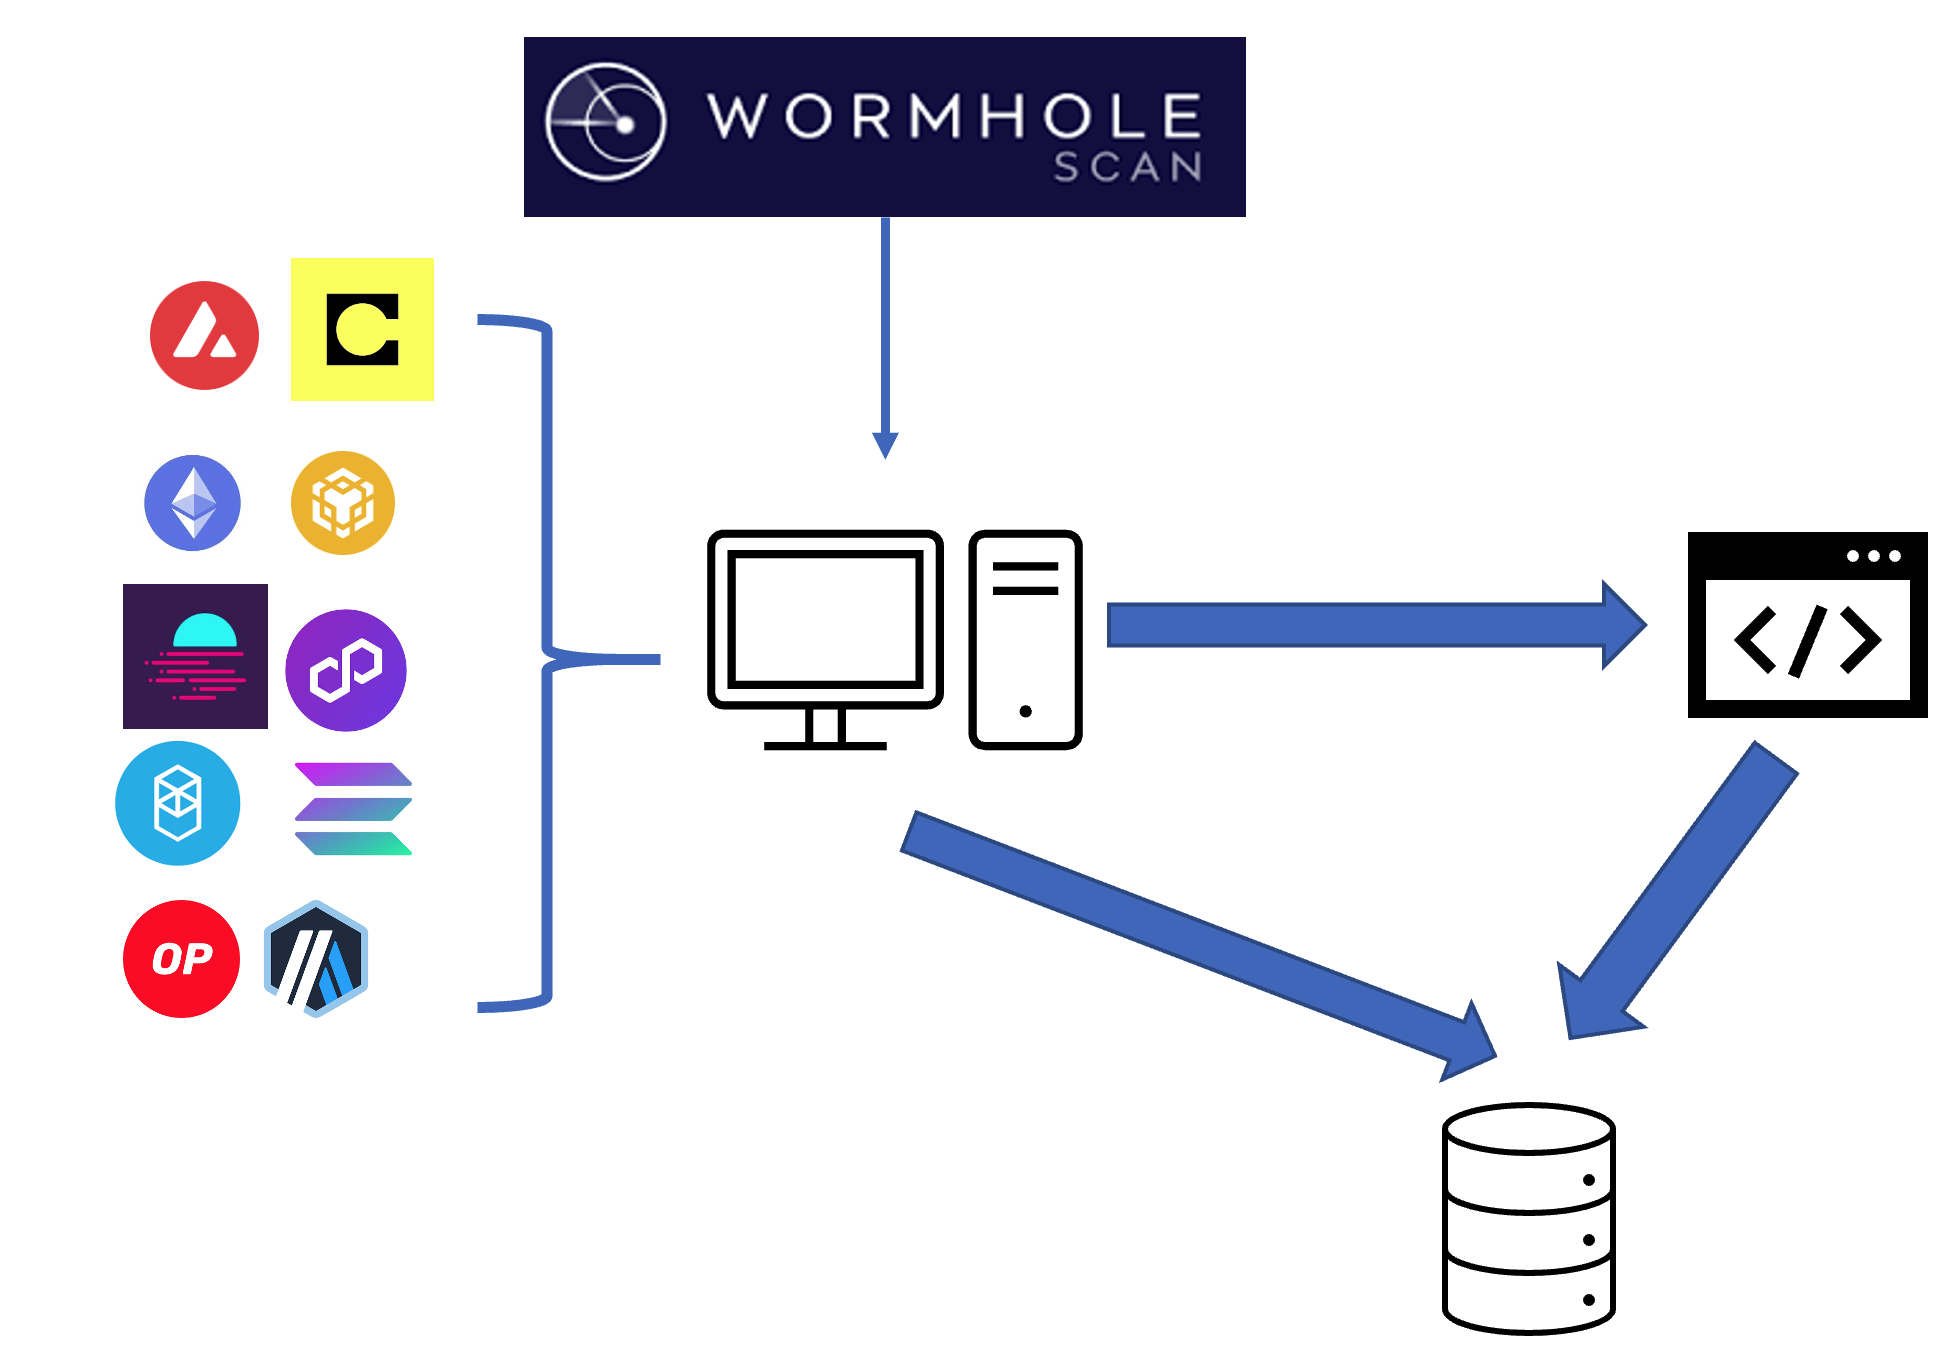
\includegraphics[width=\columnwidth]{fig/dbarch.pdf}
\caption{Live auditing system which consists of three components.}
\label{fig:live-audit-arch}
\end{figure}

%\subsection{Blockchain Monitor}
\textbf{Blockchain Monitor.}
%
The Blockchain Monitor obtains deposit and withdrawal transactions by
periodically retrieving the latest finalized blocks.  The Monitor
% primarily
uses the same commercial RPC services for collecting
Wormhole deposits and withdrawals as we used for the retrospective
analysis (Section~\ref{sec:retro-data}).\footnote{A fully operational
deployment would manage nodes participating in each of the blockchains
to obtain transactions in block data directly.}
%% However, this data
%% is not complete since a withdrawal transaction may reference a deposit
%% on a blockchain not supported by our system or pre-dates our data
%% collection (although infrequent, withdrawals do occur many months
%% after the deposit). To audit withdrawals like these, our system
%% retrieves their corresponding deposit transactions using Wormholescan, a
%% service maintained by Wormhole that indexes bridge
%% transactions. Wormholescan allows us to audit withdrawal transactions
%% whose corresponding deposits are not indexed by our system, improving
%% our audit coverage.\footnote{We note that Wormholescan occasionally
%% returns an error when queried for valid withdrawal transactions, as it
%% focuses on completeness on deposits since users need deposits
%% acknowledged to then trigger withdrawals. We have filed a bug report
%% with Wormhole.}
%% \deian{I would make clear if we actually need Wormholescan to be trustwhorthy or
%% not. I don't think we actually do (but later we bork) so worth clarifying (it
%% only really matters for availability). I would also prefix the Wormholescan
%% bit by saying the RC providers don't let you access ``very old'' events. And I
%% would end this discusison by saying that in practice you would run your own node
%% (which will let you query whatever you want however far back you want).}

% We also note that
The Monitor only retrieves finalized blocks since unfinalized blocks
may be reverted or reordered.  Since different blockchains have
different finality times, we use the timestamp of the latest finalized
block of Ethereum as the synchronization time since Ethereum has the
slowest finality time (around 12 minutes)~\cite{Finality:online}.
%% \footnote{Different systems may have thresholds for
%% finality, but usually wait for at least a few minutes.}
% We leave it to future work to explore how to synchronize to real time.
%% \elisa{It not super clear what the difference between the
%%   synchronization time (15 min) and the refresh time is. So with a
%%   sync time of 15, every time we audit, we are actually 15+10min
%%   behind?}
After retrieving the blocks, the Monitor extracts deposit and
withdrawal transactions for Wormhole and saves them to a local
database.

The polling interval is configurable and the Monitor polls chains
every 1 minute by default.  As a result, the live auditing system is
as recent as the polling interval combined with the finality time
--- a situation similar to bridges due to the polling nature of
distributed off-chain communication.
% We leave it to future work to optimize the delay further.

%% \alex{move wormholescan here.}

%% \geoff{this is the main effort because it needs to be extended for
%%   every chain that we want to audit?  this is where we should say that
%%   we monitor 11 chains (and name at least the popular ones), and
%%   something about why we don't monitor all chains supported by
%%   Wormhole (outside the scope of the approach (Bitcoin), not popular,
%%   etc., can point to previous discussion of which chains are out of
%%   scope.)}

% In addition, for withdraw transactions whose corresponding deposit transactions are on blockchains not supported by our system, we retrieve their corresponding deposit transactions using Wormholescan, a service that scans deposit and withdraw transactions for Wormhole. This setup allows us to audit any withdraw transaction whose corresponding deposit transaction is either on a supported blockchain or is indexed by Wormholescan. Overall, our system can currently audit over 99\% of the withdraw transactions on 11 blockchains, which collectively account for over 95\% of all withdrawal transactions on Wormhole. \alex{our undergrad is adding a blockchain called SUI, which will bump the number to 98\%. im not entire sure if this is necessary}

% The Blockchain Monitor component then extracts deposit and withdrawal transactions from the retrieved blocks. We use commercial RPC services to synchronize with the blockchains. Our system currently supports 11 blockchains, which together account for over 95\% of all withdrawal transactions on Wormhole. \alex{our undergrad is adding a blockchain called SUI, which will bump the number to 98\%. im not entire sure if this is necessary}
%One challenge here is that different blockchains have different finality times. Namely, if a block is not finalized, its transactions may be reverted or reordered. To address this, we always synchronize to the latest finalized block of Ethereum, which is the slowest to reach finality (around 15 minutes). We leave it to future work to explore how to synchronize all blockchains to real time. To bootstrap our database, we preload 2-week of transactions.


% The Blockchain Monitor component synchronizes all 11 blockchains up to a given time and extracts deposit and withdrawal transactions using commercial RPC services. One challenge here is that different blockchains have different finality times. Namely, if a transaction is not finalized, it may be reverted. To address this, we always synchronize to the latest finalized block of Ethereum, which is the slowest to reach finality (around 15 minutes). We leave it to future work to explore how to synchronize all blockchains to real time. To bootstrap our database, we preload 2-week of transactions.
% \alex{key challenge: sync to the same view}

%\subsection{Auditor}
\textbf{Auditor.}
%
For every new withdrawal transaction extracted by the Blockchain
Monitor, the Auditor attempts to find the corresponding deposit
transaction in its local database.  In most cases it will find the
deposit, but if it cannot find it (e.g., because the
withdrawal references a non-existent transaction), the Auditor sends
an email alert inviting manual inspection. If it finds a deposit, it
examines the deposit and withdrawal transactions, and sends an
alert if either the deposit has already been withdrawn (the new
withdrawal is double-spending) or the bridge transaction violates
the balance invariant.



% For every new withdraw transaction extracted by the Blockchain
% Monitor, the Auditor attempts to find the corresponding deposit
% transaction in its local database. If it cannot find the deposit, it

% The Auditor queries the local database to find the deposit transaction.
% In most cases it will find the deposit, but there are several reasons
% why a deposit transaction may not exist in the local database.  

% For
% example, the deposit transaction may pre-date our data collection
% (although infrequent, withdrawals do occur many months after the
% deposit), the deposit transaction may be on a blockchain that is not
% supported by our system, or the withdraw transaction may reference an
% invalid deposit transaction (e.g., Table~\ref{tab:xaction-hashes} in
% the appendix has examples of bridge transactions with invalid deposit
% references). 

%% \geoff{why not just use Wormholescan for everything, is there
%%   something we would miss, or is it a performance/cost optimization?}

%% Using Wormholescan expands our audit coverage to any withdraw
%% transaction whose corresponding deposit transaction is either in the
%% local stored by us locally or is indexed by Wormholescan.\footnote{}

%% Overall, our system can audit over 99\% of the withdraw transactions
%% on 11 blockchains, which collectively account for over 95\% of all
%% withdrawal transactions on Wormhole.

% There are several reasons why a deposit transaction may not exist in our local database. For example, it may be that the deposit transaction is too old and not stored in our database, or the deposit transaction may be on a blockchain that is not supported by our system.

%% For every withdraw transaction, if the deposit transaction is not
%% found, the Auditor component sends an email alert. If a deposit is
%% found, it then checks if the deposit has been withdrawn. If the
%% deposit has been withdrawn, it raises an alert. If the deposit has not
%% been withdrawn, it checks the invariant on the deposit and withdrawal
%% transactions. If the invariant is violated, the Auditor component
%% sends an alert.

% \alex{key challenge: missing data. and the fact that Wormhole has missing data}

%\subsection{Database}
\textbf{Database.}
%
The system uses a PostgreSQL database to store all information
regarding deposit and withdrawal transactions. This information
includes the transaction hash, the blockchain, the amount, and the
timestamp.  It also stores the auditing results, including whether the
deposit has been withdrawn and whether the invariant is
violated.
% \geoff{can be trimmed if we need space}


\subsection{Deployment}
%
We have deployed our live auditing system for the Wormhole bridge for a month.
%% in total starting on \geoff{date}.  \footnote{We report total days
%% because the system is on and off for data available issues and
%% bug-fixes.}
The system audits the deposit and withdrawal transactions between 10
blockchains, which collectively account for around 60\% of all
withdrawal transactions on Wormhole.  For the four weeks that our
system has been operational, it has audited over 60,000 transactions
in total (averaging more than 2,000 transactions per day). The system
currently refreshes every minute (configurable), and sends email
alerts if it observes a transaction violating the balance invariant or
another auditing property (e.g., the destination chain in the deposit
does not match the chain in the withdrawal).

In the time that our system has been operational, it has alerted on 22 transactions in six batches over four weeks. Upon manual inspection, we confirmed that all alerts were caused by previously unseen tokens (recall that in some cases we need to manually account for token-specific logic) or bugs in our code. Consistent with our retrospective analysis, the alert rate is very low at 0.03\% and raises fewer than one alert per day. This rate is on-par with other systems that have an alert budget (e.g., five alerts per day in the context of a lateral movement monitoring system~\cite{ho2021hopper}).
% In the time that we have had the system operational, it has alerted on
% multiple transactions that violated the invariant.  So far these
% transactions have proven to be errors in our implementation (e.g., failed to extract the correct amount) or the RPC services we used (e.g., not indexing a transaction).\alex{add numbers}\alex{add industry numbers}
% When manually inspecting the alerted transactions, we
% discovered that Wormholescan returned incorrect transaction data when
% compared with the transactions stored on-chain (prompting us to notify
% Wormholescan as mentioned above.)

In addition, while we have not observed any attacks during our
monitoring period, we simulated three attack scenarios to confirm that
the system alerts when expected.  These three transactions represent
three types of attacks: (1) a double-spend attack, (2) an
unbacked withdrawal attack, and (3) an attack where the deposit and
withdrawal amounts do not match. The system successfully alerted on
all three. % attacks.

% key: frequency are adjustable


%\section{Improved Architecture\\Incorporating into Bridges\\Protecting Bridges}
\section{Protecting Bridges}
\label{sec:active-protect}

Sections~\ref{sec:retro-results} and~\ref{sec:live-audit} showed how
applying the balance invariant can identify attacks retrospectively and
monitor ongoing transactions as an external third party without any
changes to existing bridge infrastructure.  However, the live
monitoring system only alerts on violations of the invariant and does
not prevent violating bridge transactions from being processed.

In this section, I describe an approach for extending an existing
bridge implementation to prevent malicious transactions from
executing.  Our goal is to present a proof-of-concept implementation
to demonstrate the feasibility of applying the balance invariant in the
workflow of bridge transactions as an active defense against malicious
transactions.  I acknowledge that several practical issues remain
for a complete operational system, presenting an opportunity for
interesting future work.

%% explore the question of whether it is possible to implement a
%% mechanism that stops malicious transactions from execution with
%% minimal code changes.

% how hard it would be to modify the Wormhole bridge to prevent transactions that violate the invariant from being processed. I propose an improved architecture that treats the bridge relaying infrastructure as a black box and can effective stop any malicious transactions that break the invariant and caused by code bugs.

% Below, I start by answering the question of where to introduce the mechanism. Then, using Wormhole as an example, I show how I can modify the bridge to prevent malicious transactions from being processed with fewer than 30 lines of code changes. Finally, I evaluate the security and performance of the improved architecture.

I start by proposing a new model for the workflow of bridge
transactions.  Then, using Wormhole as an example, I show how to
modify an existing bridge implementation to prevent malicious transactions from
being processed with fewer than 30 lines of code changes.  Finally, I
evaluate the correctness and overhead of this initial implementation.

\subsection{The Announce-then-Execute Model}

To guide the design of a new model, I first highlight where the
attack surfaces exist. As shown in Figure~\ref{fig:cross-chain}, a
vulnerability can exist in as early as the second step (verify lock
amount) to as late as the next-to-last step (verify relayed
transaction). Thus, a natural place to introduce a protection
mechanism is just before the final step, which executes the relayed
transaction.

Using this insight I propose an announce-then-execute model.
Figure~\ref{fig:improved-arch} depicts the entities and steps involved
in the new model, focusing on the destination chain (replacing the
right-most box of Figure~\ref{fig:cross-chain}).  The new model
employs two steps to process a withdrawal transaction: (1) verify and
announce the withdrawal transaction on the destination blockchain (steps
8 and 9) and (2) execute the withdrawal transaction (steps 11 and
12). Of particular note, this new model introduces an additional
entity, the \emph{Approver}, which is responsible for approving the
relayed transaction before it is executed.  The Approver can be a bridge
operator, a trusted or trustless third-party (e.g., Bascule~\cite{bascule},
inspired by our work, uses trusted execution environments instead of consensus to ensure the safety of the approver), or a set of
third-parties (e.g., using
multisig for decentralized control). It is responsible for
verifying that the announced withdrawal transaction satisfies the
invariant by validating the same conditions as the Auditor in the live
monitoring system (Section~\ref{sec:live-audit}).  If the relayed
transaction violates the invariant, the Approver can reject the
transaction to prevent it from being executed.

% In addition, I observe that many bridges (e.g., Wormhole) couple the last two steps tightly --- the verification and execution of the relayed transaction are done in the same function call. While being gas efficient, this implementation has a critical drawback. Namely, if the verification function has a bug, it would be impossible to stop the malicious transaction from being executed.

% This means that the verification of a relayed transaction is done at the same time as the execution of the relayed transaction. 

\begin{figure}[t]
\centering
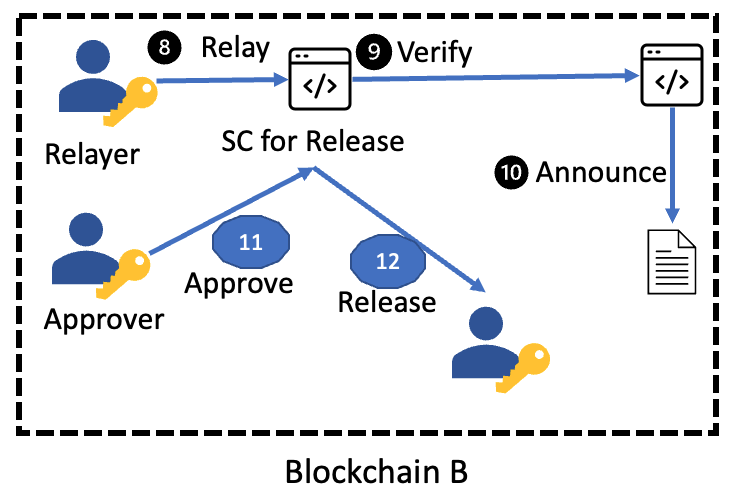
\includegraphics[width=0.9\columnwidth]{fig/improved.pdf}
\caption[Announce-then-Execute Model for Bridges]{Announce-then-execute model for bridges. The approver verifies the relayed transaction before its execution. The approver can be implemented differently (e.g., a set of third-parties), depending on the desired security properties.}
\label{fig:improved-arch}
% \vspace{-0.1in}
\end{figure}


\subsection{Threat Model, Assumptions, and Trade-offs}
I assume that the approver is able to independently verify the relayed transaction and the correct amount of tokens to be transferred. Under this assumption, the announce-then-execute model prevents any implementation bug in any existing bridge components, from step 2 (e.g., the bridge fails to compute the correct deposit amount) to step 8 (e.g., the bridge fails to verify the signature of a relayed transaction). Further, if the 
approver uses secure hardware (namely, HSMs) or a decentralized third-parties
(e.g., with multisig), the model can provide additional protection against
insider threats and key theft (e.g., up to the multisig threshold). Of course,
if the bridge is the only approver, the model does not provide any additional
protection against such insider threats or key theft attacks.


The announce-then-execute model has a few advantages. First, it
explicitly separates the verification and execution of the relayed
transaction, thereby providing an opportunity to reject transactions
that violate the balance invariant.  In comparison, many bridges (e.g.,
Wormhole) couple the last two steps tightly --- the same function call
performs both the verification and execution of the relayed
transaction.  As a result, if the verification step has a bug, it is
not possible to stop violating transactions from being
executed.

Second, the announce-then-execute model allows any external
party, that has visibility into both blockchains, to determine if the
relayed transaction violates the invariant. A long-standing challenge
with bridges is the oracle problem: the destination blockchain does
not have visibility into the source blockchain. The
announce-then-execute model side-steps the oracle problem by allowing
an external party to verify the relayed transaction before it is
executed. This external party can be the bridge operator or a group of third-parties.
Moreover, the announce-then-execute model is compatible with
existing bridges, as it only requires modification to the last step
and treats the relaying infrastructure as well as the verification
code as a black box. In fact, Wormhole's implementation on Solana already separates the process of verifying and executing the relayed transaction, making it even easier to adopt the announce-then-execute model. Had they implemented the announce-then-execute model, the Wormhole bridge would have been able to prevent the \$360M attack on the Solana network~\cite{wormholeattack}.

Lastly, the announce-then-execute model does not
introduce any new attack surfaces --- even if the approver naively
approves all transactions, an attacker still has to exploit other
vulnerabilities in the bridge to profit.

\subsection{Implementation}

%% I took open-sourced Wormhole code written in solidity and modified it to implement the announce-then-execute mechanism.
%% Wormhole's current withdraw function performs two tasks:
%% it verifies the signatures that authorize the withdraw transaction and then executes the withdraw transaction. I split the withdraw function into two separate functions: \texttt{announceWithdraw} and \texttt{approveWithdraw}. The \texttt{announceWithdraw} function handles signature verification and announces the withdraw transaction on the destination blockchain, while the \texttt{approveWithdraw} function executes the withdraw transaction. This modification required fewer than 30 lines of code changes.

Continuing our focus on Wormhole from Section~\ref{sec:live-audit}, I
modified one of Wormhole's open-source contracts to implement the
announce-then-execute model.  Wormhole's current withdrawal function
performs two tasks: it verifies the signatures that authorize the
withdrawal transaction, and then executes it. I
split the withdrawal function into two separate functions:
\texttt{announceWithdraw} and \texttt{approveWithdraw}. The
\texttt{announceWithdraw} function handles signature verification and
announces the withdrawal transaction,
while the \texttt{approveWithdraw} function executes the withdrawal
transaction. This modification required fewer than 30 lines of code
changes.

For simplicity, I opted for a single approver with one key in our implementation. However, our implementation can be easily extended (e.g., to use multisig). In addition, while our implementation has not been adopted by the Wormhole team (as I are a research group not affiliated with Wormhole), our solution has inspired other industry projects to adopt a similar approach~\cite{bascule}.

\subsection{Evaluation}

As a final step I performed a high-level evaluation of the
correctness and overhead (in terms of gas usage) of the
announce-then-execute implementation.  I deployed our bridge
implementation on the Binance and Fantom testnets due to the
availability of free faucets for acquiring testnet tokens for them.
I then executed a series of benign and malicious transactions using
Binance as the source chain and Fantom as the destination chain.

% , and tracked their gas usage during execution.

%% (would be fine if this were a long eval, but since it's so short it's
%% not really needed)
%%
%% I demonstrate that the improved architecture
%% can effectively stop all three malicious transactions while allowing
%% benign transactions to proceed. I also show that the overhead of the
%% improved architecture incurs only a moderate overhead of 50\% more gas
%% usage without any optimization.

\textbf{Correctness.}  For evaluating correctness I disabled the
security checks in the original implementation (e.g., signature
verification) to allow malicious transactions to flow through the
contract implementation (e.g., simulating key compromise).  I then
executed 100 pairs of deposit and withdrawal transactions to validate
that the implementation correctly identifies and protects itself
against malicious transactions that violate the balance invariant.

All but three of the 100 paired transactions were benign, and used
randomly generated values as transaction inputs.
%
The remaining three paired transactions were malicious and were
randomly placed in the transaction sequence.  The malicious
transactions represented the three kinds of bugs underlying the
large attacks in Section~\ref{sec:retro-results}: (1) a bug that
allows a user to withdraw more tokens than they deposited, (2) a bug
that allows a user to withdraw tokens without depositing any
(simulating key compromise), and (3) a bug that allows a user to
withdraw twice from the same deposit (double spending).

The bridge implementation correctly executed the benign transactions
to completion and rejected the three malicious transactions.  The
results are the same independent of where the malicious transactions
randomly appear in the sequence.

\textbf{Overhead.}  The additional steps add overhead to implementing
bridges.  For this experiment, I measured the gas usage for executing
Wormhole's original implementation (with its security checks) and the
gas usage of the announce-then-execute implementation (also with the
original security checks plus our added code).  On average, our
proof-of-concept implementation consumed 110\thou more gas than the
original implementation (370\thou vs.\ 260\thou gas) when
executing the benign transactions, which translates to a
roughly \$1 increase for a typical withdrawal on Ethereum.
% a 50\% increase in gas usage.

I note that our implementation is not optimized for gas usage, and
these results indicate that an
% real
operational deployment
% of the announce-then-execute model
will likely want to reduce the gas overhead of
the additional work (e.g., narrowing to transactions above a threshold
amount of funds).  As discussed further in Section~\ref{sec:discuss},
such optimizations and other practical issues of a real deployment are
interesting future work.




\section{Related Work}
\label{sec:related_work}
There exists a rich literature from both academia and industry that
examines various aspects of spyware apps (e.g., their usage in the
context of intimate partner violence).

Most related to our work, several prior studies have examined
the technical capabilities of spyware apps, including
both industry reports~\cite{PowerPoi79:online, SpyvsSpy59:online,
  ANewWave1:online, Whyyoush17:online, ReverseE12:online,
  YourInfo19:online, Stalking85:online, FlexSpyA1:online,
  diskurse89:online, VB2019Za6:online, SpywareP46:online, Androida91:online} and academic
papers~\cite{parsons2019predator, harkin2019consumer,
  harkin2020commodification, pierazzi2020data,
  feal2020angel,harkin2021operating}. However, many of these
efforts focus on documenting the functionalities supported by the
spyware apps and do not shed light on the implementation used to achieve
different functionalities (mostly because they focus on other facets instead
of the technical implementation challenges). The ones~\cite{Whyyoush17:online,ReverseE12:online,Stalking85:online,FlexSpyA1:online,diskurse89:online,VB2019Za6:online,parsons2019predator} that do study the implementation,
either examined only one or two apps or a small subset of the
mechanisms employed. Our work builds on these studies by systematically and comprehensively analyzing the underlying technical methods that apps employ to acquire different spying capabilities.

Also related, but orthogonal, is work focused on identifying and
detecting spyware apps, both industrial reports listing such
apps~\cite{Tekstalk86:online, esetandr4:online, ch33r10S37:online} and
academic efforts to characterize and build detection algorithms for
them~\cite{almansoori2022global,pierazzi2020data, chatterjee2018spyware, han2021towards,
  saroiu2004measurement, egele2007dynamic, roundy2020many,
  wang2006netspy, moshchuk2006crawler, randall2020trufflehunter}.  Yet
another related body of work examines spyware apps' presence in
different contexts such as intimate partner violence and
cyberstalking~\cite{havron2019clinical,freed2019my,tseng2020tools,thomas2021sok,freed2018stalker,fraser2010new,
  shimizu2013domestic,woodlock2017abuse,southworth2005high,southworth2006technology,dragiewicz2019domestic,mayrhofer2021android,motherboardstalkerwaremarket}.
I believe our findings, particularly characterizing the data access
mechanisms used by spyware, will be of use to those implementing
detectors, but detection is not itself a goal of our work.


Outside the context of spyware, another related research
domain has focused on how various kinds of malware (including spyware)
can abuse Android APIs to achieve abusive functionality.  In
particular, several papers have also identified abuse of the Android
Accessibility APIs, starting with Kraunelis et
al.~\cite{kraunelis2013malware}.  Following this line of work,
Fratantonio et al.~\cite{fratantonio2017cloak}, Kalysch et
al.~\cite{kalysch2018android}, Diao et al.~\cite{diao2019kindness},
and Naseri et al.~\cite{naseri2019accessileaks} have documented how
Accessibility can be abused in various contexts.  While several of
these papers suggest potential fixes, Huang et
al.~\cite{huang2021a11y} is the first to describe a comprehensive
framework for mitigating misuse in the accessibility API.  Others have
explored other forms of API abuse, including Audio and Video
APIs~\cite{petracca2015audroid, pan2018panoptispy}, screenshot API~\cite{sbai2022threat}, device
administration APIs~\cite{shan2019device}, WebView-related APIs~\cite{luo2011attacks, chin2013bifocals, neugschwandtner2013view, ZhangIdentity2022}, the use of overlays in
malware~\cite{yan2019understanding}, and mechanisms for app
hiding, discovery~\cite{shan2018self, pham2019hidemyapp} and
persistence~\cite{zhou2020demystifying}.  Our work builds on all of
these efforts, but rather than exploring these issues abstractly,
focuses specifically on how they manifest in consumer mobile spyware
in the wild.  Our detailed analysis not only confirmed that the consumer spyware sector exploits similar techniques documented in broader mobile malware, but also uncovered two new forms of API
abuse (invisible camera access and hiding app icons) that appears to have originated from within the spyware ecosystem.

Finally, spyware companies have a long history of poor security hygiene.
% There have been
Numerous media reports describe data breaches at various spyware companies, including Spyhuman~\cite{HackerSt66:online}, TheTruthSpy~\cite{Companyt8:online}, mSPY~\cite{mSpybrea38:online,mSpyCybe86:online}, Cerberus~\cite{Cerberus12:online}, Flexispy~\cite{Stalkerw59:online}, Mobistealth~\cite{HackerSt50:online}, Spyfone~\cite{Spywaref13:online}, Retina-X~\cite{RetinaXa98:online, Hackercl62:online}, among others. These breaches have exposed hundreds of thousands (if not millions) of users' sensitive personal information (e.g., location, videos, etc.) to the broad public. Our work is responsive to these events and seeks to explore the nature of the security protections provided by spyware vendors and the extent to which these breaches have led to improved practices. While recent, contemporaneous report from ESET~\cite{esetandr4:online} also investigated similar issues, our work is distinct in analyzing the security of each app from the context of protecting user data and presents a detailed, documented, and reproducible methodology.

% others have also investigated privacy deficiencies of Android apps, they either focus on one particular issue~\cite{santhanam2022scraping} or lack a detailed, documented, and reproducible methodology~\cite{esetandr4:online}.

% \footnote{Contemporaneously with our research, a recent report from ESET~\cite{esetandr4:online} also documents a range of Android spyware service vulnerabilities.  Our work is similarly motivated but is distinct in analyzing the security of each from the context of protecting user data.}


%While the research community has not examined the security of spyware apps to best of our knowledge, there is a large body work on the security of apps in other contexts, including those that study the (in)security of financial apps~\cite{reaves2017mo,yang2017show, kaur2018security, chen2018mobile,kim2017breaking, chothia2017banker}, TLS and SSL (in)security~\cite{oltrogge2021eve, fahl2012eve, greenwood2014smv, possemato2020towards, onwuzurike2015danger}, and misuse of cryptographic libraries~\cite{egele2013empirical}. \alex{how do I differentiate ourselves?}.


%\section{Limitations}
While our approach captures a variety of vulnerabilities, it is by no means exhaustive. For example, a key assumption we make is that withdrawal are done through designated withdraw functions. However, if an adversary is able to compromise the key to account that holds the funds for the bridge, they could simply transfer the funds to another account and then withdraw them without going through the designated withdraw function(s). Similarly, if an adversary is able to withdraw funds by repurposing other functions (e.g., the deposit function), our approach would not detect it. Moreover, if an attack transaction does not involve a withdrawal, our approach would not detect it. Last but not least, if an attack is somehow able to profit without breaking the balance invariant, our approach would not detect it.  However, we believe that our approach is a important first step in using accounting principles to protect bridges from theft and that it can be extended to address these and other vulnerabilities in the future.

\section{Ethics}
\label{sec:ethics}

We believe our work, which deals with public data, no identified
individuals and a simple means for identifying attacks on crypto token
transfer bridges (and potentially preventing such attacks in the
future), has very low ethical risk and significant upside. Moreover, I have attempted to disclose significant suspicious bridge
transactions to appropriate bridge operators (yet with limited
success as most of the bridges have ceased operations). Lastly, I will make our code and data available upon publication.
% 
% We strictly use public data and to
% the extent that I identify outcomes (e.g., attacks) they are at the
% granularity of bridges and blockchains, not individuals.

% As well,


% Considering the Menlo report principle of ``Respect for Persons'', we
% are not dealing with, nor do I attempt to analyze, data at the
% granularity of individual persons.  We strictly use public data and to
% the extent that I identify outcomes (e.g., attacks) they are at the
% granularity of bridges and blockchains, not individuals.  Similarly,
% with respect to the principle of ``Justice'', I have no reason to
% believe that our analysis discriminates at the level of persons or
% distinct groups of persons --- all users of bridges should benefit
% equally (excepting criminals).  On the topic of ``Respect for Law and
% Public Interest'', I are engaging with existing public data, I have
% documented our methods clearly and I are careful to limit our factual
% statements to those for which I have evidence.  As well, I have made
% a point to disclose significant suspicious bridge transactions to appropriate
% bridge operators.


% We believe our work, which deals with public data, no identified
% individuals and a simple means for identifying attacks on crypto token
% transfer bridges (and potentially preventing such attacks in the
% future), has very low ethical risk and significant upside.  However,
% in the interest of due diligence, I provide a more thorough
% justification of this position following the Menlo Report principles
% as indicated by the USENIX Security call.

% Considering the Menlo report principle of ``Respect for Persons'', we
% are not dealing with, nor do I attempt to analyze, data at the
% granularity of individual persons.  We strictly use public data and to
% the extent that I identify outcomes (e.g., attacks) they are at the
% granularity of bridges and blockchains, not individuals.  Similarly,
% with respect to the principle of ``Justice'', I have no reason to
% believe that our analysis discriminates at the level of persons or
% distinct groups of persons --- all users of bridges should benefit
% equally (excepting criminals).  On the topic of ``Respect for Law and
% Public Interest'', I are engaging with existing public data, I have
% documented our methods clearly and I are careful to limit our factual
% statements to those for which I have evidence.  As well, I have made
% a point to disclose significant suspicious bridge transactions to appropriate
% bridge operators.

% Finally, on the topic of ``Beneficence'', we
% identify the three sets of stakeholders in our work.  These include
% the past and (potential) future victims whose investments, both direct
% and indirect, via token transfer bridges have been undermined by
% large-scale thefts from these services.  In addition, other
% stakeholders include bridge operators and, finally, the criminal actors who
% derive income from vulnerabilities in bridges.  We argue that our
% retrospective analysis creates no direct new harm for any parties ---
% these attacks have already happened.  For bridge operators, our
% analysis may create some potential liability in supporting a civil
% claim of poor stewardship, but at the same time our documentation of
% the widespread nature of this problem provides a ``common practice''
% defense.  Some of the unilateral transfers I have documented, if they
% were illegitimate (which I do not know), could also create liability
% for bridge operators, but I believe this potential harm is balanced
% against the interest of investors in transparency and fairness in
% operating financial services.  Finally, for our proposed real-time
% analysis approaches, if these were adopted by bridge operators, it
% could foreclose a broad range of attacks.  We admit that this outcome
% could harm our criminal stakeholders as it might deny them of an
% important income stream.  Knock on effects could include a reduction
% in revenues for online crypto money laundering services and Lamborghini
% dealerships, but I believe this is well-justified by the concordant
% reduction in victimization.





\section{Conclusion}
Consumer mobile spyware persists because it exists in a gray area: not
clearly legal, but not canonically illegal; not allowed in the app
store, but broadly available via side loading; not supported by APIs
but able to achieve its ends through manipulation and trickery;
repeatedly breached, but able to maintain market power because those
injured are not its customers.

For example, the use of such software to monitor arbitrary individuals
without consent is clearly illegal --- both due to violations of the
Computer Fraud and Abuse Act (18 USC 1030) and provisions of the
Wiretap Act (18 USC 2511).  However, contemporary mobile spyware
companies argue that they do not support or encourage such uses.
Indeed, since the Department of Justice brought a criminal indictment
against the makers of StealthGenie~\cite{dojstealthgenie} in 2014,
spyware vendors have generally restricted their public marketing to
focus on the monitoring of minor children (whose consent is abdicated
to their guardians) or the monitoring of employees (such monitoring
can be viewed as consensual when the equipment is owned by the
employer and employees are clearly informed about the policies around
monitoring).  However, this shift in ``official'' marketing has done
little to undermine the large market for using this software illegally
and a broad array of sites and forums provide detailed direction on
how to use such apps to covertly monitor a spouse or partner.

Similarly, while curated app stores, such as Google Play Store, now
disallow such apps from being sold, Android's default support for
sideloading makes this limitation only a minor obstacle for someone
seeking to surreptitiously install spyware on a
%target
phone.

Moreover, the fact that spyware abusers are able to obtain physical
access to a device (at least temporarily), renders Android's
finer-grained permissions checks ineffectual as well.  The one-time
``consent'' provided by the spyware installer provides largely
unfettered capabilities that the true user may never be aware of.  The
Accessibility API offers a particularly large consent loophole, as its
intended function necessitates almost complete mediation of I/O
activities.  Moreover, even when the API itself has been changed to
restrict certain capabilities I have repeatedly found spyware authors
creatively abusing APIs or their implementations to gain capabilities
that were not meant to be available to third-party apps
(e.g., the range of mechanisms described in
Section~\ref{subsubsec:audio_recording} for covertly performing audio
recording in spite of multiple OS changes intended to prevent such
abilities). I uncover Android's incomplete threat model
with our discovery of their unwillingness to fix what
I consider to be a vulnerability in their API that allows spyware apps to
hide their icon.

The privacy deficiencies I uncover in Section~\ref{sec:data-leak}, on
the other hand, demonstrated the unfortunate truth about consumer
mobile spyware apps: that they prioritize covert collection over
protecting user data.  As an example, Spapp shows signs of
significant developer effort: it implements most of the technical
collection capabilities I have described and carefully obfuscates its
code to hinder reverse engineering efforts. However, the same app
places little investment in protecting the data it has collected,
incorrectly handling data retention after deletion and executing
highly sensitive SMS commands without authentication.  Sadly, this
situation is far from the exception --- and the range of past data
breaches are testament to this asymmetry.  Moreover, because it is
victims who suffer here and not spyware customers, there are no market
forces that will correct this state of affairs.

All of these challenges highlight the need for a more creative,
diverse and comprehensive set of interventions from industry,
government and the research community.  While technical defenses can
be part of the solution (and particularly OS improvements that make
users aware of their \emph{current} exposure, like the new privacy
dashboard in Android 12), consumer spyware's persistence and growth
suggests that a broader range of measures including payment
interventions~\cite{mccoy2012priceless}, regulatory crackdowns (e.g., FTC
recently banned SpyFone from operating~\cite{FTCFinal26:online}) and
further law enforcement action may also be necessary to prevent
surveillance from becoming a consumer commodity.


Chapter~\ref{chap:pets23}, in part, is a reprint of the material as it appears in Proceedings on Privacy Enhancing Technologies 2023. Enze Liu, Sumanth Rao, Sam Havron, Grant Ho, Stefan Savage, Geoffrey M. Voelker, and
Damon McCoy. The dissertation author was the primary investigator and author of this paper.


%In this work, I perform an in-depth technical analysis of fifteen consumer spyware apps targeting Android phones. I document how spyware apps abuse of Android APIs to achieve a wide range of capabilities --- ranging from surreptitiously collecting users data to persisting on the target device. Our technical analysis not only sharpens the understanding of consumer mobile spyware, but also sheds light on the challenges of defending against spyware apps and the need for more creative defense mechanisms from both Google and the research community.

%Defending against spyware apps is challenging due to the unique threat model they pose. First, the adversary has physical access and perform various actions such as granting permissions. Many existing defense mechanisms appear unsuccessful against spyware apps as they assume the user is benign and will grant permissions consciously.
%For instance, Android~10 limited when apps can start Activities to a few scenarios~\cite{Restrict50:online}
%(e.g., if an app is an accessibility service or has acquired the \texttt{SYSTEM\_ALERT\_WINDOW} permission).
%While this restriction should hinder any abuse that relies on Activities, it is insufficient against spyware apps because the apps can register themselves an accessibility service and request \texttt{SYSTEM\_ALERT\_WINDOW} permission,
%which the stalker (abuser) can grant upon installation given their physical device access.
%This also applies to several academic papers~\cite{huang2021a11y,pan2018panoptispy} that assume the user is benign.
%Next, the fact that many spyware apps are sideloaded renders defense systems that are deployed on app markets (e.g., Google Play Policies and Yan et al.~\cite{yan2019understanding}) unusable. Furthermore, while the apps that I study are dedicated for spying on users, past literature~\cite{chatterjee2018spyware,havron2019clinical,roundy2020many} has shown that benign apps that can be repurposed for spying, which further blurs the lines between benign and malicious apps. Lastly, there exists a natural tension between some functionalities (e.g., accessibility) and enabling spyware. As I have shown, while the introduction of some accessibility APIs (e.g., taking screenshots and audio recording) certain benefits the disabled users, it also makes it easy for spyware apps to perform certain actions.






%In summary, I perform the first technical analysis of fifteen Android spyware apps targeting as well as
%document the measures taken by
%each app to protect the privacy of the sensitive data they collect. I work not only sheds light on the technical capabilities and insecurity of spyware apps but also provides guidance both for phone OS vendors and regulators in their efforts to undermine the use and availability of such software.

%\alex{other text that might be useful}

%======== Random Text ========


%Our in-depth technical analysis of fifteen apps reveals three noticeable themes:
%(1) the arms race between spyware authors and defenses employed by Android; and
%(2) the two classes of spyware apps (those that are innovative and those that use standard techniques).

%First, the arms race between spyware authors and defenses employed by Android is clear over the course of our analysis:
%Android keeps patching known exploits while spyware authors constantly seek for new ways to abuse the system.
%For example, as described in Section~\ref{subsubsec:audio_recording}, spyware apps have adapted their ways to covertly perform audio recording to circumvent the protections Android introduced in multiple patches (e.g., protecting {VOICE\_CALL} with a permission in Android~6 and filtering unsolicited calls to set \texttt{AudioSource} in Android~9).
%\grant{There's something off with the grammar in ``to set \texttt{AudioSource}'', and I'm not sure what we're trying to say.}
%Similarly, with respect to screenshots, Android~10 restricted the ability to take screenshots via \texttt{MediaProjection};
%in response, several spyware apps evolved by abusing the takeScreenshot API of AccessibilityService introduced in Android~11.

%Next, I observe two classes of spyware apps: those that are innovative and drive the evolution of spying techniques, and those that use standard techniques. For example, \textsc{spy24} has two novel ways of abusing the Android system that are not observed in any other apps (using an invisible browser to stream videos and exploiting TV app features to hide its icons).
%Notably, \textsc{spy24} can successful hide its icon even in the latest Android~12.

% Given the amount of sensitive user data these apps collects, one would expect more safeguards to have been in place to better protect user data.

%\section{Conclusion}

% \section{The Invariant}
\alex{Describe the invariant here (using source and dst).}
We observe that for token transfer bridges—those that facilitate the transfer of tokens between blockchains without performing token swaps—the inflow and outflow of tokens should be equivalent after factoring in fees. In other words, the outflow should be strictly less than or equal to the inflow due to the presence of fees. I refer to this principle as the invariant.


Below, I describe how the various attacks violate the invariant. For buggy deposit verification, an attacker deposits less than the amount withdrawn, resulting in a scenario where outflow exceeds inflow. For buggy event verification, compromised relaying key and compromised submitter key, the attacker withdraws assets that were never deposited, resulting in a scenario where inflow is zero and outflow is non-zero. For buggy withdraw verification, if the attacker can verify arbitrary payload, then the inflow is zero and outflow is non-zero. If the attacker can replay a message, then the inflow is non-zero and outflow is greater than inflow. In summary, in all cases, the invariant is in that the outflow is strictly greater than the inflow, rather than equal to or less than the inflow.

\alex{has been done at a grand scale}

\alex{add a figure to illustrate the invariant.}

% \clearpage


\section*{Open Science Policy}

I will make all of our data, results, and code public upon
publication. In addition, I have already included some of the most
important results in the appendix.

\section{Ethics}
\label{sec:ethics}

We believe our work, which deals with public data, no identified
individuals and a simple means for identifying attacks on crypto token
transfer bridges (and potentially preventing such attacks in the
future), has very low ethical risk and significant upside. Moreover, I have attempted to disclose significant suspicious bridge
transactions to appropriate bridge operators (yet with limited
success as most of the bridges have ceased operations). Lastly, I will make our code and data available upon publication.
% 
% We strictly use public data and to
% the extent that I identify outcomes (e.g., attacks) they are at the
% granularity of bridges and blockchains, not individuals.

% As well,


% Considering the Menlo report principle of ``Respect for Persons'', we
% are not dealing with, nor do I attempt to analyze, data at the
% granularity of individual persons.  We strictly use public data and to
% the extent that I identify outcomes (e.g., attacks) they are at the
% granularity of bridges and blockchains, not individuals.  Similarly,
% with respect to the principle of ``Justice'', I have no reason to
% believe that our analysis discriminates at the level of persons or
% distinct groups of persons --- all users of bridges should benefit
% equally (excepting criminals).  On the topic of ``Respect for Law and
% Public Interest'', I are engaging with existing public data, I have
% documented our methods clearly and I are careful to limit our factual
% statements to those for which I have evidence.  As well, I have made
% a point to disclose significant suspicious bridge transactions to appropriate
% bridge operators.


% We believe our work, which deals with public data, no identified
% individuals and a simple means for identifying attacks on crypto token
% transfer bridges (and potentially preventing such attacks in the
% future), has very low ethical risk and significant upside.  However,
% in the interest of due diligence, I provide a more thorough
% justification of this position following the Menlo Report principles
% as indicated by the USENIX Security call.

% Considering the Menlo report principle of ``Respect for Persons'', we
% are not dealing with, nor do I attempt to analyze, data at the
% granularity of individual persons.  We strictly use public data and to
% the extent that I identify outcomes (e.g., attacks) they are at the
% granularity of bridges and blockchains, not individuals.  Similarly,
% with respect to the principle of ``Justice'', I have no reason to
% believe that our analysis discriminates at the level of persons or
% distinct groups of persons --- all users of bridges should benefit
% equally (excepting criminals).  On the topic of ``Respect for Law and
% Public Interest'', I are engaging with existing public data, I have
% documented our methods clearly and I are careful to limit our factual
% statements to those for which I have evidence.  As well, I have made
% a point to disclose significant suspicious bridge transactions to appropriate
% bridge operators.

% Finally, on the topic of ``Beneficence'', we
% identify the three sets of stakeholders in our work.  These include
% the past and (potential) future victims whose investments, both direct
% and indirect, via token transfer bridges have been undermined by
% large-scale thefts from these services.  In addition, other
% stakeholders include bridge operators and, finally, the criminal actors who
% derive income from vulnerabilities in bridges.  We argue that our
% retrospective analysis creates no direct new harm for any parties ---
% these attacks have already happened.  For bridge operators, our
% analysis may create some potential liability in supporting a civil
% claim of poor stewardship, but at the same time our documentation of
% the widespread nature of this problem provides a ``common practice''
% defense.  Some of the unilateral transfers I have documented, if they
% were illegitimate (which I do not know), could also create liability
% for bridge operators, but I believe this potential harm is balanced
% against the interest of investors in transparency and fairness in
% operating financial services.  Finally, for our proposed real-time
% analysis approaches, if these were adopted by bridge operators, it
% could foreclose a broad range of attacks.  We admit that this outcome
% could harm our criminal stakeholders as it might deny them of an
% important income stream.  Knock on effects could include a reduction
% in revenues for online crypto money laundering services and Lamborghini
% dealerships, but I believe this is well-justified by the concordant
% reduction in victimization.





% \section{Approach}
\label{sec:meth}

The core hypothesis of our work is that value should be conserved
within cross-chain transactions.  That is, that the value of the asset
inflow in such a transaction (i.e., the deposit) should equal the
value of the asset outflow (i.e., the withdrawal).  In token transfer
bridges, this invariant corresponds to a balancing of the inflow
tokens and the outflow tokens (less any fees or transaction costs
incurred by the bridge itself).  When this balance invariant does not
hold it allows a range of opportunities for fraud, all of which
involve greater outflows (withdrawals) than inflow
(deposits). Figure~\ref{fig:invariant} illustrates such an outcome by 
graphing the \emph{aggregate} difference between bridge inflow (on
Ethereum) and outflow (on Solana) leading up to and during the
February 2022 attack on the Wormhole bridge.  The net difference is
consistently near zero, with only short positive deviations
(representing delayed withdrawals) until the attack in January, at
which point there are significant withdrawals without matching
deposits---producing a large negative difference.

Testing this invariant on a \emph{per transaction basis} is
straightforward in principle. However, since bridge transaction formats are
not standardized, it requires a range of per-bridge and per-chain
parsing in practice.  Our methodology for normalizing this information
focuses on two key pieces of information: a) identifying each bridge
transaction---a composite of a deposit (inflow) transaction on a
source blockchain and a withdrawal (outflow) transaction on
another---and b) identifying the value transferred in each such bridge
transaction.

\begin{figure}[t]
  \centering
  \includegraphics[width=0.7\columnwidth]{fig/sec25_plot_wormhole.pdf}
  \caption{Total Inflow (on Ethereum) - Total Outflow (on Solana) Over Time: Wormhole Attack in Feb 2022.}
  \label{fig:invariant}

\end{figure}


\subsection{Identifying Bridge Transactions}
For almost all bridges, identifying their component (per-chain) inflow
and outflow transactions is straightforward --- bridges typically use
explicit events on each chain to signal if a given transaction is a
deposit or withdrawal.\footnote{One key exception to this rule is the
  Wormhole bridge which, until late 2023, did not emit specific
  events when executing a withdrawal transaction.  In this case, we infer that a withdrawal took
  place by looking for transactions that invoke functions designated for performing withdrawal operations (e.g., \textit{completeTransfer}).
  %have synthesized such an event ourselves by parsing the function
  % names called by the transaction to .  
  It also appears to be widely understood today that emitting
  explicit events is a best practice.}

Pairing these component transactions (i.e., matching deposits on one
chain to withdrawals on other) can be performed in several different
ways.  The easiest, and most common, is via a unique transaction
identifier. Such IDs are typically generated by the bridge on the
\emph{source chain} during a deposit transaction and then copied into
the withdrawal transaction on the destination chain.\footnote{These
  unique IDs are commonly simple global variables incremented with
  each new transaction.}  However, instead of an explicit ID, some
bridges use a hash of the deposit transaction for the same purpose
(e.g., for Anyswap, each withdraw transaction will include the hash of
its corresponding deposit transaction).\footnote{We note that to prevent potential replay attacks, bridge implementers should also include an ID that uniquely identifies individual deposit events within a transactions. Sadly, this is often not the case.}  Finally, in a handful of cases there are
no ``inband'' identifiers that can be used to associate transactions.
We believe this is a poor design choice that is fundamentally in
conflict with auditability.  However, even in these cases, for the
purpose of our analysis we have been able to pair transactions using
explicit query APIs provided by the affected bridges
services.\footnote{For example, when a bridge transaction on the Poly
  Network bridge includes a withdrawal from Curve (a kind of liquidity
  pool) or when a bridge transaction on the Binance Token Hub includes
  a Binance Smart Chain (BSC) withdrawal, it is not possible to
  identify the partner deposit from blockchain data alone and we must
  make use of ``out of band'' data available through their respective
  bridge query APIs.}

  At the end of this process, we identify a comprehensive collection
  of ``bridge transactions'' (a pair of transactions from two
  different blockchains that were used by the bridge to transfer
  value across them). While the vast majority of bridge transactions
  are pairs of deposit and withdrawal transactions, a handful of
  bridge transactions are either withdrawal-only (e.g., in the case of
  attacks) or deposit-only (e.g., if the user chooses to delay their
  withdrawal).

% And for 
% a handful of bridge transaction, they are either withdrawal-only or deposit-only, and we treat them as singleton transactions.
%  and a handful of singleton
% transactions (i.e., which involve the bridge, based on their
% addresses, but are withdrawal-only or deposit-only).


%For example, with the Binance bridge, the matching transaction for a BSC transaction can only be identified by querying the API. 
%%% here.
%Similarly, for Poly Network bridge, when users withdraw from Curve (a kind of liquidity pool), the matching deposit amount is not recorded on the blockchain, as its a special type of withdrawal where the matching deposit is computed off-chain and only available through the API. In this case, we also rely on Poly Network's API to pair the deposit and withdraw transactions, if the deposit transaction is from Curve. \elisa{It might be nice to give a reason why the pairing info is not available for these cases if we know.} 




%\textbf{Using Unique ID.} Most of the bridges\alex{how many?} will create a unique id for each deposit transaction (incrementing by 1).
%A withdraw transaction will contain this unique id. We can then use this unique id to pair the deposit and withdraw transactions.



%\textbf{Using the transaction hash of the deposit transaction.}
%Another way to pair deposit and withdraw transactions is to use the transaction hash of the deposit transaction. A withdraw transaction will include the transaction hash of the corresponding deposit transaction hash. We can then use this information to pair the deposit and withdraw transactions.

%\textbf{Using the official API.}
%Some bridges provide APIs to query matching deposit and withdraw transactions. While this feature mostly exist for user convenience, sometimes we have to rely on this API to pair deposit and withdraw transactions, as the pairing information is not directly available as part of the withdraw transaction.\alex{maybe we should hedge here and say its not trivial to get the information.} 
%For example, with the Binance bridge, the matching transaction for a BSC transaction can only be identified by querying the API. 
%%% here.
%Similarly, for Poly Network bridge, when users withdraw from Curve (a kind of liquidity pool), the matching deposit amount is not recorded on the blockchain, as its a special type of withdrawal where the matching deposit is computed off-chain and only available through the API. In this case, we also rely on Poly Network's API to pair the deposit and withdraw transactions, if the deposit transaction is from Curve. \elisa{It might be nice to give a reason why the pairing info is not available for these cases if we know.} 

\subsection{Identifying the Value Transferred}
Many bridge transaction event formats explicitly identify the amount
and kind of tokens transferred. However, some bridges do not emit this
information and others can be unreliable.\footnote{For example, as
  mentioned earlier, pre-2024 Wormhole does not emit an event for
  withdrawal transactions. Other examples include the Meter bridge and
  Qubit bridge, which attempted to verify the number of tokens
  received but had exploitable bugs.}  In such cases, we can
frequently make use of the ERC-20 ``Transfer'' event (see
Figure~\ref{fig:erc20-event} for an example) that is emitted when the
contract transfers the tokens from the user's account to the bridge's
account.  This event contains the number of tokens transferred as well
as the sender and recipient addresses, which we use to identify the
number of tokens transferred to or from the bridge.  Because the
Transfer event is adjacent to its associated bridge-generated event,
it is easy to identify and thus establish the number of tokens
transferred.\footnote{As a sanity check, we also require that the
  sender and recipient addresses in the Transfer event are consistent
  with the bridge's defined behavior: for withdrawal transactions, we
  require that the sender is either a mint address (i.e., all-zero
  address) or a bridge-controlled address, while for deposit
  transactions, we require that the recipient is either a burn address
  (i.e., all-zero address) or a bridge-controlled address.}  In a few
implementations, multiple related Transfer events can be emitted at
once, and in these cases we have manually inspected their contracts
and constructed implementation-specific logic to account for this
behavior.  Another special case is caused by so-called ``reflection
tokens'' in which the number of tokens logged in the event (the value
field in Figure~\ref{fig:erc20-event}) is dynamically adjusted based
on a combination of the intended number and the total token supply.
For such cases, we either rely on bridge events which capture the
intended number of tokens transferred or implement token-specific
logic to recompute the value accordingly.  Finally, native tokens have
no Transfer event (since they are not ERC-20 tokens), but thus far we
have either been able to recover the number of tokens transferred from
bridge events or so-called ``internal transactions''.

To summarize, while it is certainly possible to create a bridge
transaction protocol that records insufficient data to match deposits
and withdrawals, or for which the number of tokens transferred might
be ambiguous, our empirical experience analyzing 11 bridges and 21
blockchains is that such reconstruction has always been possible.


%When the amount of tokens transferred logged by the bridge is unavailable or unreliable, we can use the Transfer event emitted by an ERC20 token contract to identify the amount of tokens transferred. The Transfer event, part of the ERC20 standard, has been used by prior research in other scenarios.\alex{cite} This event contains the amount of tokens transferred as well as the sender and recipient addresses, which we use to identify the amount of tokens transferred to or from the bridge. Concretely, we observe that for any successful bridge transaction, depending on the order of execution, the transfer event either happens right before or after the bridge-generated event. As a result, we can first locate the bridge event and then look for the Transfer event that happens right before or after the bridge event, which contains the amount of tokens transferred. As additional sanity checks, we also require that the sender and recipient addresses in the Transfer event are consistent with the bridge's behavior. Namely, for withdraw transactions, we require that the sender is either a mint address (e.g., all-zero address) or a bridge controlled address. On the other hand, for deposit transactions, we require that the recipient is either a burn address (e.g., all-zero address) or a bridge controlled address.\alex{do we have to explain the intuition?}


%There are two ways to identify the amount of tokens transferred by the bridge: using the amount logged in a 
%bridge-generated event or using the Transfer event emitted by ERC20 tokens. Specifically, some bridges include the amount of tokens sent or received in their events. However, this information is not always reliable, as bridges can have bugs (typically when they don't verify the amount of tokens they actually received), which is the case for [AL: which]. Additionally, some bridges do not emit this information. In such cases, we can use the token transfer event to identify the amount of tokens transferred, which also serves as the ground truth.

%\textbf{Identifying Token Transferred from Transfer Event.} 
%When the amount of tokens transferred logged by the bridge is unavailable or unreliable, we can use the Transfer event emitted by an ERC20 token contract to identify the amount of tokens transferred. The Transfer event, part of the ERC20 standard, has been used by prior research in other scenarios.\alex{cite} This event contains the amount of tokens transferred as well as the sender and recipient addresses, which we use to identify the amount of tokens transferred to or from the bridge. Concretely, we observe that for any successful bridge transaction, depending on the order of execution, the transfer event either happens right before or after the bridge-generated event. As a result, we can first locate the bridge event and then look for the Transfer event that happens right before or after the bridge event, which contains the amount of tokens transferred. As additional sanity checks, we also require that the sender and recipient addresses in the Transfer event are consistent with the bridge's behavior. Namely, for withdraw transactions, we require that the sender is either a mint address (e.g., all-zero address) or a bridge controlled address. On the other hand, for deposit transactions, we require that the recipient is either a burn address (e.g., all-zero address) or a bridge controlled address.\alex{do we have to explain the intuition?}

%\textbf{Additional Considerations.}
%We note a few additional considerations. First, while the transfer action usually results in a single event, there are cases where multiple Transfer events are emitted. In such cases, we need to incorporate token-specific logic to capture a series of Transfer events to identify the amount of tokens transferred. For tokens exhibiting this behavior, we manually examine their code and account for their logic in our analysis.
%Next, for transfers involving native tokens, the value sometimes is included in internal transactions, and no event is emitted. We use the internal transactions to identify the amount of tokens transferred. Lastly, for a special type of tokens called reflection tokens, we need to account for the reflection mechanism. Specifically, reflection tokens have a mechanism where the real amount of tokens transferred is dynamically adjusted based on intended amount and total supply. For some tokens, they emit events that include enough information to recompute the intended amount. We thus use this information to identify the intended amount of tokens transferred. For other tokens, they do not provide such information. However, for those cases, conveniently, the bridge event includes the intended amount of tokens transferred. We thus revert back to use the amount logged by the bridge.\footnote{The delta between the intended amount and the real amount is very small (typically within a factor of 0.01). Thus, even if the initial amount is not logged by the bridge, the intended amount can still be bounded.}

\subsection{Checking the Balance Invariant}
Once we have identified both sides of the bridge transaction and the
number of tokens transferred by the bridge, we can verify if the
balance invariant holds: for each bridge transaction (including those
that are withdrawal-only), does the number of tokens transferred from
the bridge---the withdrawal amount---match the number of tokens
received by the bridge---the deposit amount?

However, a key complication is that bridges can charge fees and, while
these fees can sometimes be paid ``out of band'', it is not uncommon
for them to be subtracted from the tokens received on deposit.  To
account for this behavior (i.e., outflow = inflow - costs), we must be
able to determine such costs on a per-transaction basis.
In most cases, fees can be accounted for in a straightforward manner:
they either are made explicit in bridge-generated events (and can thus
be accounted for directly) or can be calculated based on either
published fee schedules or inferred fee schedules (i.e., since all
transactions are typically subject to the same fixed or percentage
fees).


%In practice there are two (additional) factors that influence this
%calculation. First, tokens could have different decimals on different blockchains.
%We account for this difference by retrieving the token's decimal information on each blockchain
%and normalizing the amount of tokens transferred accordingly. More concretely, token transfer values are expressed in the smallest unit of the token.

%\deian{dont use passive voice---who expresses them?} As an example, for a token with 6 decimals, 1 token = $10^6$ units. For the amount $212295874$ in Figure~\ref{fig:erc20-event}, if the token has 6 decimals,
%the normalized amount of tokens (also known as the whole unit amount) transferred to $212295874 / 10^6 = 212.295874$. 
% this by... XXX alex... I don't understand the sentence ``by using
% the token's decimal information to normalize the amount of tokens
% transferred''.

%.  In others, they may not be reported, but
% can be calculated based on either published fee schedules or inferred
% fee schedules (i.e., since all transactions are typically subject to
% the same fixed and percentage fees).

In some cases, the precise value of fees may be difficult to determine
retrospectively because they depend on some external contemporaneous
value not recorded in the transaction (e.g., fees valued in US dollars
implicitly depend on the exchange rate of a given token at that time).
While such ambiguity could be further minimized with additional data,
in our work we manage this issue by defaulting to a simple rule
that the number of tokens withdrawn should not exceed the number
deposited.






%We note a few additional considerations here. First, we note that the amount typically includes decimals, and the same token can have different number of decimals on different blockchains. We account for this by using the token's decimal information to normalize the amount of tokens transferred. Next, for some bridges, the amount of tokens transferred is not equal to the amount of tokens received because of the bridge fee. We address this issue by using the fee information provided by the bridge. When the fee information is unclear or specified in real currency (e.g., US dollars), we simply require that the amount of tokens transferred is less than or equal to the amount of tokens received by the bridge. 



% \input{hacks}
% \subsection{Analysis}
\label{sec:retro-analysis}

%% In this section we demonstrate the effectiveness of using the
%% invariant to identify cross-chain attacks by performing a
%% retrospective analysis of known significant cross-chain attacks.

We developed a tool called \offlinetool that pairs deposit and
withdrawal transactions from blockchains into bridge transactions, and
applies the balance invariant and consistency checks on them.  Using
the transactions we collected for the 12 attacks across 11 bridges and
21 chains, \offlinetool analyzed over 10\mil bridge transactions (20\mil individual deposit and withdrawal transactions),
identifying more than 2.3\thou bridge transactions associated with the
attacks and 1.1\thou more that violated the balance invariant.

% 624+611+587+360+152+100+86+80+7.9+4.4+4.4+4.3=2621
% 3000+292+2000+642+37+336+23+3400+290+53+14=8940
% 2+18+2+1+962+15+8+16+4+136+1136+5=2305
% 3+114+15+1+2+72+2+27+15+43+1+1+2=298

Table~\ref{table:bridges-and-txns-flagged} summarizes our results.
For each attack, it shows the bridge involved, the date of the attack,
the claimed loss in USD, the number of transactions \offlinetool
analyzed, and the number and kinds of transactions that violated the
balance invariant.
%
Below we discuss these two categories of transactions in more detail.

Looking forward to Sections~\ref{sec:live-audit}
and~\ref{sec:active-protect}, altogether \offlinetool identified 3,423
bridge transactions (0.03\%) that violated the balance invariant out
of more than 10\mil bridge transactions analyzed.  If the invariant is used by a
third-party auditing or protection system, we note that such an alert
workload has a negligible overhead for manual inspection, typically
raising no more than one alert (or one batch of alerts) every few
weeks.

\subsubsection{Reported}

For each of the 12 significant cross-chain attacks,
Section~\ref{sec:retro-data} describes how we gathered the historical
transactions that correspond to the attacks using external sources.
We use these identified transactions as ground truth for evaluating
the ability of \offlinetool to identify attack transactions.  As shown
in Table~\ref{table:bridges-and-txns-flagged}, when processing the
transaction histories of the chains involved, \offlinetool
successfully identified all 2,305 bridge transactions on the source
and destination chains associated with the attacks (including a few extra ones that are missed by the public reports).

Since we designed \offlinetool to specifically identify such attacks,
these results may not be surprising.  However, they are useful for
confirming that the approach of checking a simple, well-defined
invariant works well.  Moreover, the approach works well across a
variety of models, including bridges that specify fees in a fiat
currency, tokens that use a reflection mechanism, etc.


\subsubsection{Other Violating Transactions}

%% \alex{Two questions:
%% * where do we put the comparison with prior work ()? in discussion, we can say the set of problems are broader\\
%% * cases where we are able to not alert depite the invariant being violated? in discussion, reimbursement transactions.\\
%% }

%The more compelling question
Equally compelling
is the extent to which other, non-attack
transactions violate the balance invariants.  If the
attack transactions are dominated by many false positives, then the
approach becomes less effective.
%
As shown in Table~\ref{table:bridges-and-txns-flagged}, \offlinetool
finds significantly fewer (1,117 compared to 2,305) bridge transactions that were
not previously identified as attacks.  Given the nature of these
additional transactions, though, they do not undermine the
effectiveness of the invariant approach.  By violating the invariant
something highly unusual is taking place.  As a result, we argue that
such transactions should be flagged for further scrutiny and perhaps
even blocked from executing (particularly transactions in the New category and the large transactions in
the Suspicious category below).

To ensure that we have not missed benign explanations for a violation,
we manually inspected violating bridge transactions in at least of one
of the following ways: (1) using blockchain explorers to verify that
the funds have been created by the withdrawal (and if so, whether they
have been moved); (2) searching online for any additional information
about the transaction and addresses involved; (3) checking that if
claimed deposit exists; and (4) examining unredeemed
deposits on the source chain that potentially could have been used to
back the withdrawal (e.g., because the smart contract implementation
changed between the deposit and withdrawal).  If we can manually
reconcile a bridge transaction, we consider it benign
% do not consider it an invariant violation
and do not consider it further.

We group the remaining bridge transactions that violate the invariant
into four categories, which we describe below.  For reference, we also
list some of these bridge transactions in
Table~\ref{tab:xaction-hashes} to provide specific
examples with more detail.

\newcommand{\bridgehash}[1]{\texttt{\zz#1\zz}}%In a perfect world, this would be changed to allow linebreaks anywhere in #1
\def\zz#1{%
 \ifx\zz#1\else
   #1\linebreak[1]\expandafter\zz
 \fi}

\begin{table*}[t!]
\centering
\footnotesize
\begin{tabular}{p{1.5cm}p{5.8cm}cp{5.8cm}p{1.5cm}}
\toprule
\textbf{Bridge\todo{format}} & \textbf{(Claimed) Deposit Transaction Hash} & \textbf{\makecell{Chain \&\\Token}} & \textbf{Withdraw Transaction Hash} & \textbf{\makecell{Chain \\\& Token}} \\
\midrule
Wormhole \#1 & \bridgehash{0x8bbb7befd198a5e90297f451fc43a9e90de083289a041c8af94116c785cf496d} &\makecell{Polygon\\0.5\\WSOL}  & \bridgehash{5AiesW9pKrZvCCJM8QPWmqx...dkadV1waPVLWfsnCMVQmyYaciLxEo} &\makecell{SOL\\650\\USDC}\\[0.2in]
% \hline
Wormhole \#2 & \bridgehash{0x55d1e486a8e2102e07fd6270a03f05bbee7b43bf27ebac97b95b98e068f6740e} &\makecell{Polygon\\4.3k\\MATIC}  & \bridgehash{0xbe81895b1c3172fd69b8d4d9bf726edfdc17083876c440f9414ff316999237d7} &\makecell{AVAX\\2.3k\\WMATIC}\\

% \cline{2-5}
%  & \bridgehash{0x542efe5a7f965b927a294bce7f3a30492d0e2ca60da2e2d6cdfaf523a28a2a9c} & \makecell{Polygon\\0.5 SOL}  &\\ 
\hline

Anyswap \#1 & \bridgehash{0x01ba4719c80b6fe911b091a7c05124b64eeece964e09c058ef8f9805daca546b} & N/A &  \bridgehash{0xf015a6b06a13a08d3499ece17504d14a95d6af3e04ae11f291dca22dbbf6c991}  & \makecell{BSC\\$5*10^{-8}$\\USDC}\\[0.2in]
% \cline{2-5}
% \cline{2-5}
Anyswap \#2 & \bridgehash{0x01ba4719c80b6fe911b091a7c05124b64eeece964e09c058ef8f9805daca546b} & N/A &  \bridgehash{0x9e55b7295880dce76aa8af0f3e3f9e36499ae0bdb28088a5924daf29c6132ceb}  & \makecell{BSC\\55k\\USDC} \\[0.2in]

% \cline{2-5}
Anyswap \#3 & \bridgehash{0xe3b0c44298fc1c149afbf4c8996fb92427ae41e4649b934ca495991b7852b855} & N/A &  \bridgehash{0x4f038804d0622d2eab15d21d902a3fdd3bdfb5427bb5fd65b9eb0a41169534be}  & \makecell{Polygon\\100k\\USDC}\\[0.2in]

Anyswap \#4 & \bridgehash{0x0x0000000000000000000000000000000000000000000000000000000000000000} & N/A &  \bridgehash{0x98aa9e94d4fd0a05c27eb13ac2e699e4426c8dd9d57d04c0fa09cf4951eb2f94}  & \makecell{BSC\\650k\\USDC}\\[0.2in]

Anyswap \#5 & \bridgehash{0x0x0000000000000000000000000000000000000000000000000000000000000000} & N/A &  \bridgehash{0xa67ac5dc308142f89409df89dc85e8fab88c575b3adef77fbc8f51858b7bf7cb}  & \makecell{Polygon\\50k\\USDC}\\[0.2in]

Anyswap \#6 & \bridgehash{0x28b233a4dbda8b4dfae7245b8fff434de95f6dbd101e1a9cb22a95ded1315a16} & \makecell{Fantom\\6.4k\\POPS} & \bridgehash{0x76bdcfd5ddfa358bf4181556e3b4f1fdd2d648a246bfab91386bdfbd7b76d01f} & \makecell{Avalanche\\6.4k\\POPS}\\[0.2in]


& \bridgehash{0xf0b5568dfd8a4559d30adc9dfc881875210a3b9dfa680d392b33eb1d2cc86cfa} & \makecell{Fantom\\6.4k\\POPS} & \bridgehash{0xc86297f14f32a33232149025d4e8f8e50985d76ac1b7ccaf181501820c0b1cf7} & \makecell{Avalanche\\6.4k\\(any)POPS}\\[0.2in]


Anyswap \#7 & \bridgehash{0x0x0000000000000000000000000000000000000000000000000000000000000000} & N/A &  \bridgehash{0xde790e8dc59d8bae7ebdf89c4b75267a6e0783219b32aebe83e112aac6c299f5}  & \makecell{Avalanche\\54k\\USDC}\\ 



\hline
HECO \#1 & \bridgehash{0x6f9d2e82aef87fc649198976974c05d4c540dacca5043ffee619cc33f3ba4cf5} & \makecell{ETH\\5m\\USDT} & \bridgehash{0x628e878fb723cf0dd838eb956ce78d23b45b130876a625fd4d283e62ac2289f0}  & \makecell{HECO\\5m\\USDT}\\[0.2in]

& \bridgehash{0x6f9d2e82aef87fc649198976974c05d4c540dacca5043ffee619cc33f3ba4cf5} & \makecell{ETH\\5m\\USDT} & \bridgehash{0x27a1e6a66b6e0fc5fa805f7400dd07397bb92226926868a82afb44154a32128b} & \makecell{HECO\\5m\\USDT}\\


\hline
Harmony \#1 & \bridgehash{0x559bc92656a6956a5ffe9eea6f14a5d5993520e31a1a08551d5171ad8f658886} & \makecell{BSC\\5.3k\\BUSD} & \bridgehash{0xdf3bf1a8227ede87d7905c026c3b6a3504cc81399ebd08e1273e1a9dd2c748a9}  & \makecell{Harmony\\5.3k\\BUSD}\\[0.2in]

& \bridgehash{0x559bc92656a6956a5ffe9eea6f14a5d5993520e31a1a08551d5171ad8f658886} & \makecell{BSC\\5.3k\\BUSD} & \bridgehash{0x304801a2b33585e6867de0c403535588979ce4d2cf41c6922223d3203589c39d} & \makecell{ETH\\$5*10^{-18}$\\BUSD}\\ 

\hline
PolyNet. \#1 & \bridgehash{0x0101010101010101010101010101010101010101010101010101010101010101} & N/A &  \bridgehash{0xd6b7f50e974311082eb4b413219f7198cbf897af4e0f2e9202b10c6afe8fa0a2}  & \makecell{ETH\\491\mil\\PLT}\\ 

\bottomrule
\end{tabular}
\caption{Other flagged transactions. PolyNet stands for Poly Network 2023. Full transaction hash for Solana: 5AiesW9pKrZvCCJM8QPWmqxsnRoQwHaQmX8NR9a8BFz3pmt2ypW67zgqeRWdkadV1waPVLWfsnCMVQmyYaciLxEo.}
\label{tab:xaction-hashes}
\end{table*}
%% \alex{* our due diligence in verifying the unbacked transations (6.2).}

% \paragraph has a bit too much space
\newcommand{\pgraph}[1]{\vspace*{0.1in}\noindent\textbf{#1}}

\pgraph{New.}  We believe that we have identified
previously unreported bridge transactions involved in two new,
unreported attacks on Anyswap.
%% In addition to the previously reported transactions from the July 10,
%% 2021, attack on Anyswap,
The first group of three transactions executed once Anyswap reopened
after the attack but before Anyswap patched its smart contract
(Anyswap transactions \#1--3 in Table~\ref{tab:xaction-hashes}).  These transactions were three days later and involved
different deposit and withdrawal addresses than the July 10, 2021
attack (yet utilizing the same compromised key).  The second group of 21 transactions on November 18, 2021,
were all withdrawing on Avalanche.  These
transactions either referenced deposits that had already been redeemed
months previously (Anyswap \#6 in Table~\ref{tab:xaction-hashes}) or referenced non-existing deposits (Anyswap \#7 in Table~\ref{tab:xaction-hashes}).  Manually
inspecting the smart contract used, the attackers were exploiting a
bug in Anyswap's implementation (the access control code was commented
out and thus ineffective) and one of the addresses was labeled as ``KyberSwap Exploiter''. 


\pgraph{Tests.}  Two bridges had test transactions that violated the
invariant.
%
Chainswap had 15 transactions that withdrew tokens labeled as test
tokens (e.g., tokens labelled as ``testtoken'' or ``startertoken''). Similarly, Qubit had 114 transactions that minted test tokens (e.g., ``xTST'') without backing deposits.
While all these transactions did not have corresponding deposits, we surmise that they were likely benign given the tokens involved (tokens that have no real value).




\pgraph{Error.} Four bridges had transactions that suggest bugs in
either their implementation or their invocation.

PolyNetwork/2021 had one bridge transaction where the withdrawal
amount matched the deposit amount, but the withdrawal moved the funds
to the wrong destination chain (\offlinetool flagged the mismatch in
destination chain specified in the deposit and withdrawal
transactions).
%
Anyswap had two groups of bridge transactions in this category.  The
first consists of 800 withdrawal transactions that pointed to just a
few deposits. Manually sampling a few, the deposit transaction hash
was not set correctly in the withdrawal transactions (we found their
matching deposits), suggesting a program error.  The second Anyswap
group had four double-spend transactions (referencing the same
deposit) that are also likely program errors: the deposit and
withdrawal amounts are the same, and the withdrawals occurred within a
few hours of each other.
% the deposit did exist and the withdrawal was
% valid.  However, the deposit transaction hash was not set correctly in
% the withdrawal, suggesting a program error.
%
Wormhole had two bridge transactions that violated the invariant: 0.5
wrapped Solana on Polygon $\rightarrow$ 650 USDC on Solana, and
4.3\thou MATIC on Polygon $\rightarrow$ 2.3\thou on Avalanche.  The
small amounts and close proximity of the dates of the transactions
suggest they are also likely errors.

Finally, three bridges had transactions that had no apparent effect,
suggesting invocation errors or undocumented behaviors.
PolyNetwork/2023 had one bridge transaction, and Chainswap had four,
where the deposits were non-zero but the withdrawal amount was zero. And Anyswap had two withdrawals
referencing deposits that did not specify a recipient, yet the deposit
amounts covered the withdrawals.  While technically not balance
invariant violations, \offlinetool flagged them because of their
unusual circumstances.

%% These transactions effectively
%% had no effect and suggest errors by whatever invoked them or
%% undocumented fees.\alex{note they might not be considered as break the
%%   invariant (depending on our def). I also dont want to be too strong
%%   on the error part.}.



%\textbf{Harmony.}
%\geoff{thinking of  category name: sloppy, clumsy, careless, backdoor, manual}


\pgraph{Suspicious.}
%
% The nature of
The final category of bridge transactions suggests the manual,
intentional use of private keys in signing transactions that
effectively bypass verification --- precisely the kind of transactions
that warrant auditing.

%% human agency was involved in manually signing transactions that
%% otherwise would not verify.

Many of these cases involved highly suspicious unbacked bridge
transactions involving very large withdrawals without corresponding
deposits.  For example, Anyswap had seven transactions totaling more than
\$1.5\mil pointing to non-existent or already-redeemed deposits (e.g., Anyswap \#4 and \#5 in
Table~\ref{tab:xaction-hashes}).
%
PolyNetwork/2023 had 27 withdrawals referencing a non-existent
deposit address totaling more than \$20\mil (PolyNetwork/2023 \#1 in Table~\ref{tab:xaction-hashes}).

The HECO bridge had 73 unusual transactions.  One was a very
suspicious unbacked bridge transaction minting \$5\mil of USDT on the
HECO chain (HECO \#1 in Table~\ref{tab:xaction-hashes}).  The
remaining 72, totaling over \$36\mil, involved withdrawals to an
address labeled ``HECO recovery''.  The label suggests benign intent
such as rescuing funds trapped in the bridge, but the activity is also
consistent with a rug pull.

%% These
%% withdrawals are very likely recovery actions where the bridge is
%% reimbursing customers who lost funds from the attack.

Other cases suggest seemingly careless operational practices.  In particular,
%
Harmony had 43 bridge transactions that violated the invariant in a
variety of different ways.
%that make it a category unto itself.
Eight double-spending bridge transactions (e.g., Harmony \#1 in Table~\ref{tab:xaction-hashes}) used the same deposit to
release tokens twice (though only resulting in a profit of a few
hundred USD).  
Thirty-two
% bridge transactions
had indecipherable data:
it was not possible to decode the deposit function name, function
input, and some events (thus preventing verification of the deposit).
One bridge transaction minted piggybankone tokens on Harmony
chain referencing a non-existing deposit.  And two
% bridge transactions
had withdrawal amounts that were smaller than the deposits, perhaps
caused by undocumented fees or errors.
%
Considering the specific mechanism used by the Harmony bridge, where a privileged submitter key
% private key
was submitting transactions that it should not have, 
and the fact that some double-spending transactions had amounts 
different than what was deposited,
these
incidents suggest that Harmony had issues operating securely and
correctly.


%% \textbf{Anyswap.}


%% \textbf{Unbacked.}  Three bridges had unbacked bridge transactions
%% where there were withdrawals with no corresponding valid associated
%% deposits.  Some of these withdrawals are quite large, making the lack
%% of deposits suspicious.  For example,
%% %% Such transactions are highly suspicious and likely represent either
%% %% payouts or additional thefts.
%% %
%% Anyswap had two withdrawals totaling more than \$650\thou pointing to
%% non-existent deposits (Anyswap \#4 and \#5 in
%% Table~\ref{tab:xaction-hashes} in the appendix).
%% %
%% PolyNetwork had 27 withdrawals in 2023 referencing a non-existant
%% deposit address, which together totaled more than \$20\mil (Poly
%% Network/2023 \#1 and \#2 in Table~\ref{tab:xaction-hashes} are two
%% examples).

%% HECO bridge had 73 unbacked bridge transactions that fall into two
%% groups.  Most of the bridge transactions (72), totaling \geoff{\$$N$},
%% involved withdrawals to an address labeled ``HECO recovery''.  These
%% withdrawals are very likely recovery actions where the bridge is
%% reimbursing customers who lost funds from the attack.  HECO had one
%% more \geoff{much earlier?} unbacked bridge transaction minting \$5\mil
%% of USDT on the HECO chain (HECO \#1 in Table~\ref{tab:xaction-hashes})
%% \geoff{and this one is suspicious?}



% Chains Necessary for the Analysis:
% Arbitrum (poly)
% Avalanche (poly)
% missing: base
% BNB
% BSC
% ETH
% ETHPoW
% EVMOS (nomad)
% Fantom (poly)
% Gnosis (poly)
% Harmony
% HECO
% Meter
% Metis (aka Andromeda)
% Milkomeda
% missing: Moonbeam (nomad)
% Moonriver (meter)
% OKTC
% Optimism (poly)
% Polygon
% Ronin
% Solana


 






% % \section{Project Outline}
% In this project, I plan to support retrieving data from ten EVM-based blockchains.
% Section~\ref{subsec:blockchain_selection} lists the nine blockchains 
% and the reasons for selecting them.
% Once I are able to retrieve data from these blockchains, I will
% examine cross-chain transactions across bridges that have been 
% exploited before. 
% Specifically, for all applicable bridges, I will retrospectively examine 
% all transactions prior to their exploitation.
% We expect to at least identify the publicly reported malicious transactions. 
% Prior work~\cite{zhang2022xscope} also identified 
% additional suspicious transactions that were previously unknown.
% We expect to identify these transactions as well.

% Concretely, for each hacked bridge, I retrospectively examine \textit{all} transactions until a day after the last known exploit transaction.


% \subsection{Retrospective Analysis}


% \subsection{Timeline}
% We will add support for all ten blockchains by the end of February 25th. \textit{Importantly, this part hinges on everyone's effort besides the project lead.} From February 26th to March 4th, I will collect all the transactions and store them in a database. We will perform the retrospective analysis and write the paper from March 4th to March 21st (the day of presentation).


\newpage
\bibliographystyle{plain}
\bibliography{ref}
\clearpage
\appendices

% \section{Ethics and Disclosure}
% \label{sec:disclosure}
% When sending spoofed email messages in our experiments,
% I took deliberate steps to avoid impacting any real users.
% First, I only sent spoofed email messages to accounts that I created ourselves.
% Second, I initially tested each attack by spoofing domains that I created and controlled for this research.
% Once I established that our attacks could succeed using these test domains,
% I ran a small set of experiments that spoofed email from real domains (this was to validate the absence of any unforeseen protection);
% however, these email messages were only sent to our test accounts and did not spoof existing, legitimate email addresses from these domains.
% Finally, all of our email messages contained innocuous text (e.g., ``test'') that would not themselves cause harm.
% % even if a message had somehow been misdelivered,
% % all of our messages contained innocuous content and thus was unlikely
% % to cause harm.

% I have disclosed all of the vulnerabilities and attacks to the
% affected providers. I have received affirmative feedback from
% all affected providers: Zoho not only patched the issue with their ARC
% implementation (also confirmed by Wang et al.~\cite{wang2022revisiting}, who conducted their measurements after the patch) and awarded us a bug bounty, but also is further enhancing its security; Microsoft
% confirmed the vulnerabilities (with severity ``Important'', the highest severity assigned to email spoofing bugs) and awarded us a bug bounty; Gaggle
% confirmed the issues I flagged and stated that they would start
% enforcing DMARC; Gmail has triaged our report and is working on a fix.
% %For the other providers, I have reached out multiple times and are waiting on replies.
% I will report on the full set of disclosure feedback and outcomes in the final version of this paper.


% \section{Measurement Details}
% \label{sec:appendix_measurement_setup}
% This section describes the details of our methodology when performing
% forwarding experiments in
% Sections~\ref{sec:measure_forwarding_mechs_and_arc}
% and~\ref{sec:vulnerabilities_in_the_wild}.
% %
% I start with a set of three new domains under our control.  We
% configure all three with the same SPF configuration, while each of the
% individual domains have a DMARC policy none, quarantine, and reject,
% respectively.  I use these domains in the FROM headers in all of our
% email messages, so that our measurements do not affect users of any
% other domains.

% I then ``warm up'' our domains so that they are treated like any
% other domains by the providers.  I send legitimate email messages
% from these domains that pass SPF, DKIM and DMARC to accounts under our
% control at each email provider.  I also manually mark our email
% messages as ``not spam'' if they are delivered to the spam folder in
% the warm-up stage.  After the warm-up stage, legitimate email messages
% from our domains are properly delivered to account inboxes for all
% email providers.

% I then send legitimate and spoofed email messages from our domains to
% forwarding accounts and record whether a message is forwarded by
% default.  I consider all six providers and four mailing lists as
% forwarders.  I send spoofed email messages from a server I own that
% is not allowed in the SPF records of our domains.

% I study each receiver's behavior for both legitimate and spoofed
% forwarded email messages. I only consider the six mail providers as
% receivers, as mailing lists are rarely the destination of email. We
% configure all forwarders to forward email messages to all receivers
% and record whether each message is delivered to the inbox, spam
% folder, or rejected without delivery by each receiver. I also note
% whether any UI warning indicator is displayed in the native web-based
% MUA.

% I force the forwarding of a spoofed email by manually whitelisting it
% at the forwarder. Whitelisting spoofed email messages could be done at
% most forwarders with a few exceptions. I are not able to whitelist
% spoofed email messages at Yahoo in cases where the spoofed FROM domain
% has DMARC policies quarantine or reject. Additionally, I cannot
% whitelist spoofed email messages at Google and Zoho in cases where the
% spoofed FROM domain has DMARC policy reject.

% I ensure that our measurement results are reliable by repeating the
% above process with another set of three domains and fresh email
% accounts. I are also aware that all mail providers I study have
% implemented anti-spam systems, which could interfere with our
% measurement results. To minimize the interference from those systems,
% I only send email messages with legitimate content. In cases where we
% observe an inconsistency in a provider's behavior between multiple
% trials (potentially due to triggering the anti-spam system), we
% perform additional measurements with fresh accounts.


%The appendices below present screenshots of successful attacks, discuss our ARC measurements in more detail, and describe additional details for the attacks in Sections~\ref{subsec:attack_relaxed_forwarding_validation},~\ref{subsec:attack_zoho_arc}, and~\ref{subsec:attack_none_mailing_list}.
\newpage
\section{ARC Adoption in the Wild}
\label{sec:arc_adoption_and_trust}
\begin{table}[t]
  \centering
\begin{tabular}{l|llll}
  \toprule
  & \multicolumn{3}{c}{\textbf{Added by}} \\
\textbf{Received by} & Gmail & Zoho & Fastmail & Pobox\\
\midrule
Gmail    & \checkmark     &                &       \checkmark  & \checkmark\\
Outlook  & \checkmark     &               &         & \\
Zoho     & \checkmark     &     & \checkmark      & \checkmark    \\
Fastmail & \checkmark     & \checkmark    & \checkmark   & \checkmark\\
Pobox    & \checkmark     &               & \checkmark   & \checkmark\\
\bottomrule
\end{tabular}
\caption{Trust of ARC headers between providers.\label{tab:trust_of_arc_between_providers}}
\end{table}

\label{sec:appendix_arc_measurement}
Five email providers (Gmail, Outlook, Zoho, Fastmail, and Pobox) and two mailing list services (Google Groups and Mailman) implement ARC validation.
% I note that when forwarding, Outlook only adds ARC headers to email messages originated from itself.
% \grant{Is this last sentence important or referenced later on? If not, I can probably remove it, or move this detail to that later section.}
Because ARC is still an experimental protocol, many email providers only evaluate ARC headers added by a small set of other providers whom they trust~\cite{Senderau57:online}.
Based on measurements through test accounts that I created, Table~\ref{tab:trust_of_arc_between_providers} shows the ARC trust relationships among the providers I tested:
Gmail trusts ARC headers added by Fastmail, Pobox and itself; Outlook trusts ARC headers added by Gmail; Zoho trusts ARC headers added by Gmail, Fastmail, Pobox and itself;  Fastmail trusts ARC headers added by Gmail, Zoho, Pobox and itself; and Pobox trusts ARC headers added by Gmail, Fastmail and itself.

I also note two details.
First, I cannot test whether other providers trust ARC headers added by Outlook. ARC headers are only evaluated when a forwarded email fails DMARC authentication checks.
However, in our experiments, Outlook only adds ARC headers to certain email messages that will pass DMARC authentication checks after forwarding.
This design prevents us from testing which providers trust Outlook's ARC headers.
% Thus, I cannot determine if other providers evaluate and trust ARC headers added by Outlook. % are evaluated and trusted by other providers.
Second, our results suggest that Zoho does not add ARC headers when forwarding messages internally between Zoho accounts, so I leave that cell empty in the table.

\section{Additional Implementation Errors}
\label{sec:implementation_errors_additional}
I detail two other implementation errors identified during our measurement. These two errors play minor roles in the attacks I discover.
\subsection{Ignoring Security Protocols}
\label{subsec:no_dmarc}
Systems that assume every email is legitimate tend not to enforce DMARC. Instead, they will permissively accept
email messages, even if they fail DMARC authentication checks and the
purported FROM domains have a stricter DMARC policy of \textsc{Quarantine} or
\textsc{Reject}. Such assumptions can create serious security issues.

From our experiments, I found
one mailing list provider (Gaggle) and three mail providers (Freemail, Mail2World and Runbox) that do not enforce
DMARC.
Beyond delivering spoofed email to users and allowing spoofed email to be forwarded, we
show later (Section~\ref{subsec:attack_none_mailing_list}) that
incorrect enforcement, combined with the standard forwarding
modifications that Gaggle applies to email headers, allows an attacker
to abuse Gaggle. Spoofed email messages that initially fail
DMARC authentication will receive a fresh set of headers that
correctly pass SPF and DMARC validation after they are forwarded
through a Gaggle-operated mailing list.

\begin{figure}[t]
  \centering
%% \centerline{
\includegraphics[width=\columnwidth]{graphs/ss_outlook_open_forwarding.png}}
{
    \setlength{\fboxsep}{0pt}
    \setlength{\fboxrule}{0.5pt}
    \fbox{
\includegraphics[width=\columnwidth]{graphs/ss_gmail_via_ui.png}}
}
%  \vspace*{-0.2in}
  \caption{Gmail annotating the sending address of an email. 
}
%\vspace*{-0.1in}
\label{fig:gmail_via}
\end{figure}

\subsection{Gmail UI Bug}
\label{subsec:ui_bug}
After a receiver accepts and processes email,
the user's mail user agent (MUA) displays the message for viewing.
Thus, MUAs and their UI warnings serve as the last line of defense against spoofed email messages.
However, previous work~\cite{hu_end--end_nodate,shen2020weak,chen2020composition} has found multiple security issues in various MUAs, especially on mobile platforms.
In our experiments, I focus on the native MUAs (web interfaces) provided by the nine email platforms in our study.
These MUAs not only have widespread usage, as the default MUA for many users,
but are also maintained by the email providers and tend to have better security practices.
% I focus on native MUAs because they tend to do their due diligence on the implementing a comprehensive UI warning system.

Among all native MUAs, only Gmail, Onet and Zoho have implemented warning
systems that display UI indicators when an email is forwarded or fails
DMARC authentication.  Gmail, for instance, annotates the
sending address (e.g., \dns{adminrec@univ.edu} \textit{via} \dns{e2ma.net} as shown in Figure~\ref{fig:gmail_via}).

%% Figure~\ref{fig:gmail_ui_normal} shows an example of Gmail displaying
%% a UI notice for a forwarded message (in this case via
%% \dns{gmail.com}).

However, I observed a bug in Gmail's warning system for a subset of forwarded
messages. In particular, Gmail does not display an indicator for a forwarded
email message if (1) it does not contain any DKIM headers, and (2) it has the
same domain in both the \textsc{MAIL FROM} and \textsc{FROM} headers.
%Figure~\ref{fig:gmail_ui_bug} shows an example of such an email message.
This policy does not pose a problem in single-sender email settings, because adversaries still need to bypass SPF and DMARC.
However, I present a new attack that uses this bug in conjunction with forwarding and other vulnerabilities to deliver spoofed email messages that look no
different than legitimate messages (Section~\ref{subsec:attack_relaxed_forwarding_validation}).
% \geoff{where in \ref{subsec:attack_relaxed_forwarding_validation}?}\alex{updated \ref{subsec:attack_relaxed_forwarding_validation}}
% \section{Mitigation}
% The attacks I demonstrate highlight the complicated interactions between email forwarding and existing anti-spoofing mechanisms.
% Below I propose several defenses that email platforms can use to mitigate each attack.
% While these defenses use existing and practical mechanisms, they often require changes by multiple or unaffected parties across the email ecosystem (e.g., changes by forwarding providers to protect downstream recipients).
% This quagmire underscores the complexity that email forwarding adds to anti-spoofing measures and illustrates the need for more holistic and comprehensive approaches to improving email security.

% To mitigate the first three attacks I demonstrate in this paper, I recommend all mail service providers disable \emph{open forwarding}, and instead require confirmation by the forwarding recipient as part of the process.
% Although this design will incur additional effort by every user who sets up forwarding, it will mitigate these three attacks, since all of them leverage the \emph{open forwarding} feature of email platforms.
% Additionally, I suggest that providers enforce rejection (outright dropping) of email messages that fall under the scope of a DMARC reject policy. Had Outlook rejected the spoofed email messages in the first place, the impact of the first attack (Section~\ref{subsec:attack_open_forwarding}) would narrow substantially.
% Unfortunately, both of these defenses reflect a case of misaligned
% %harms
% incentives: the recipients of spoofed email (\eg, spam and phishing) cannot implement this change,
% but instead need to rely on the entire ecosystem of providers and forwarding services to adopt such defenses.

% Email providers can mitigate the second attack (\S~\ref{subsec:attack_relaxed_forwarding_validation}) by eliminating the relaxed validation policies.
% This approach would protect their users from receiving spoofed email without relying on changes by other platforms or services.
% However, to ensure that benign forwarding does not break, providers will likely need to implement ARC validation, which requires forwarders from external services to implement it and potentially introduces new problems such as trust issues.
%  % Finally, while relaxed validation certainly helps increase the deliverability of forwarded email messages, I recommend implementing ARC and stick with DMARC policy when possible.

% For the final attack that abuses mailing lists, I suggest two different defenses that trade usability for security.
% % As for the attack on mailing lists, there exists two types of defense mechanisms that trade usability for security.
% First, list owners can turn on message moderation or set their mailing lists to be private.
% These measures increase the difficulty of performing email spoofing attacks,
% but do not rule out the attack entirely. A dedicated attacker might
% nonetheless identify a member of the mailing list and craft an email
% that fools a list's moderator.
% Second, some mailing list services, such as Listserv, support confirm-before-send~\cite{OnmyLIST7:online}, which requests confirmation from the (true) sender address before delivery.
% However, the additional overhead this imposes for each message might prevent widespread use.
% As a compromise, I recommend that mailing lists turn on this option by
% default for any incoming email that fails DMARC authentication checks.

% % While these short-term fixes will significantly reduce the exposure to the
% % attacks I have described here, I believe ultimately email requires a more
% % solid security footing if it is to effectively resist spoofing attacks going forwards.


\section{Additional Attack Screenshots}
% \paragraph{Additional Screenshots}
I ran a small set of experiments that spoofed email impersonating real domains to validate the attacks described in Section~\ref{sec:attacks}.
Our experiments confirmed that these attacks succeed.
Below, I present the screenshots of spoofed email messages successfully delivered to users' inboxes.

For the attack described in Section~\ref{subsec:attack_relaxed_forwarding_validation}, Figure~\ref{fig:ss_gmail_via_outlook} shows a spoofed message forwarded via a personal Outlook account to a Gmail account I created, and delivered to the recipient's inbox without any security warnings.
The spoofed address in this example impersonates a sender at \dns{alipay.com} (a prominent Chinese payment company with a DMARC policy of \textsc{Quarantine}).

For the attack described in Section~\ref{subsec:attack_zoho_arc}, Figure~\ref{fig:ss_zoho_arc} illustrates that this attack succeeds
without any security warnings, even though the spoofed domain in our
experiment, \dns{facebook.com}, has a DMARC policy of \textsc{Reject}.


% \paragraph{Additional Details for the Attack in Section~\ref{subsec:attack_relaxed_forwarding_validation}}
\section{Additional Details for the Attack in Section~\ref{subsec:attack_relaxed_forwarding_validation}}
\label{sec:append_change_behavior_details}
This section makes three additional observations about the attacks on
providers with relaxed forwarding validation as described in
Section~\ref{subsec:attack_relaxed_forwarding_validation}.

First, in addition to forwarding from personal Outlook accounts, an
adversary can also forward from personal accounts with other providers
(\eg, Fastmail) to Gmail recipients.
As mentioned earlier in Section~\ref{subsubsec:relaxed_validation}, there is an additional caveat: the \textsc{TO} header of the spoofed email cannot be the same as victim's email address.
An astute recipient might see that the \textsc{TO} field corresponds to someone else's email account, and become suspicious about the email's validity.
To reduce suspicion in this case, the adversary can set the
human-readable name portion of the email's \textsc{TO} header to
``me'' or the victim's name (while keeping the address different).

Second, adversaries need to leverage popular mail providers as forwarders in this attack; they cannot exploit relaxed forwarding validation by using their own servers as forwarders.
In our experiments, I tested using both a personal Outlook account as well as a mail server I controlled as forwarders.
The first version results in successful attacks delivered to user inboxes, but the latter did not.
I suspect this outcome is because our mail server domain has lower reputation than Outlook's mail servers.

Finally, in Section~\ref{subsec:attack_relaxed_forwarding_validation}, I demonstrate the attack against a recipient using Gmail. A similar attack can be mounted against Outlook recipients by
forwarding via a personal Fastmail account. This attack allows an
adversary to spoof email messages from many domains that have a DMARC
policy \textsc{None} to arbitrary Outlook recipients.\footnote{Similar to the caveats described in
Section~\ref{subsubsec:quarantine_instead_of_reject}, I observe that Outlook applies
additional restrictions to a small set of high-profile domains with a
DMARC policy of \textsc{None} (e.g., \dns{citizensbank.com}), which blocks the delivery of spoofed emails from these domains.}
Figure~\ref{fig:attack_none_ms} shows a spoofed email message
forwarded via a personal account to an Outlook account I created, and
delivered without any security warnings. The spoofed FROM header in
this example impersonates a sender at \dns{lesechos.fr} (a French
financial newspaper with a DMARC policy of \textsc{None}).

\begin{figure}[t]
  \centerline{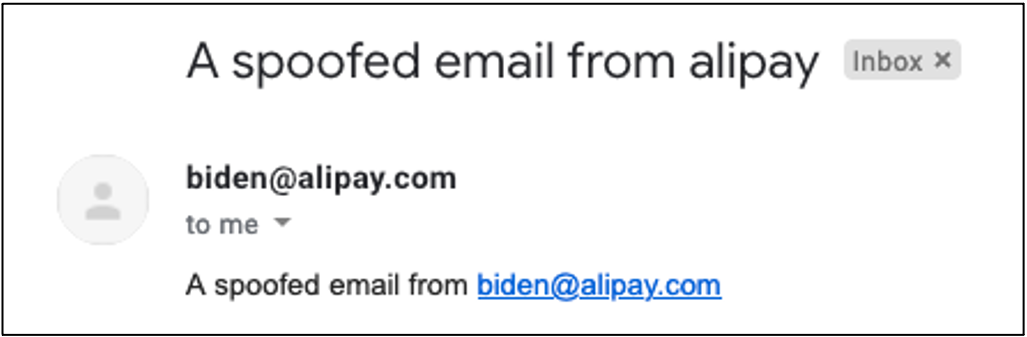
\includegraphics[width=\columnwidth]{graphs/ss_gmail_via_outlook.png}}
  \centering
  \caption{Email spoofing \dns{biden@alipay.com} via Outlook.}
  \label{fig:ss_gmail_via_outlook}
  \end{figure}


\begin{figure}[t]
  \centerline{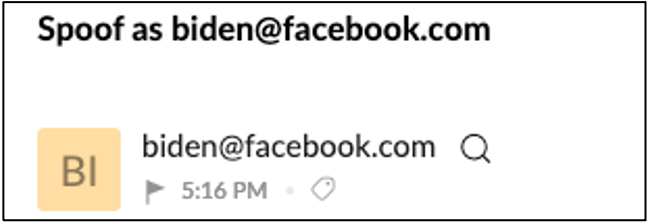
\includegraphics[width=\columnwidth]{graphs/ss_zoho_arc.png}}
  \centering
  \caption{Email spoofing \dns{biden@facebook.com} via Fastmail.}
  \label{fig:ss_zoho_arc}
  \end{figure}

\begin{figure}[t]
\centerline{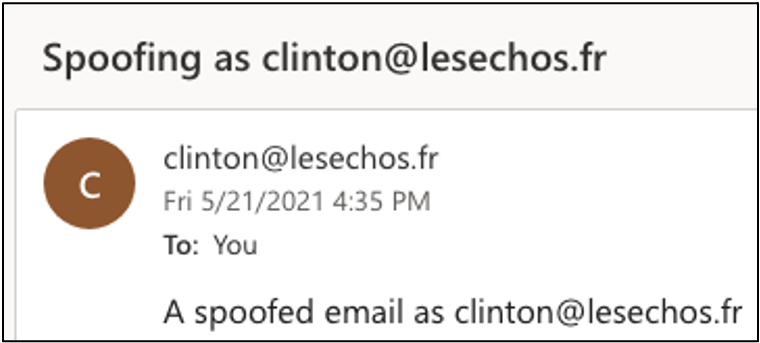
\includegraphics[width=\columnwidth]{graphs/ss_outlook_none.png}}
\centering
\caption{Spoofed email message taking advantage of Outlook's relaxed forwarding validation policy.}
% \geoff{let's see if Stefan notices this screenshot}}
\label{fig:attack_none_ms}
\end{figure}


\section{Additional Details for the Attack in Section~\ref{subsec:attack_zoho_arc}}
\label{sec:appendix_zoho_attack_details}
% \paragraph{Additional Details for the Attack in Section~\ref{subsec:attack_zoho_arc}}
Adversaries can broaden the scope of the attack described in Section~\ref{subsec:attack_zoho_arc} by using a forwarding
account at any email provider that Zoho trusts for ARC purposes,
including Gmail, and routing their spoofed email through multiple forwarding hops.
In particular, an attacker can obtain ARC headers in one forwarding hop via Gmail, and then bypass Gmail's lack of open forwarding by forwarding the email through a second account that does allow open forwarding (\eg, Outlook).
% The attacker can use a Gmail
% account to obtain the necessary ARC headers by including this account as an additional forwarding hop.
% For example, the attacker could create a second
% forwarding account on a platform that has open forwarding (\eg,
% Outlook).
For example, first, the attacker would send their spoofed email message
to their Gmail account, which they configured to forward to their
malicious Outlook account.
During the forwarding process Gmail will
attach a set of ARC headers to the email message.
Next, the spoofed email will arrive at their malicious Outlook account, which then forwards the email to any arbitrary Zoho recipient (because Outlook
supports open forwarding).
This forwarded email message will contain Gmail's attached ARC headers, enabling the attack to successfully pass DMARC validation checks as a result of Zoho's vulnerable ARC implementation.

Using our test accounts, I validated that this multi-hop attack variation
successfully delivers spoofed messages to the inbox of a Zoho recipient
without any warnings.






\section{Additional Details for the Attack in Section~\ref{subsec:attack_none_mailing_list}}
% \paragraph{Additional Details for the Attack in Section~\ref{subsec:attack_none_mailing_list}}
\label{sec:append_mailing_list_details}

% \subsection{Abusing Gaggle.email}

\begin{figure}[t]
\centering
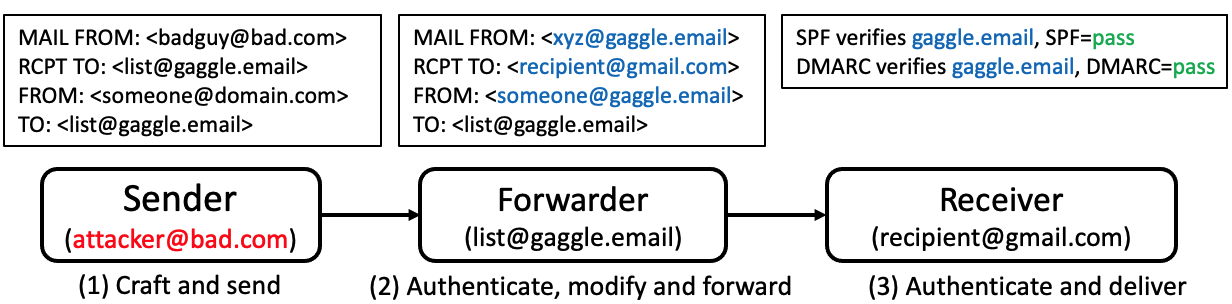
\includegraphics[width=\columnwidth]{graphs/mech_gaggle.png}
\centering
\caption{Attack flow for Gaggle.}
\label{fig:gaggle_email_mech}
\end{figure}

In addition to the attacks described in
Section~\ref{subsec:attack_none_mailing_list}, I found
additional attack variants related to Gaggle.
Figure~\ref{fig:gaggle_email_mech} shows an example of an attack that
abuses Gaggle's use of REM + MOD forwarding
(Section~\ref{sec:measure_forwarding_mechs_and_arc}). This attack works
regardless of the DMARC policy of the spoofed address's domain.  First, an
attacker chooses an address to spoof (\dns{someone@foo.com}) that is
allowed to send to a mailing list on a vulnerable provider
(\dns{list@gaggle.email}), and sends a spoofed email message
purporting to come from that address.  This spoofed email will fail
DMARC validation, but because Gaggle does not enforce DMARC
(Appendix~\ref{subsec:no_dmarc}), it will forward the email to the
mailing list's recipients as normal (Stage 2).  Since Gaggle uses a
REM + MOD forwarding process, it will rewrite the \textsc{MAIL FROM}
header to use the mailing list's domain (\eg, a
new \textsc{MAIL FROM} address of \dns{xyz@gaggle.email}).
%\grant{Similar to earlier, I should be more precise.}
Finally, when the spoofed email message arrives at the recipient's mail server,
it will properly pass SPF validation and DMARC alignment checks:
the rewritten \textsc{MAIL FROM} domain allows the mailing list to send on its behalf, and the domain matches the \textsc{FROM} address's domain (\dns{gaggle.email}).

% \subsection{Other Details}
% Below, I note one additional detail\alex{fix this number} about this attack.

Additionally, I note that mailing list software such as Listserv and
Mailman require a backend MTA.  In our experiments I used Postfix
with DMARC turned on, a configuration which follows good security
practice.  However, in practice many organizations might not use this
configuration because many MTAs (including Postfix) do not enforce
DMARC by default.  In these cases, the attacker can spoof email from any
target domain, regardless of its DMARC policy, much like the attack
against Gaggle.


%\section{Limitations}
%Most of the attacks described in this paper require that the attacker has an account on an email forwarding service and can configure the account to forward email message to the target account. Thus, massively and automatically performing the attacks described in this paper can be challenging. Automating the attacks (e.g., via automated account creation) is out of scope for this work.


\end{document}
